\documentclass[12pt]{article}
\usepackage[utf8x]{inputenc}
\usepackage{url}
\usepackage{lipsum}
\usepackage{graphicx}
\usepackage{color}
\usepackage{amsmath}
\usepackage{amssymb}
\graphicspath{{./figs/}}
\DeclareGraphicsExtensions{.pdf,.jpeg,.jpg,.png}
\usepackage{hyperref}
\usepackage{cleveref}
\Crefname{figure}{Fig.}{Figs.}
\usepackage{todonotes}
\setlength{\marginparwidth}{3.5cm}
\usepackage[acronym]{glossaries}
\usepackage{subfig}
\usepackage{array}
\usepackage{rotating}
\usepackage{siunitx}
\usepackage{tabu}
\usepackage{hhline}
\usepackage{boldline} 
\captionsetup[subfigure]{subrefformat=simple,labelformat=simple}
    \renewcommand\thesubfigure{(\alph{subfigure})}
\usepackage{makecell}
\usepackage{longtable}
\newacronym{aod}{AoD}{angle-of-departure}
\newacronym{aoa}{AoA}{angle-of-arrival}
\newcommand{\areaofinterestfigwidth}{1.0\textwidth}
\newcommand{\vspaceintitle}{\vspace{5mm}}

\title{
    \vspace{-30mm}
    \begin{figure}[h]
        \centering
        
\includegraphics[width=3in]{ece-horizontal-black-and-gold-rgb}
    \end{figure}
    \vspaceintitle
    \large Site-Specific Millimeter-Wave Propagation Modeling \\
        for Wide Area Wireless Networks \\
    \vspaceintitle
    \huge NSF PAWR POWDER-RENEW Testbed Measurement Plan\\
    \vspaceintitle
    \Large DRAFT v3.0}
\author{Bharath Keshavamurthy and Yaguang Zhang, Purdue University\\
Dr. Chris Anderson, United State Naval Academy}

\begin{document}
\maketitle
\tableofcontents
\newpage

\section{Objective \& Background}
    The objective of this measurement campaign is to obtain a reasonably large dataset of site-specific signal propagation characteristics for experimenting Artificial Intelligence (A.I.) algorithms in mmWave radio ecosystems. Measurements will be performed on the NSF PAWR POWDER-RENEW testbed at the University of Utah in Salt Lake City, UT, to emulate typical $5$G (and beyond) deployments in urban and suburban environments. The Tx will be temporarily installed at designated points on the roof of several buildings at the University of Utah (e.g., University of Utah Hospital Building, Behavioral Sciences Building, etc). The Rx, on the other hand, would be mounted on top of a van, and driven around campus along pre-determined routes (e.g., Blue Detour, Suburban, etc) to collect these geographically correlated measurements -- intended to be used for transmission loss evaluations in direct-link large-scale propagation modeling and for beam-steering/multipath evaluations under different \gls{aod}/\gls{aoa} values. \\

    \noindent Electromagnetic signals in the mmWave bands are expected to experience more attenuation over distance and be extremely sensitive to obstacles in the environment. To take full advantage of the vast mmWave bandwidth to be available in next-generation radio access technologies, service providers will need channel information based on Tx and Rx locations in both planning and operating these networks: a comprehensive channel measurement dataset with detailed geographic information is the key to fostering these site-specific mmWave channel models. In this measurement campaign, we would like to create such a dataset for urban and suburban environments at $28$GHz. Two types of measurement results are planned to be extracted: 
    \begin{itemize}
        \item Transmission loss assessments of the direct link between a fixed Tx and a mobile Rx covering a reasonably large geographic area (${\approx}1$ sq. km) for large-scale site-specific propagation modeling, and
        \item Transmission loss assessments at pre-determined Rx locations with a pre-assigned combination of different \gls{aod}/\gls{aoa} values for multipath evaluation.
    \end{itemize}

\section{Methodology}
    \subsection{Introduction}
        \begin{figure}
            \centering
            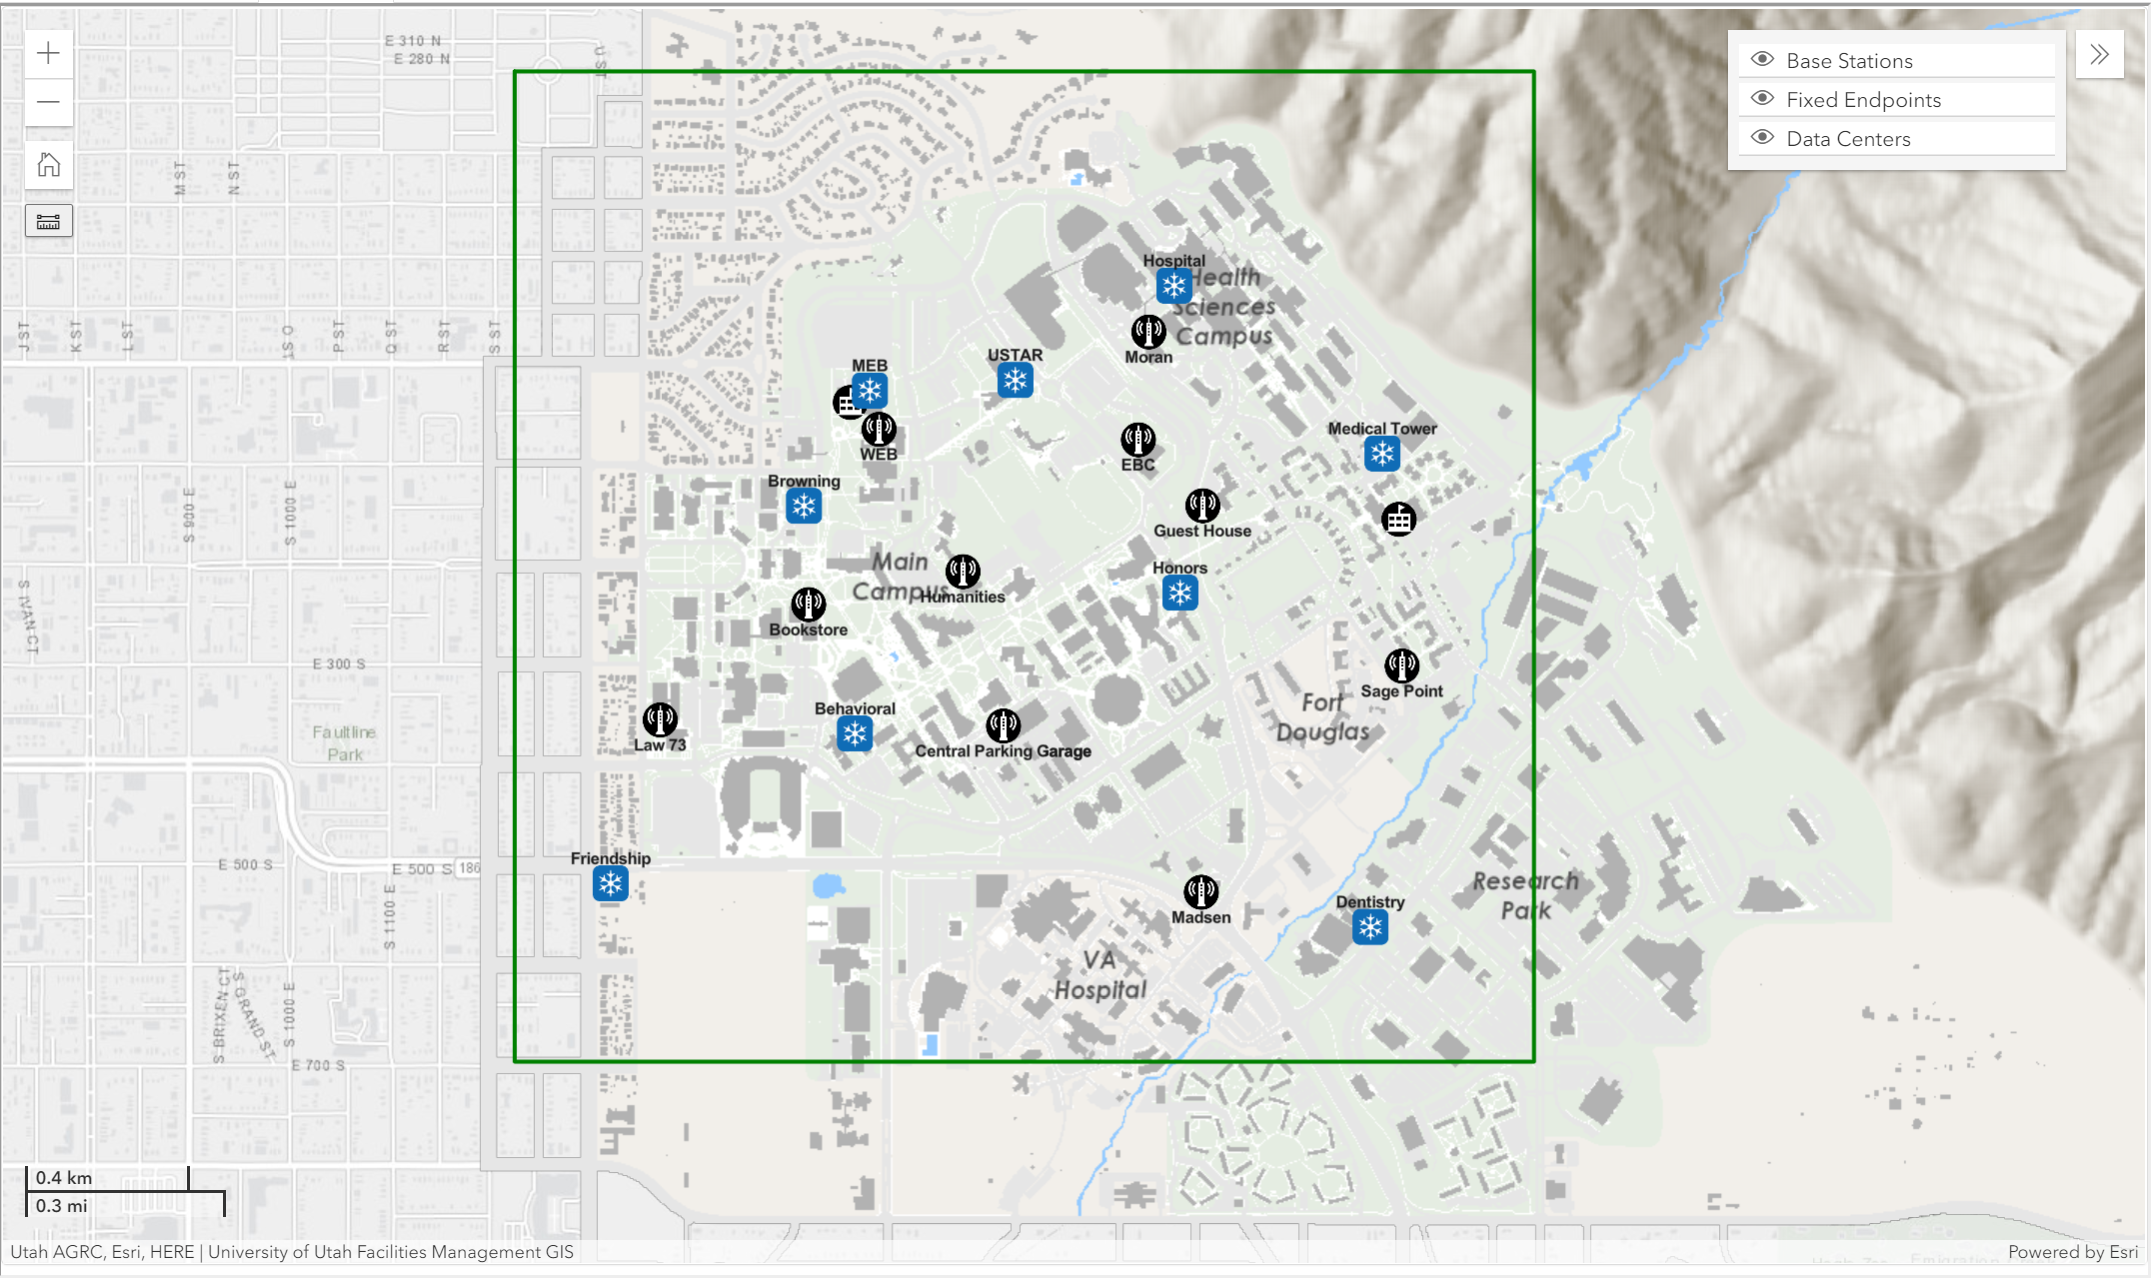
\includegraphics[width=\areaofinterestfigwidth]{figs/POWDER_Map.png}
            \caption{The NSF PAWR POWDER-RENEW testbed at the University of Utah: our measurement arena}
            \label{fig:map}
        \end{figure}
        The measurement campaign will be conducted using a pair of autonomous antenna tracking platforms -- one at the Tx and another at the Rx -- developed under Project Odin at Purdue University, in collaboration with Dr. Chris Anderson of the United States Naval Academy (USNA). Details about our sounder design at $28$GHz are provided in Sec. \ref{S3.5}, and details about our autonomous antenna tracking platforms are outlined in Sec. \ref{S3.6}. Finally, introducing our playground, \Cref{fig:map} depicts our arena for this measurement campaign -- constituting both urban and suburban environments in and around the University of Utah.
        \clearpage
        
    \subsection{Potential Tx Mount-Point Candidates}\label{S3.2}
       \begin{itemize}
            \begin{figure}
                \centering
                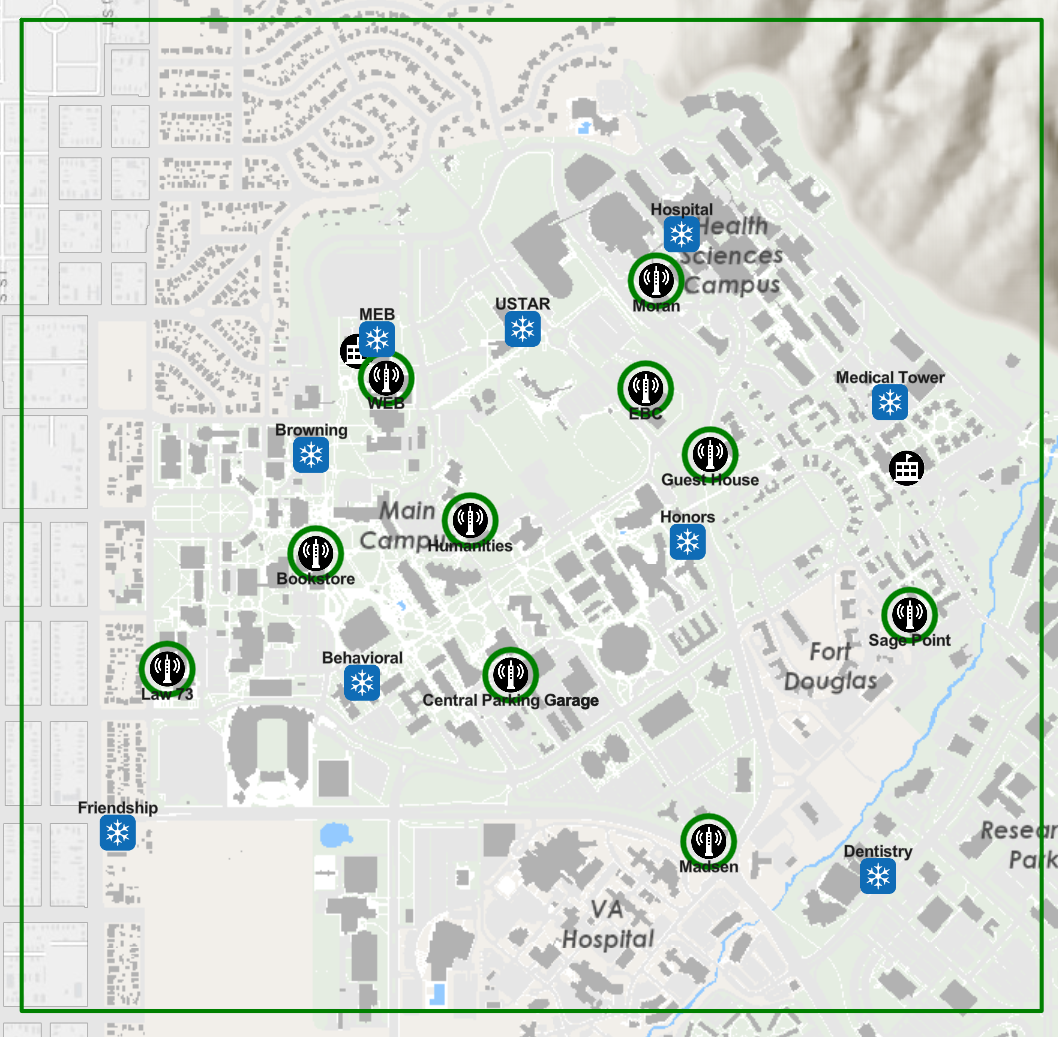
\includegraphics[width=\areaofinterestfigwidth]{figs/Location_Scout_Fixed_Endpoints.png}
                \caption{Potential Tx mount-point candidates: The fixed end-points (with their associated Intel NUC small form-factor compute nodes) available for provisioning on the University of Utah's POWDER testbed}
                \label{fig:fixed}
           \end{figure}
            \item \Cref{fig:fixed} illustrates a set of potential Tx mount-points at the University of Utah -- designated as ``fixed end-points" on the POWDER testbed -- with their corresponding USRP B$210$ radios and Intel NUC small form-factor compute nodes; and
            
            \begin{figure}
                \centering
                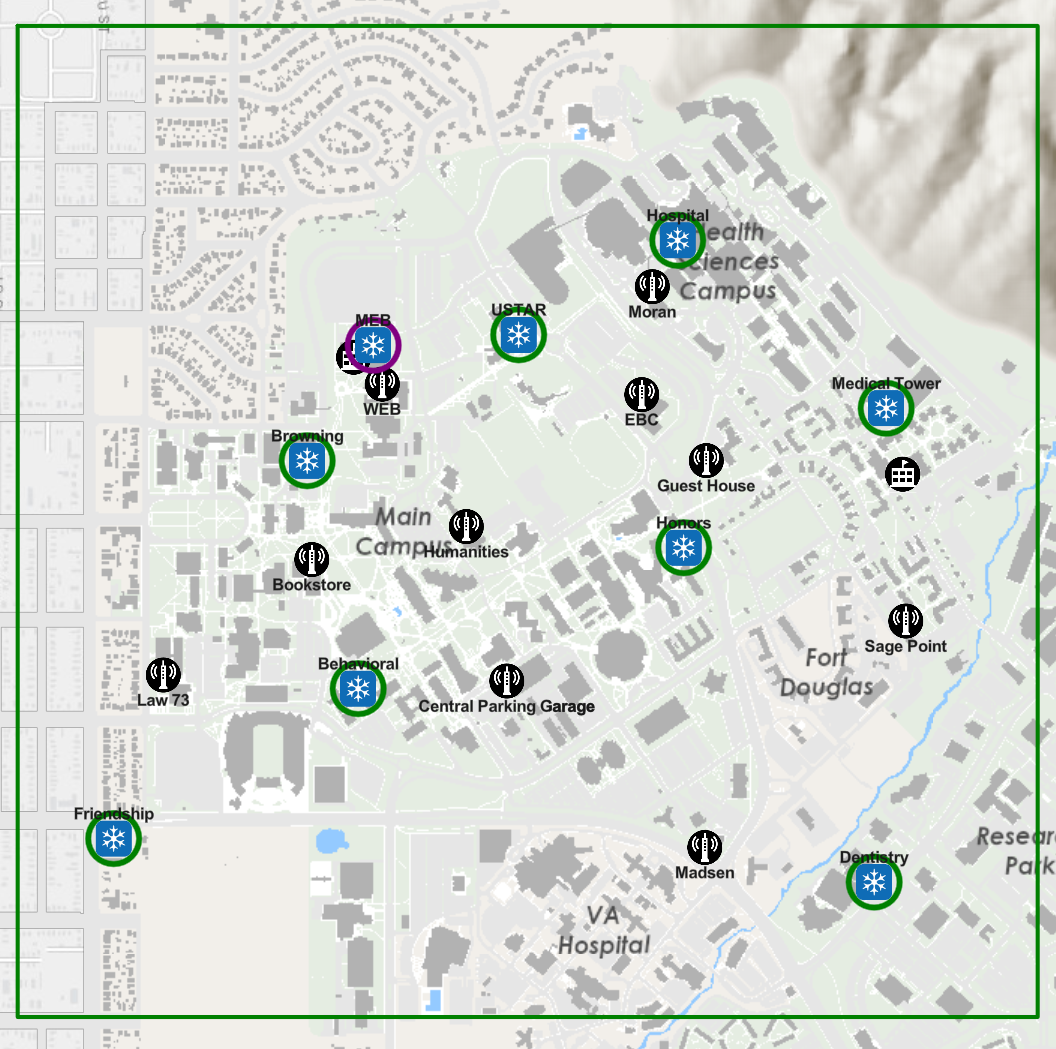
\includegraphics[width=\areaofinterestfigwidth]{figs/Location_Scout_Rooftop_Candidates.png}
                \caption{Potential Tx mount-point candidates: The roof-top base-stations (with their associated Dell PowerEdge compute nodes) available for provisioning on the University of Utah's POWDER testbed}
                \label{fig:roof}
           \end{figure}
            \item \Cref{fig:roof} illustrates another set of potential Tx mount-points -- designated as ``roof-top base-stations" on the POWDER testbed -- with their corresponding USRP X$310$ radios and more powerful Dell PowerEdge R740/R840 compute nodes.
       \end{itemize}
            
    \subsection{Potential Mobile Rx Routes}\label{S3.3}
    Although some of the following routes match the routes of the ``mobile nodes" (shuttles) available on the POWDER testbed, we do not intend to use these shuttles for our measurement campaign; instead, we would provision a van on our own and mount our Rx setup on top of it.
        \begin{itemize}
            \begin{figure}
                \centering
                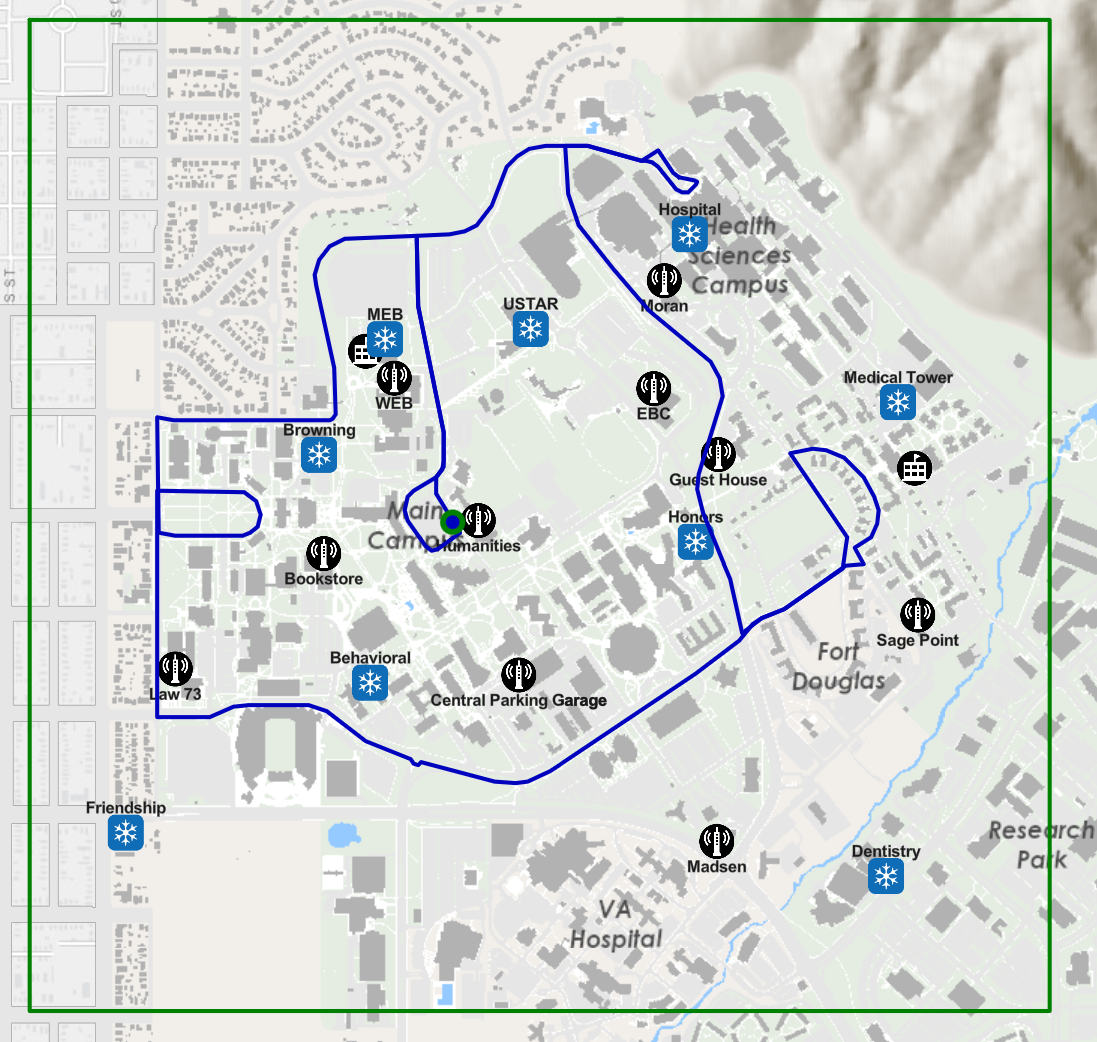
\includegraphics[width=\areaofinterestfigwidth]{figs/Blue_Detour_Route_5.png}
                \caption{The ``Blue Detour" route around the University of Utah campus -- to be traversed by the Rx}
                \label{fig:Rx_1}
            \end{figure}
            \begin{figure}
                \centering
                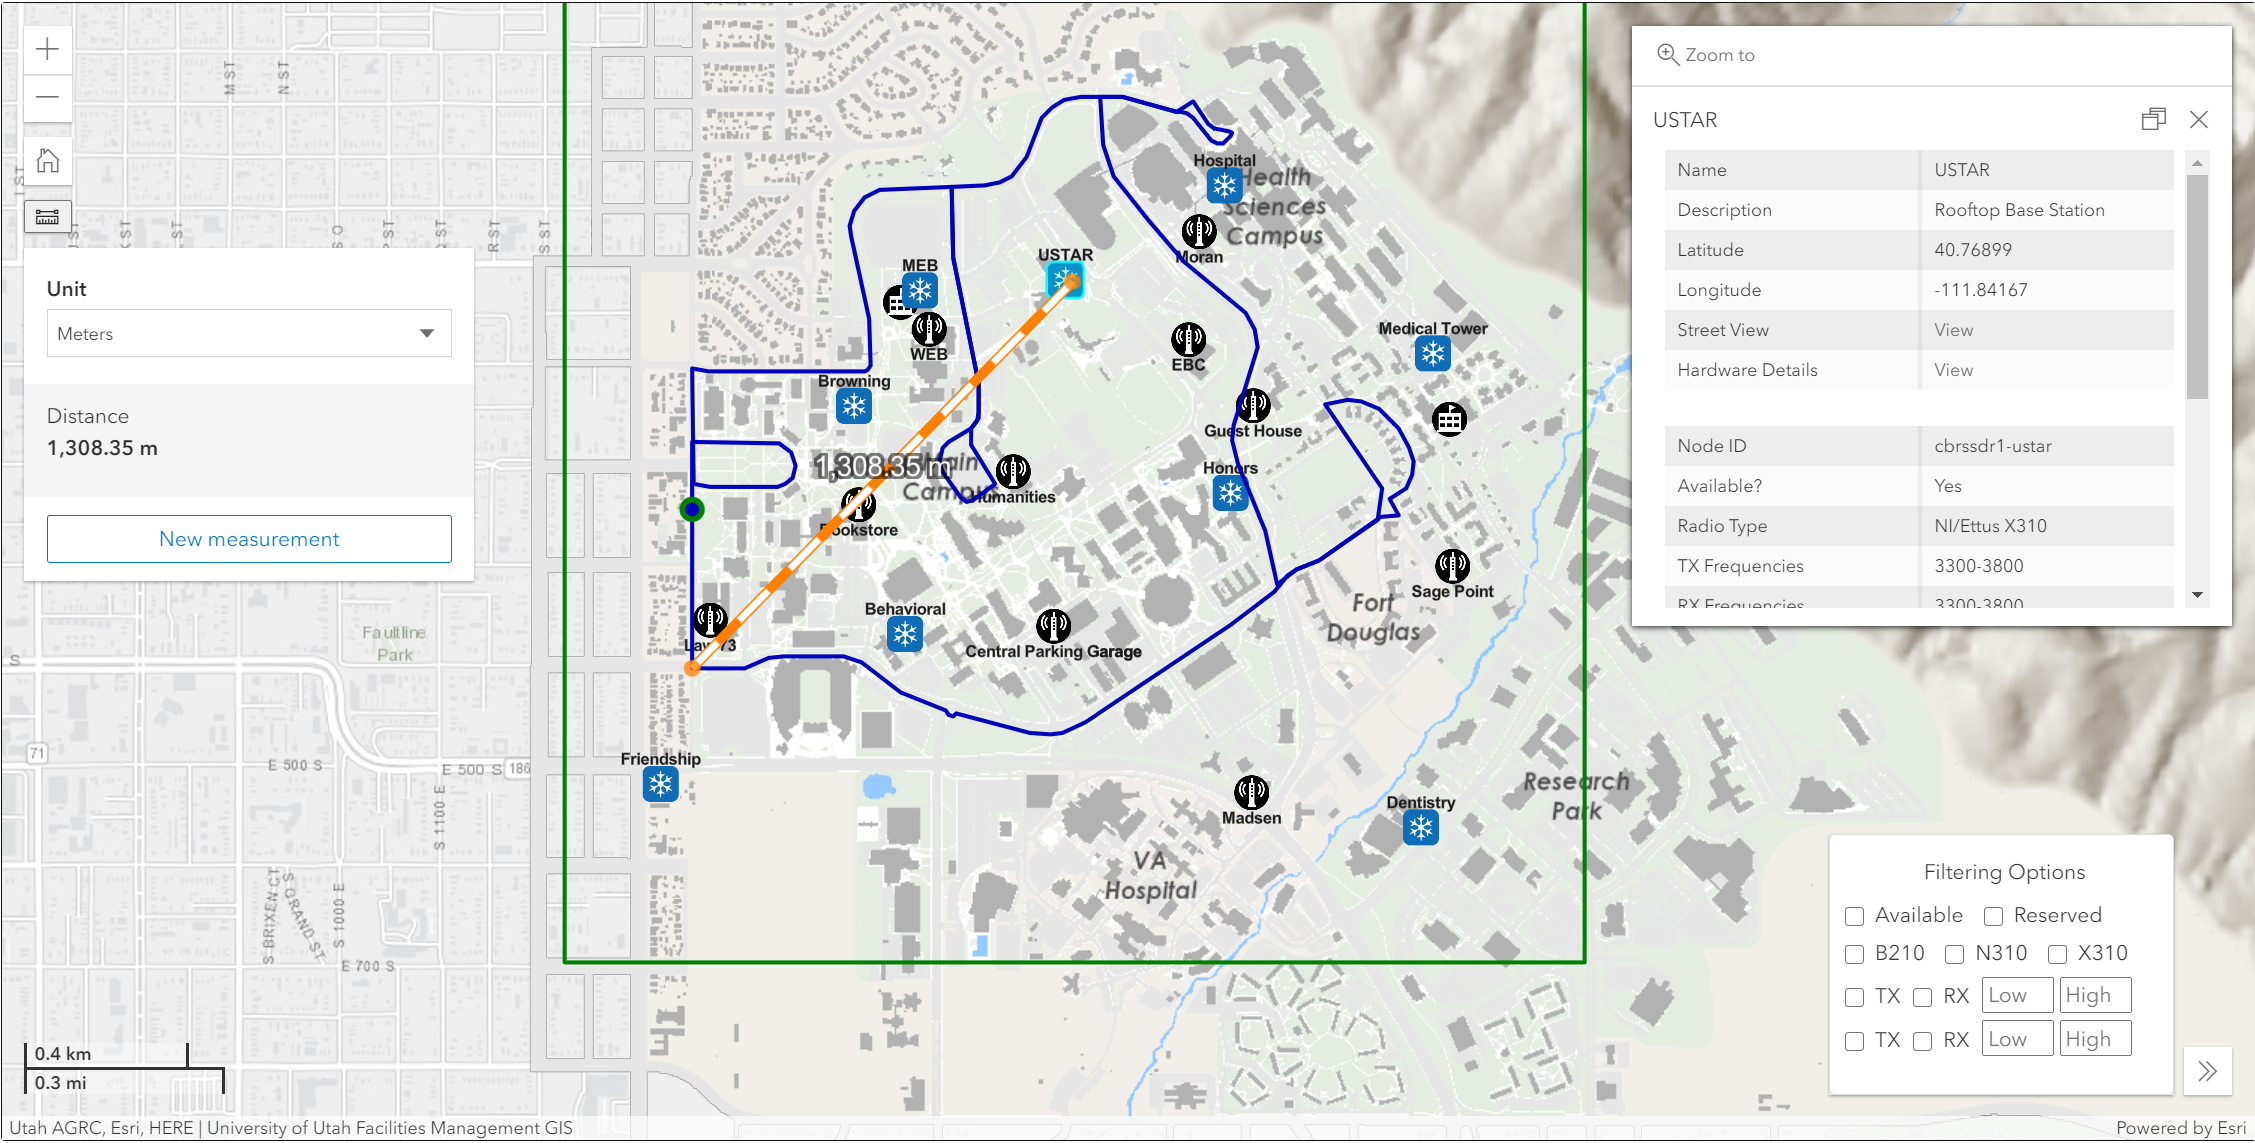
\includegraphics[width=\areaofinterestfigwidth]{figs/Blue_Detour_Route_5_USTAR_Tx.png}
                \caption{The location of the Tx (fixed) while the Rx moves along the ``Blue Detour" route}
                \label{fig:Tx_1}
            \end{figure}
            \begin{figure}
                \centering
                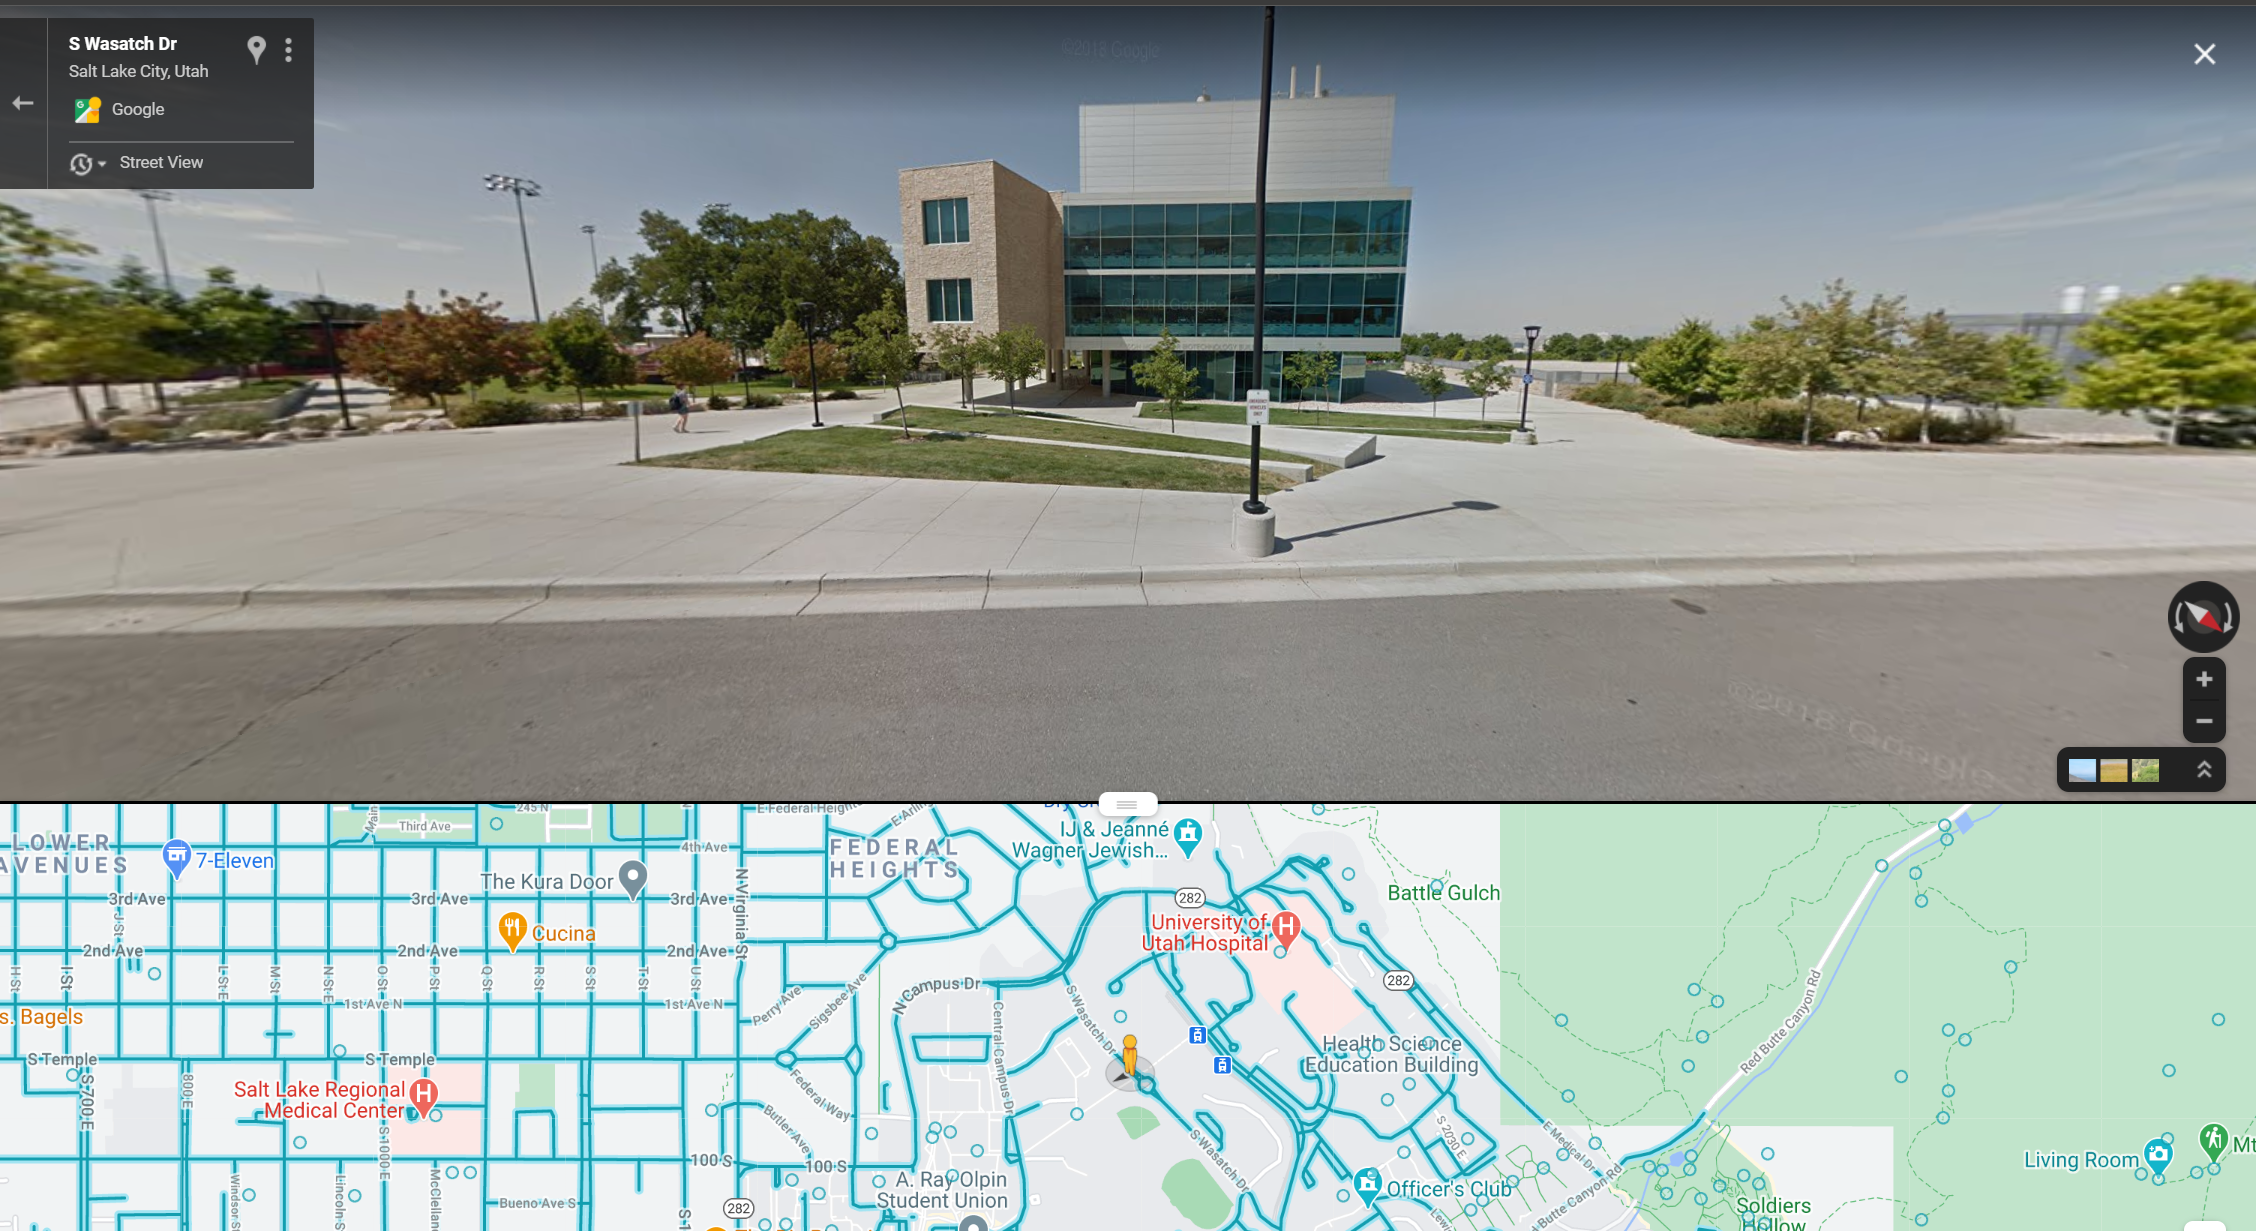
\includegraphics[width=\areaofinterestfigwidth]{figs/USTAR_Tx.png}
                \caption{A street view of the USTAR Building Tx mount point for the ``Blue Detour" Rx route}
                \label{fig:Tx_1_details}
            \end{figure}
            \begin{figure}
                \centering
                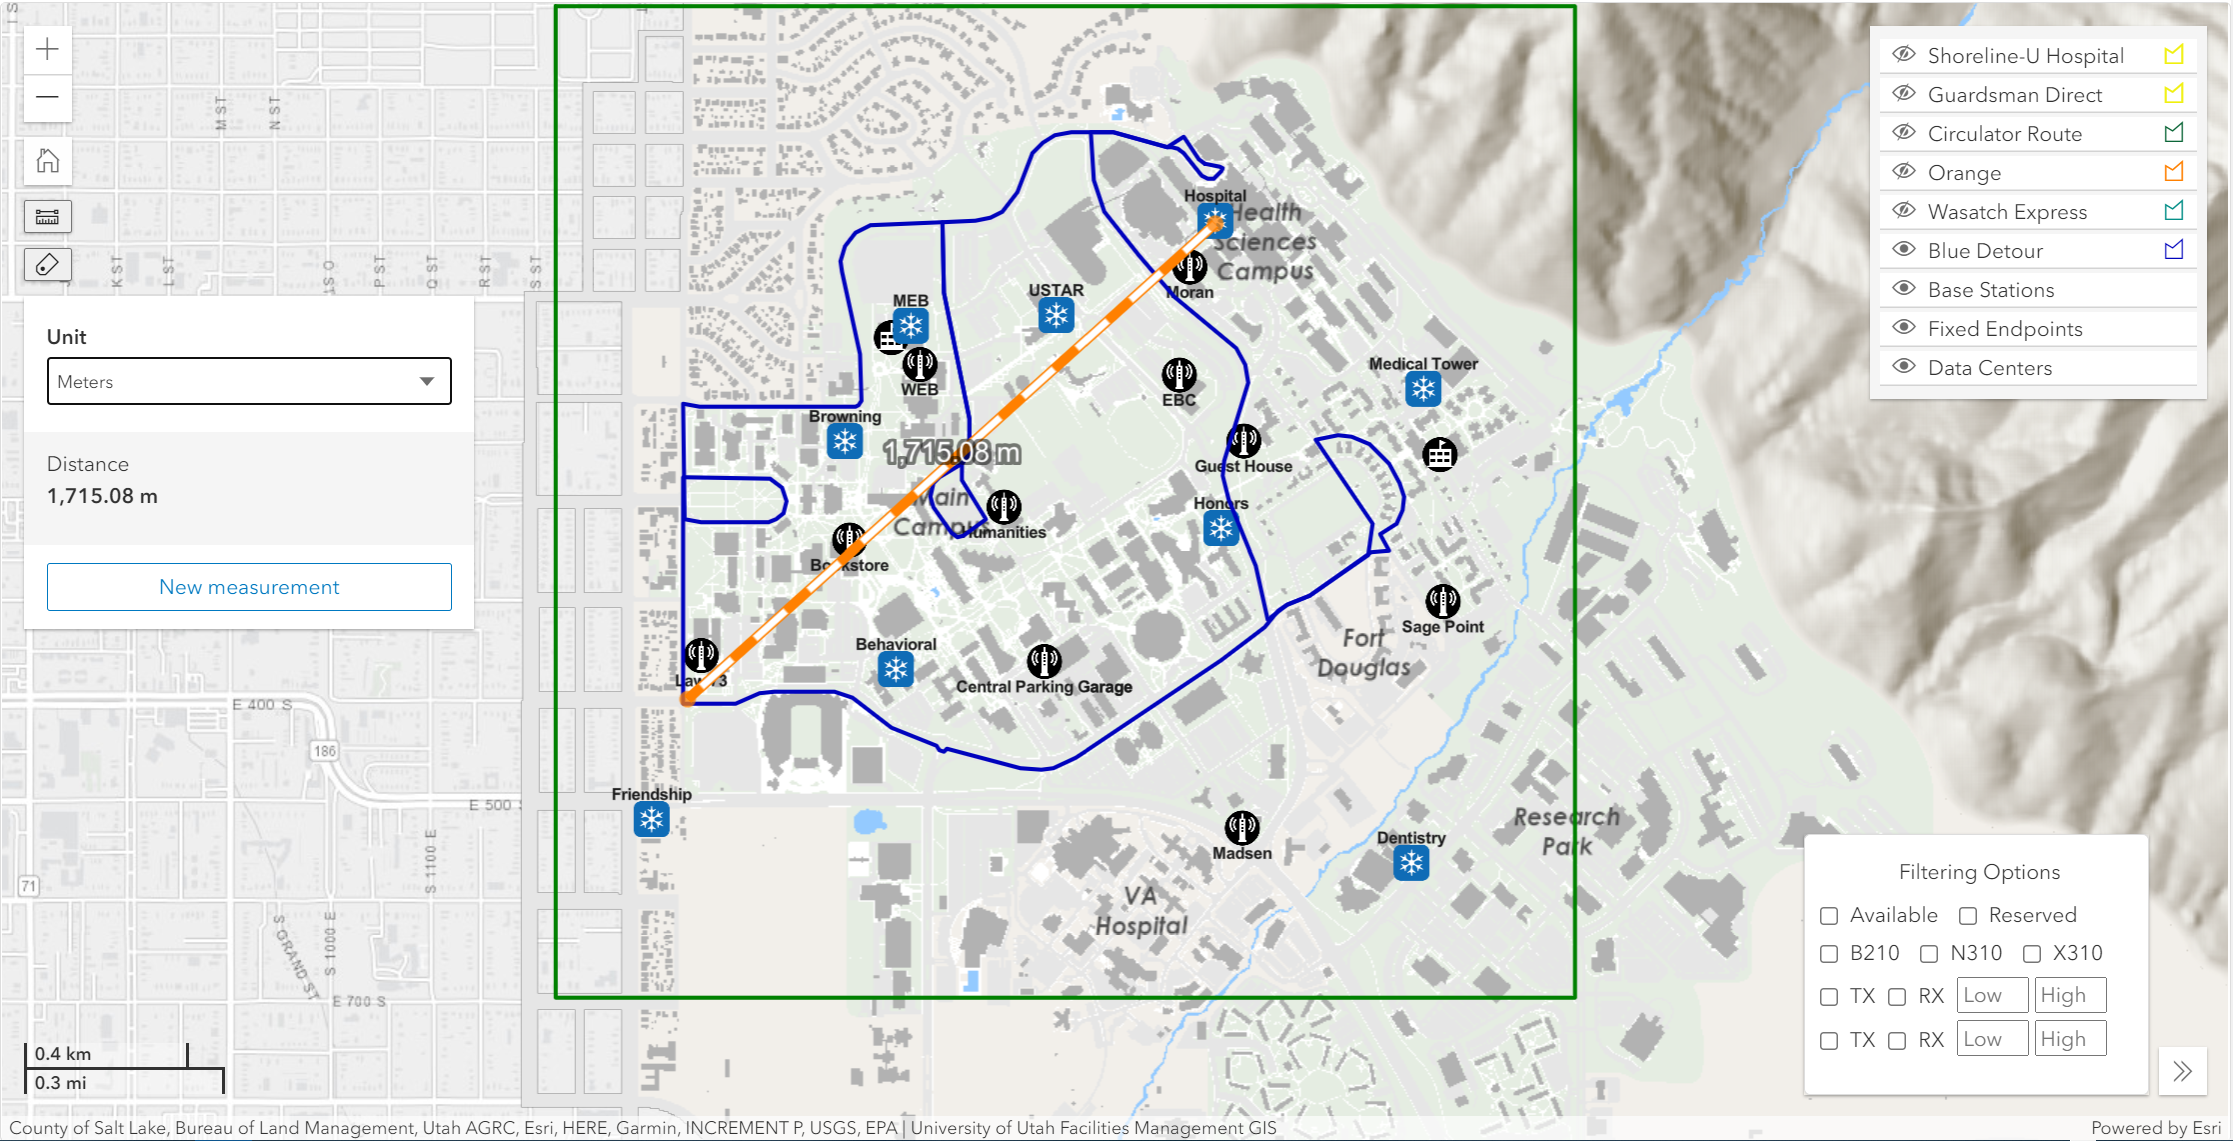
\includegraphics[width=\areaofinterestfigwidth]{figs/Blue_Detour_Route_5_Hospital_Tx.png}
                \caption{The location of the Tx (fixed) while the Rx moves along the ``Blue Detour" route}
                \label{fig:Tx_1a}
            \end{figure}
            \begin{figure}
                \centering
                \includegraphics[width=\areaofinterestfigwidth]{figs/Hospital_Tx.png}
                \caption{A street view of the University of Utah Hospital Building Tx mount point for the ``Blue Detour" Rx route}
                \label{fig:Tx_1a_details}
            \end{figure}
            \item \underline{Blue Detour}: Rx along the route depicted in \Cref{fig:Rx_1} -- with the Tx affixed at the mount-point depicted in \Cref{fig:Tx_1} and \Cref{fig:Tx_1_details} -- for site-specific mmWave propagation modeling in urban environments;
            
            \begin{figure}
                \centering
                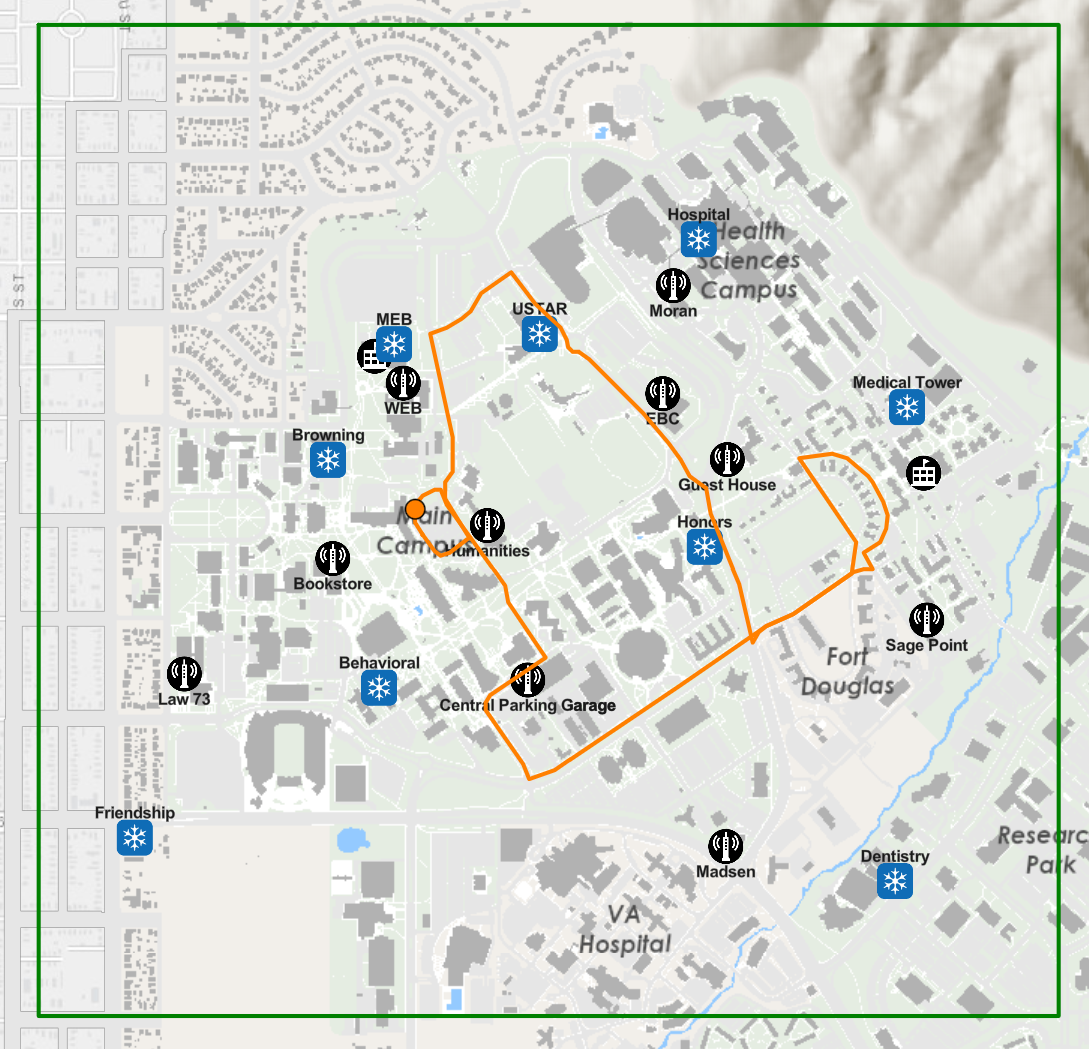
\includegraphics[width=\areaofinterestfigwidth]{figs/Orange_Route_3.png}
                \caption{The ``Orange" route around the University of Utah campus -- to be traversed by the Rx}
                \label{fig:Rx_2}
            \end{figure}
            \begin{figure}
                \centering
                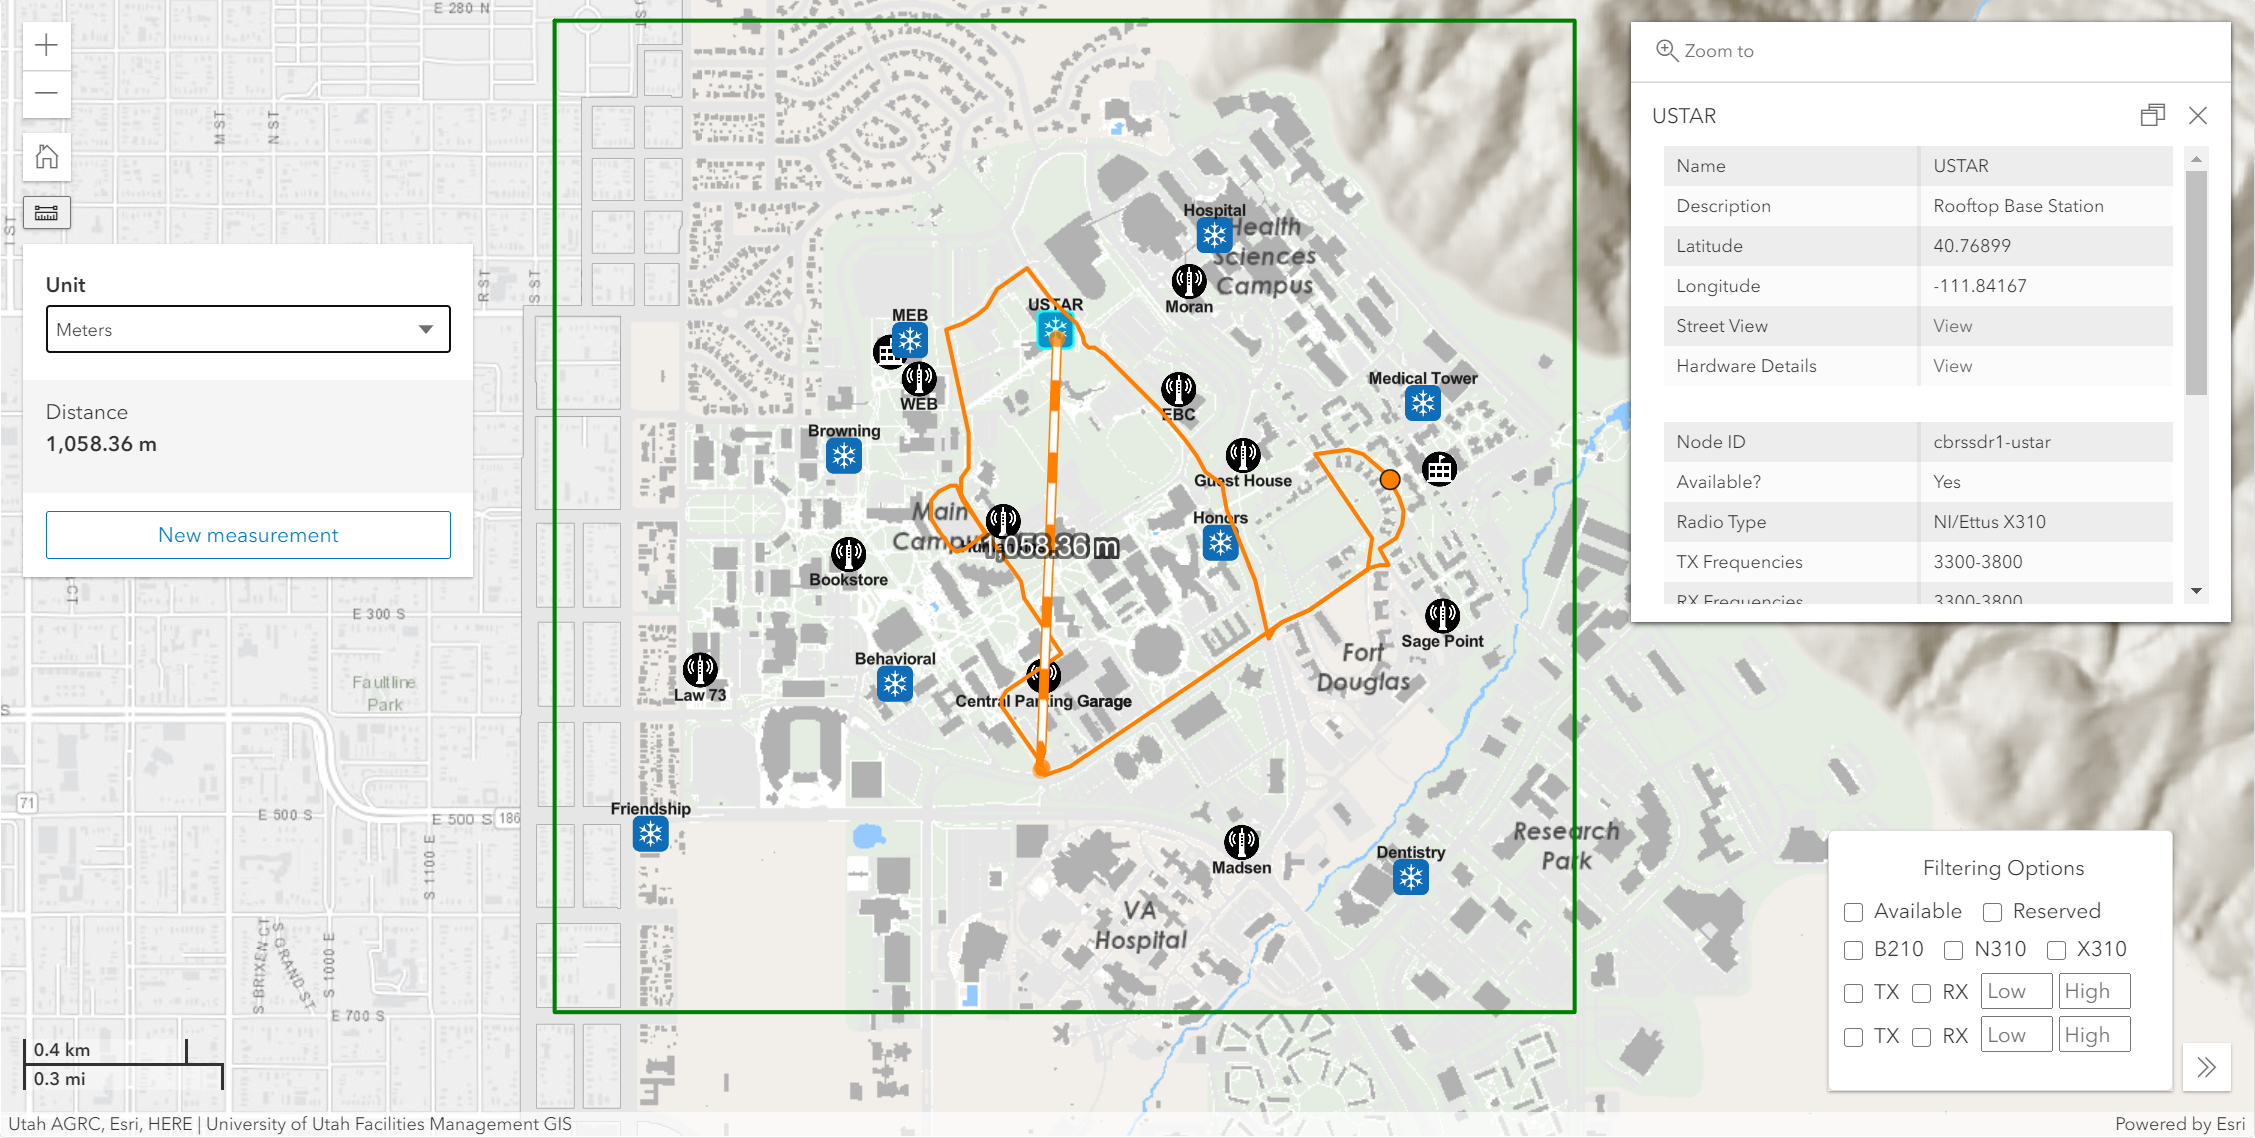
\includegraphics[width=\areaofinterestfigwidth]{figs/Orange_Route_3_with_USTAR_Tx.png}
                \caption{The location of the Tx (fixed) while the Rx moves along the ``Orange" route}
                \label{fig:Tx_2}
            \end{figure}
            \begin{figure}
                \centering
                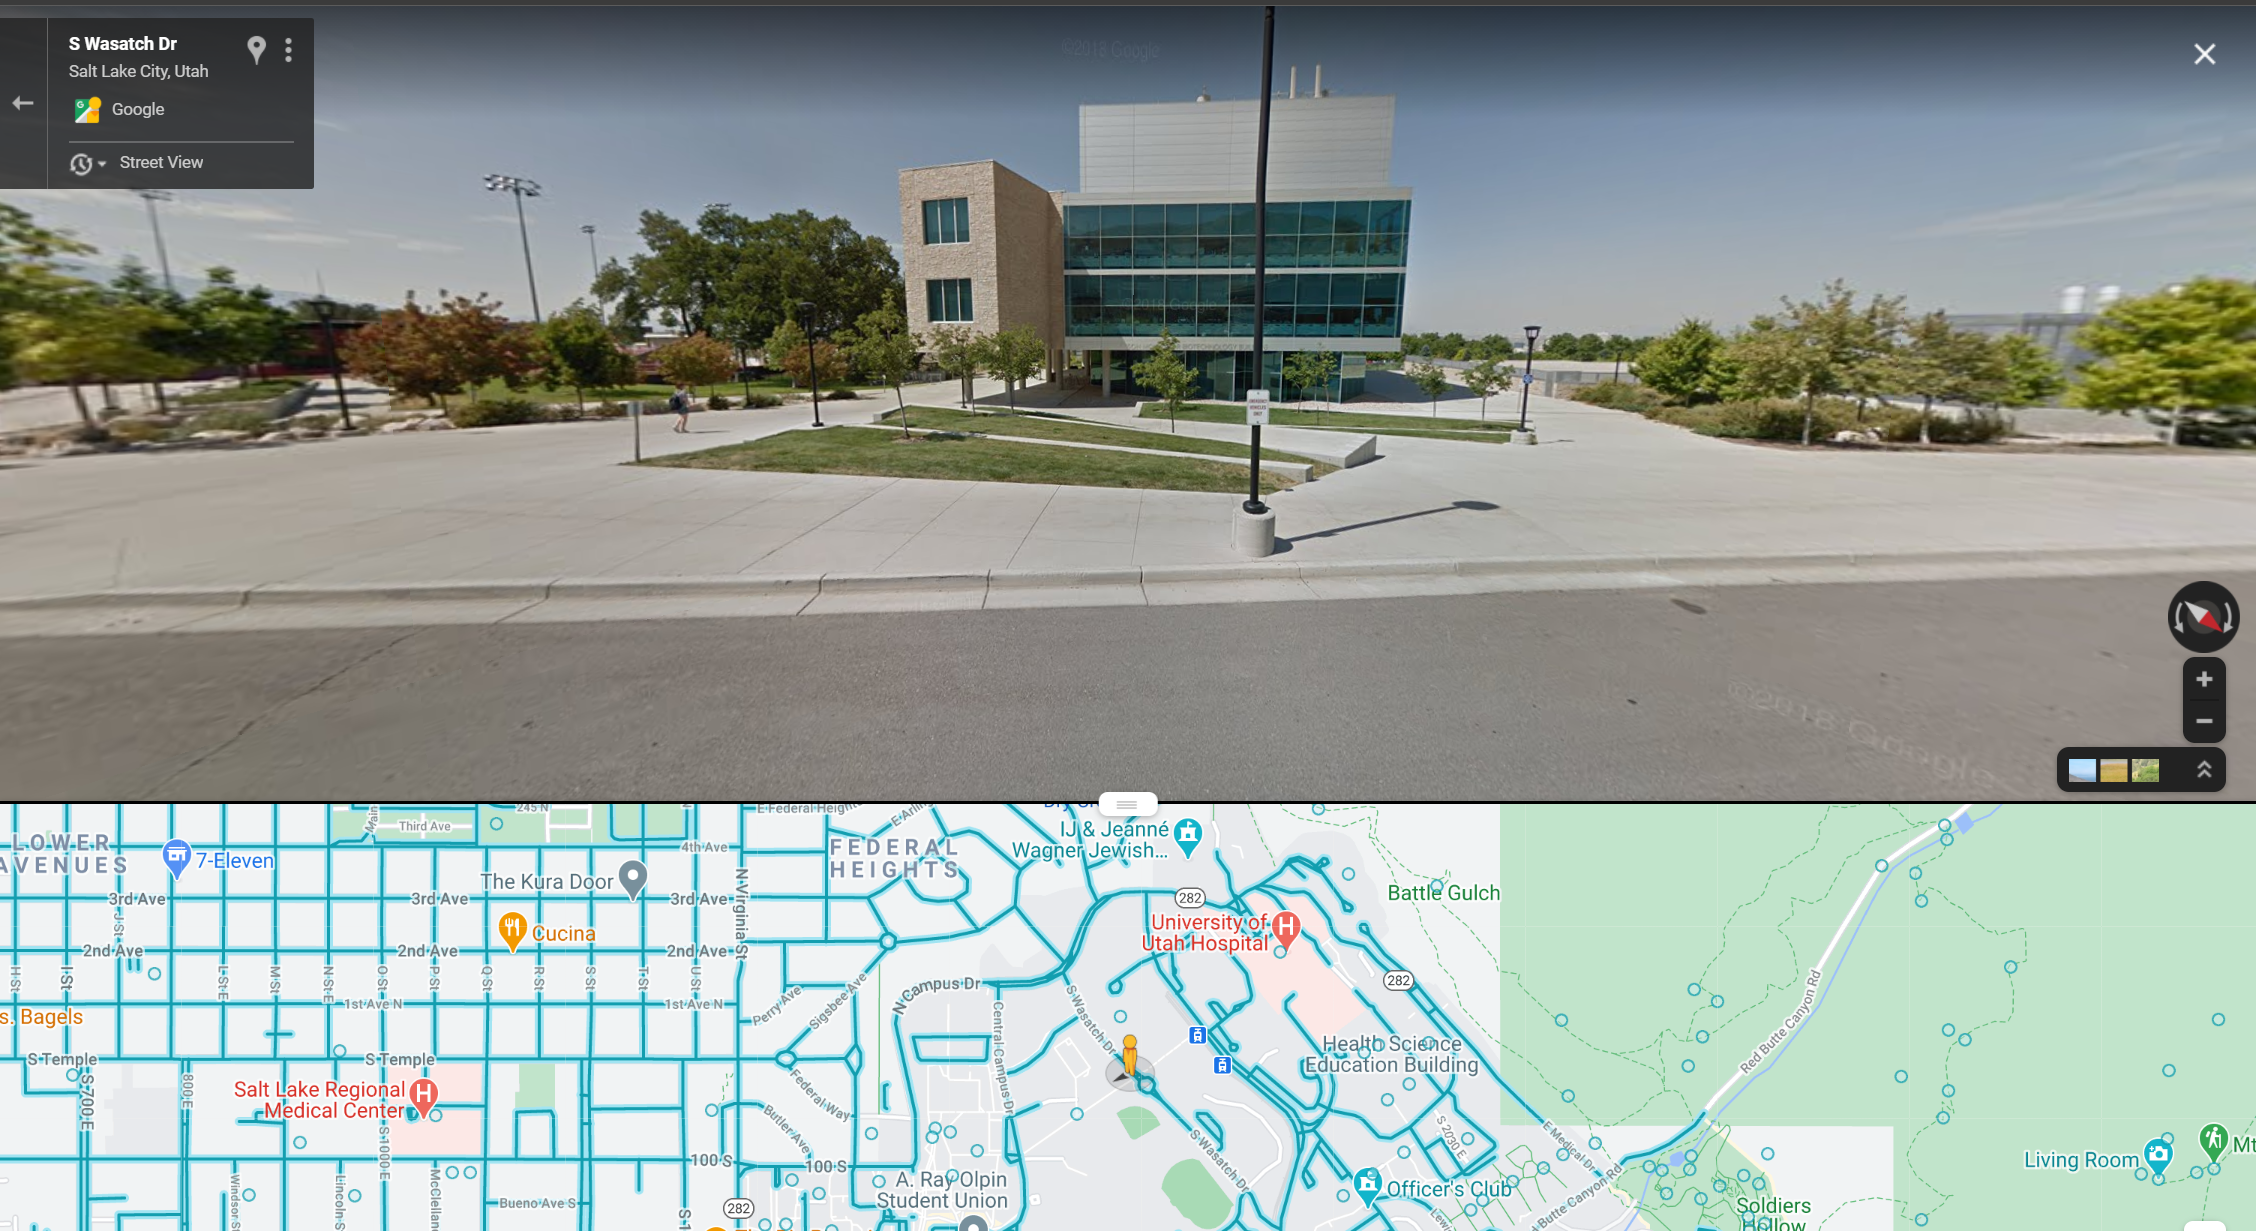
\includegraphics[width=\areaofinterestfigwidth]{figs/USTAR_Tx.png}
                \caption{A street view of the USTAR Building Tx mount point for the ``Orange" Rx route}
                \label{fig:Tx_2_details}
            \end{figure}
            \item \underline{Orange}: Rx along the route depicted in \Cref{fig:Rx_2} -- with the Tx affixed at the mount-point depicted in \Cref{fig:Tx_2} and \Cref{fig:Tx_2_details} -- for site-specific mmWave propagation modeling in urban environments;
            
            \begin{figure}
                \centering
                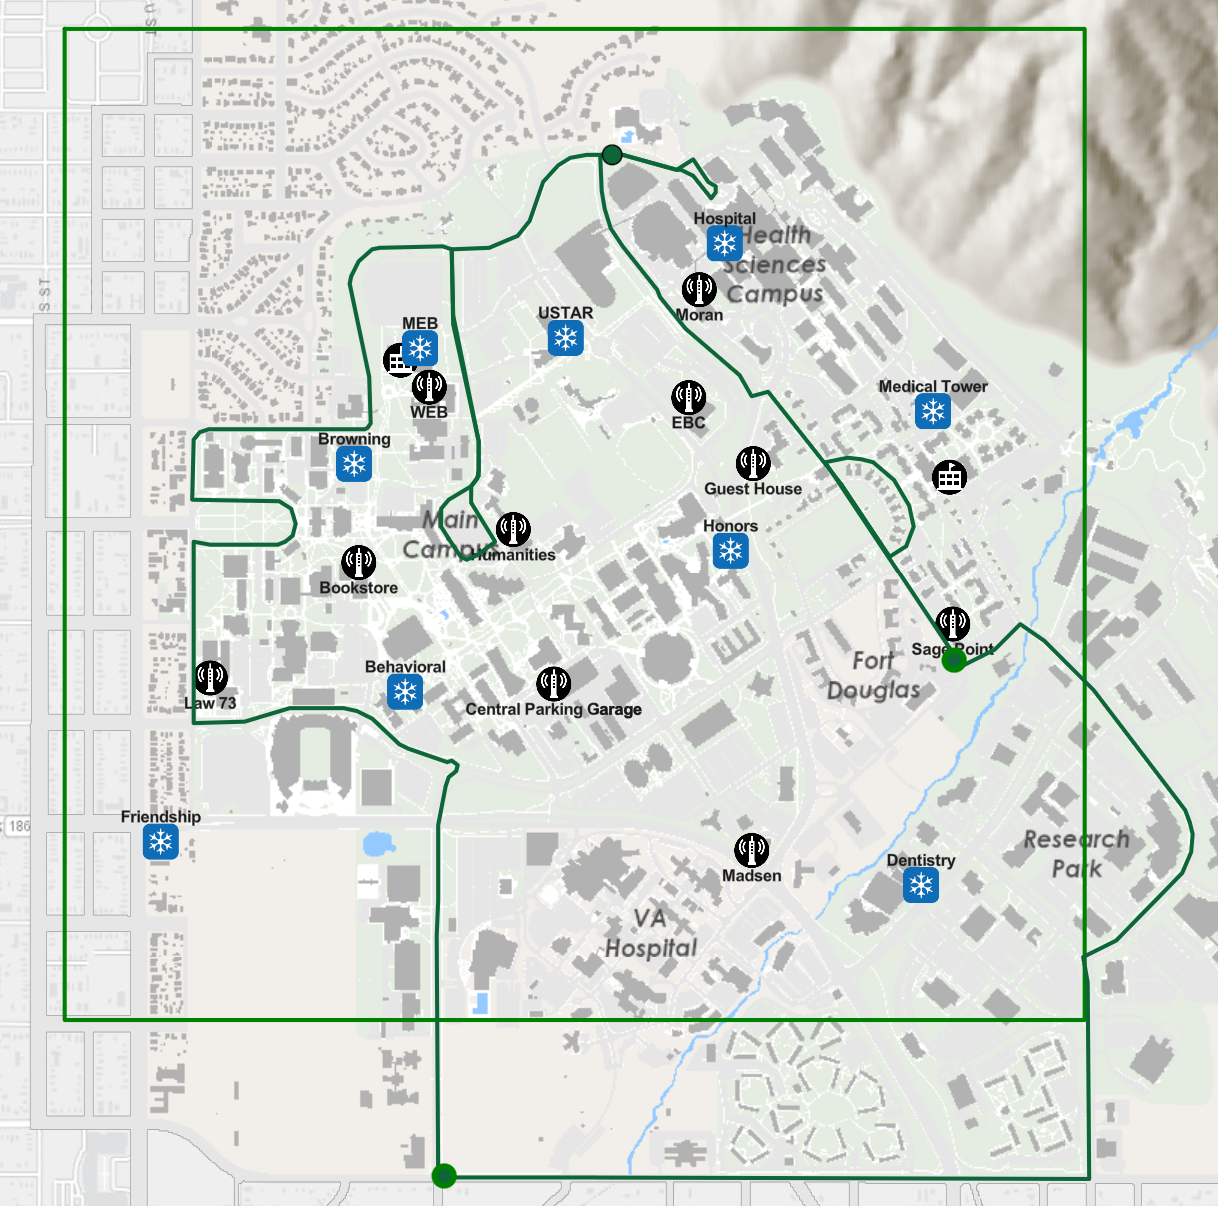
\includegraphics[width=\areaofinterestfigwidth]{figs/Circulator_Route_2.png}
                \caption{The ``Circulator" route around the University of Utah campus -- to be traversed by the Rx}
                \label{fig:Rx_3}
            \end{figure}
            \begin{figure}
                \centering
                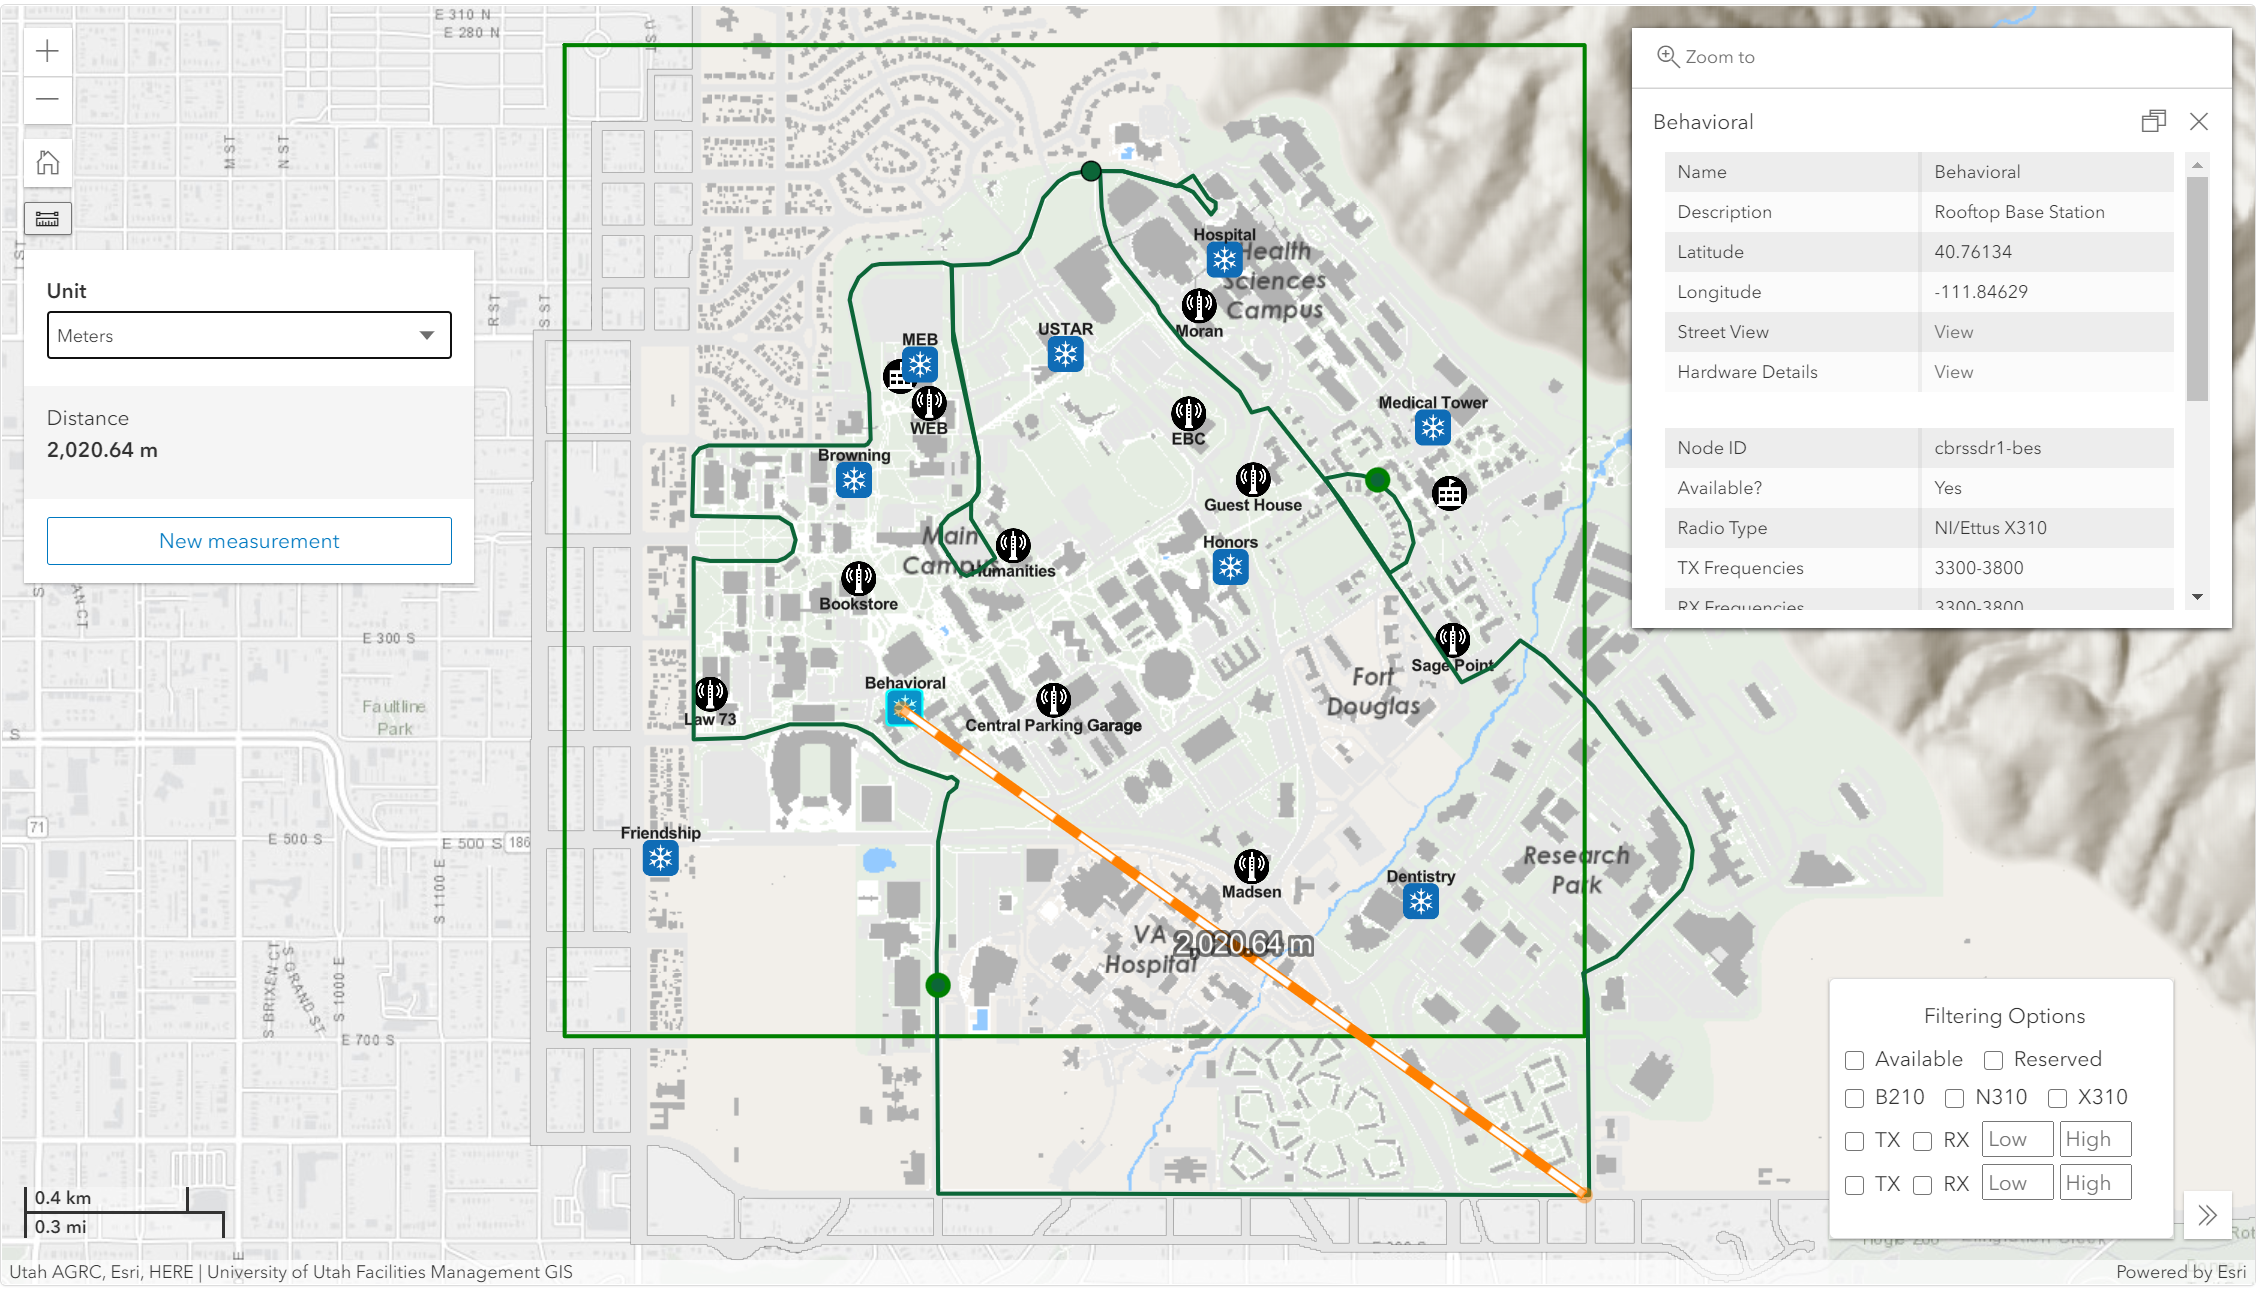
\includegraphics[width=\areaofinterestfigwidth]{figs/Circulator_Route_2_Behavioral_Tx.png}
                \caption{The location of the Tx (fixed) while the Rx moves along the ``Circulator" route}
                \label{fig:Tx_3}
            \end{figure}
            \begin{figure}
                \centering
                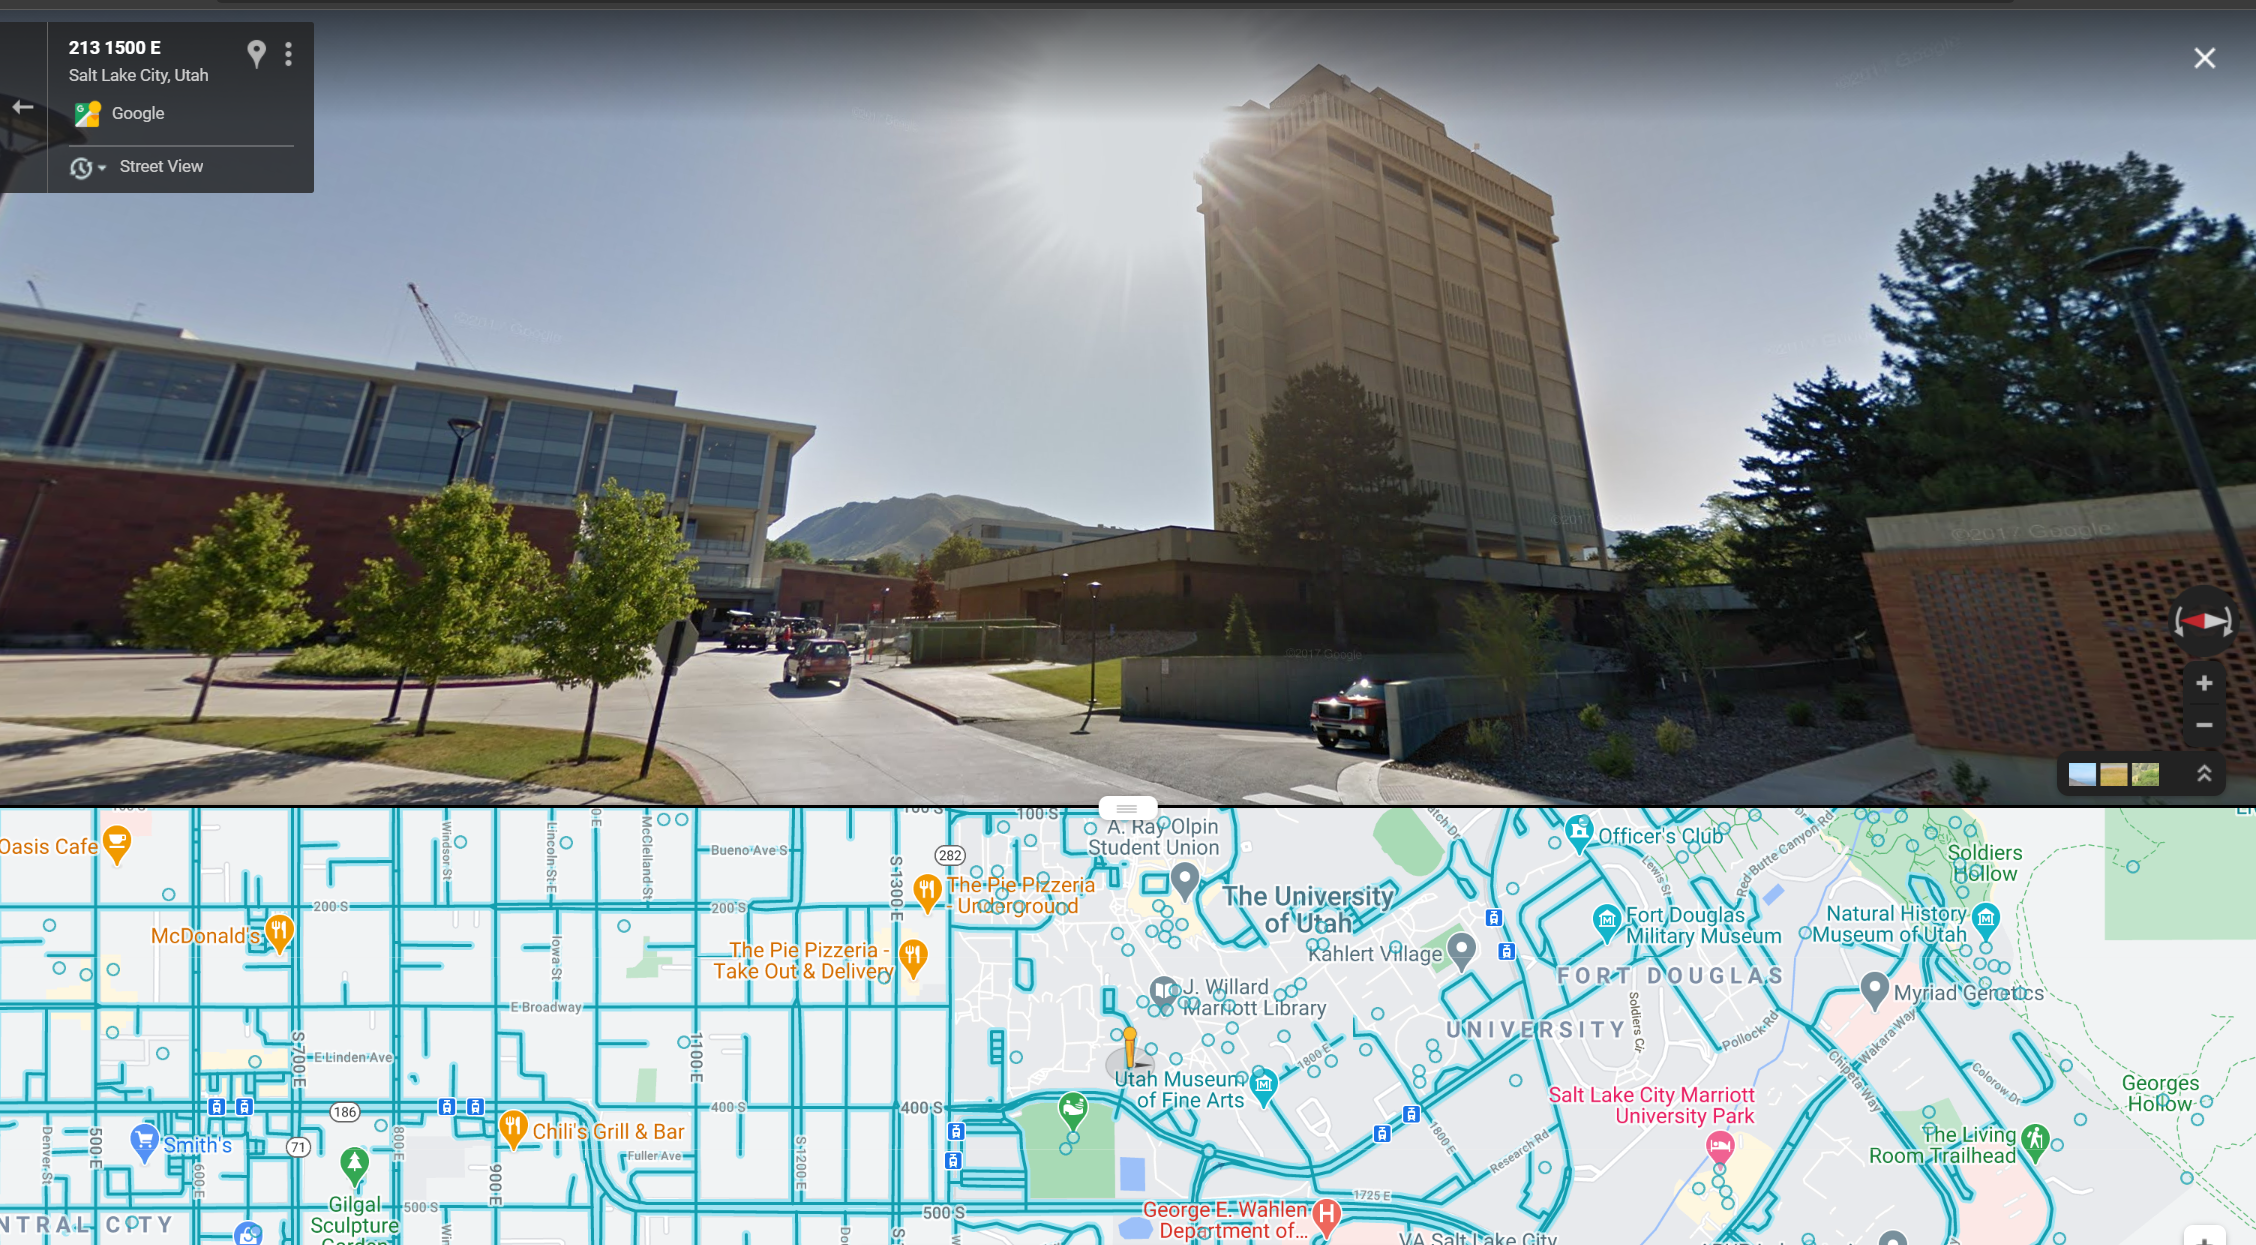
\includegraphics[width=\areaofinterestfigwidth]{figs/Behavioral_Tx.png}
                \caption{A street view of the Behavioral Sciences Building Tx mount point for the ``Circulator" Rx route}
                \label{fig:Tx_3_details}
            \end{figure}
            \item \underline{Circulator}: Rx along the route depicted in \Cref{fig:Rx_3} -- with the Tx affixed at the mount-point depicted in \Cref{fig:Tx_3} and \Cref{fig:Tx_3_details} -- for site-specific mmWave propagation modeling in urban environments;
            
            \begin{figure}
                \centering
                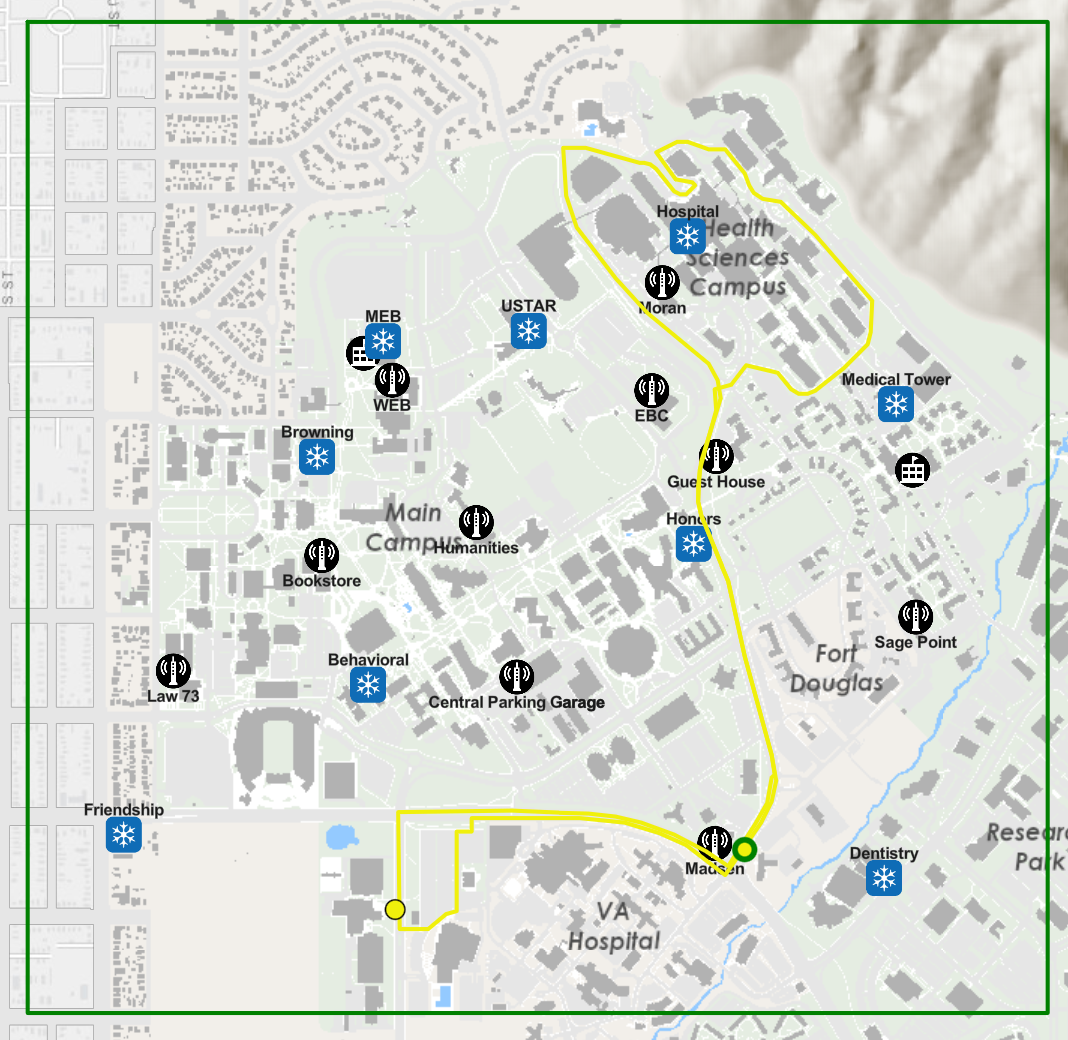
\includegraphics[width=\areaofinterestfigwidth]{figs/Guardsmen_Direct_Route_1.png}
                \caption{The ``Guardsmen Direct" route around the University of Utah campus -- to be traversed by the Rx}
                \label{fig:Rx_4}
            \end{figure}
            \begin{figure}
                \centering
                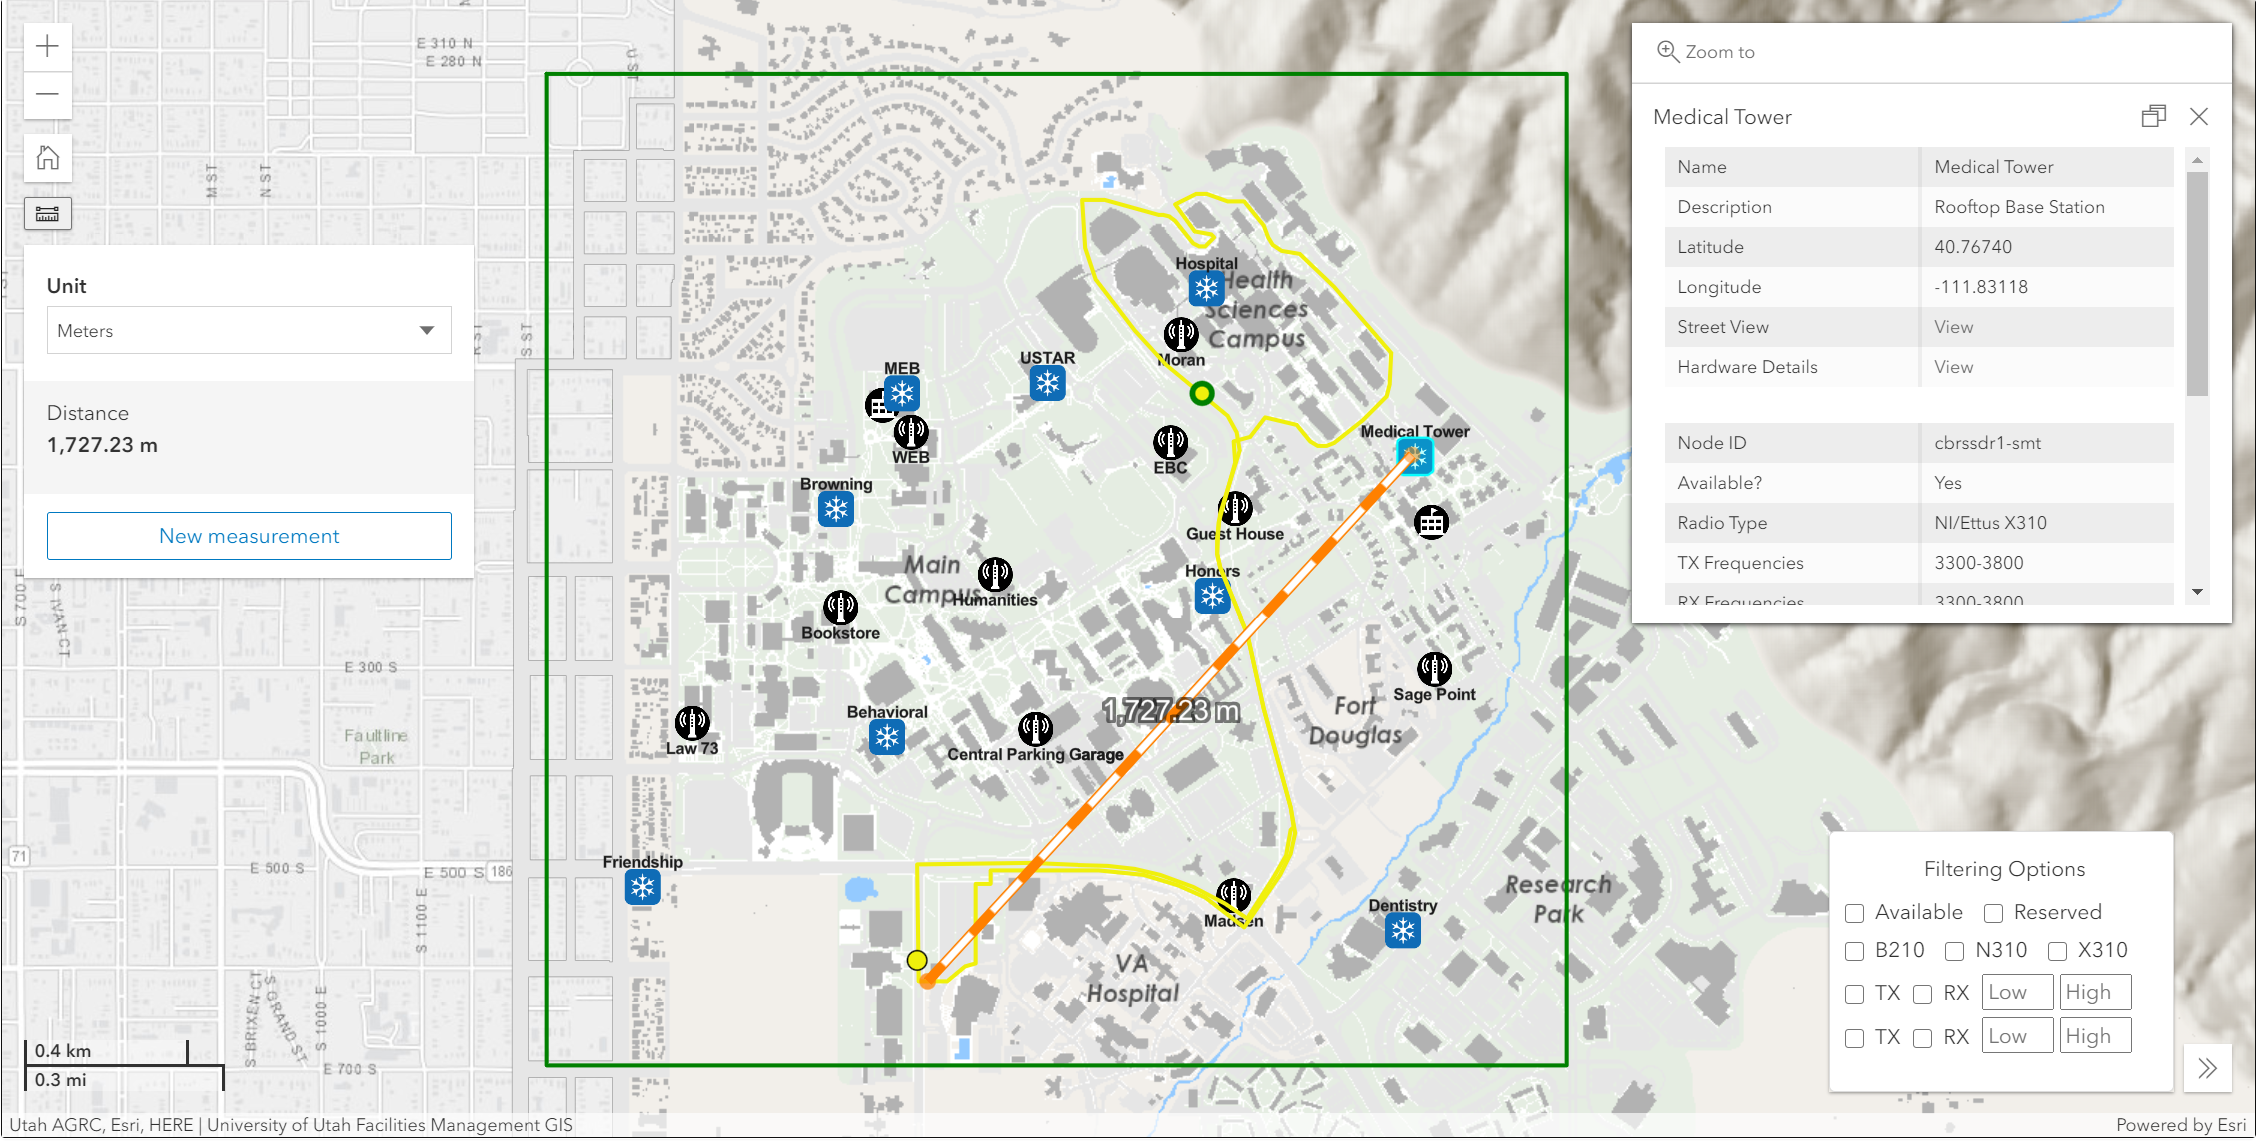
\includegraphics[width=\areaofinterestfigwidth]{figs/Guardsmen_Direct_Route_1_Medical_Tower_Tx.png}
                \caption{The location of the Tx (fixed) while the Rx moves along the ``Guardsmen Direct" route}
                \label{fig:Tx_4}
            \end{figure}
            \begin{figure}
                \centering
                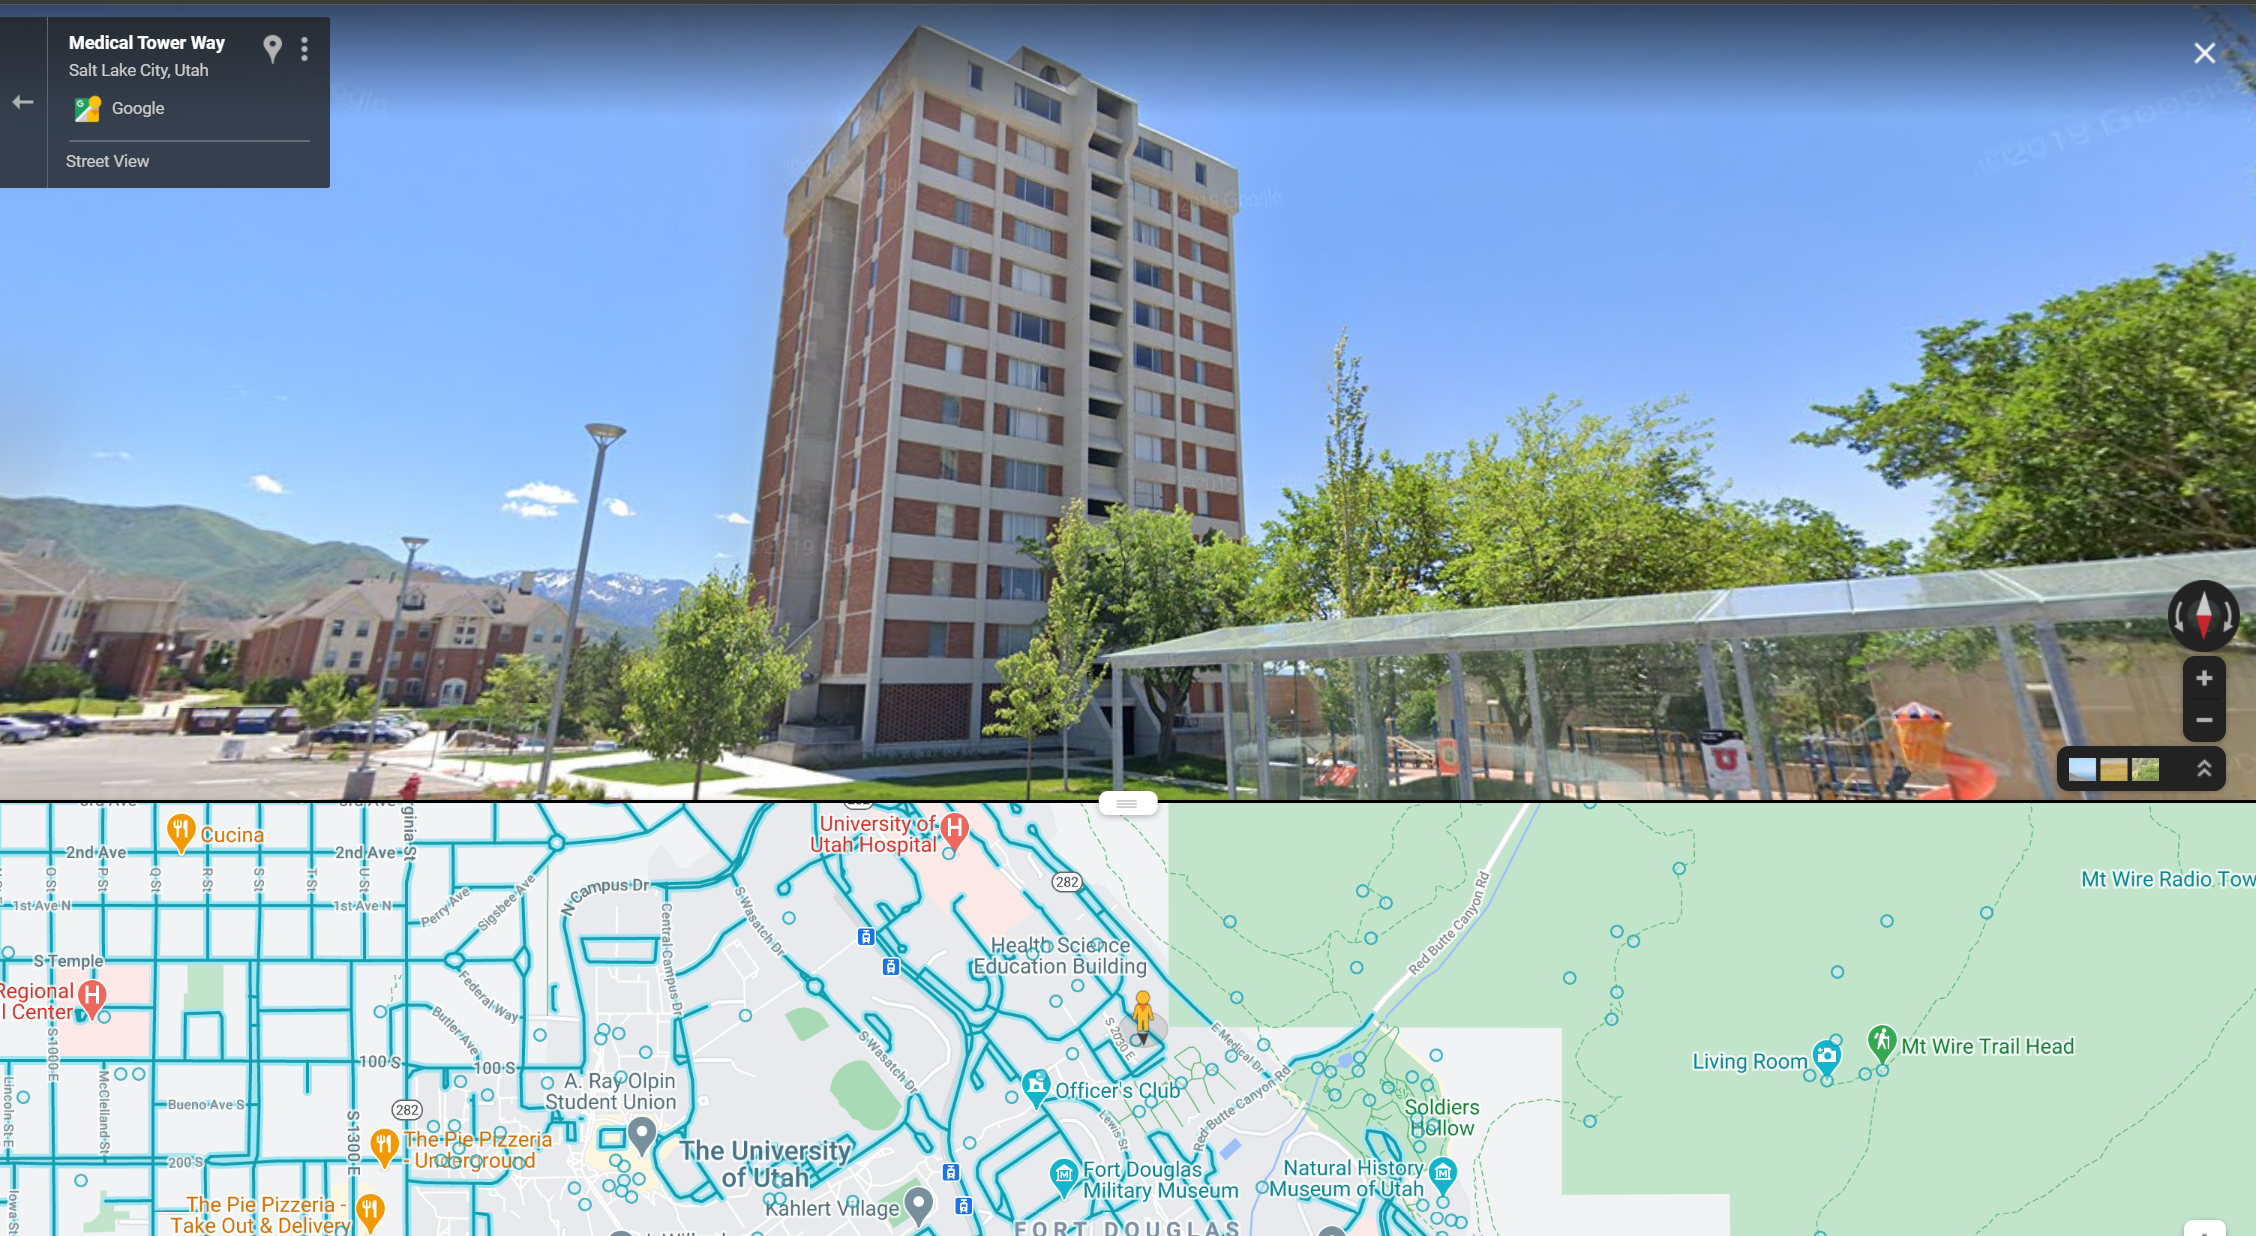
\includegraphics[width=\areaofinterestfigwidth]{figs/Medical_Tower_Tx.png}
                \caption{A street view of the Medical Tower Tx mount point for the ``Guardsmen Direct" Rx route}
                \label{fig:Tx_4_details}
            \end{figure}
            \item \underline{Guardsmen Direct}: Rx along the route depicted in \Cref{fig:Rx_4} -- with the Tx affixed at the mount-point depicted in \Cref{fig:Tx_4} and \Cref{fig:Tx_4_details} -- for site-specific mmWave propagation modeling in urban environments;
            
            \begin{figure}
                \centering
                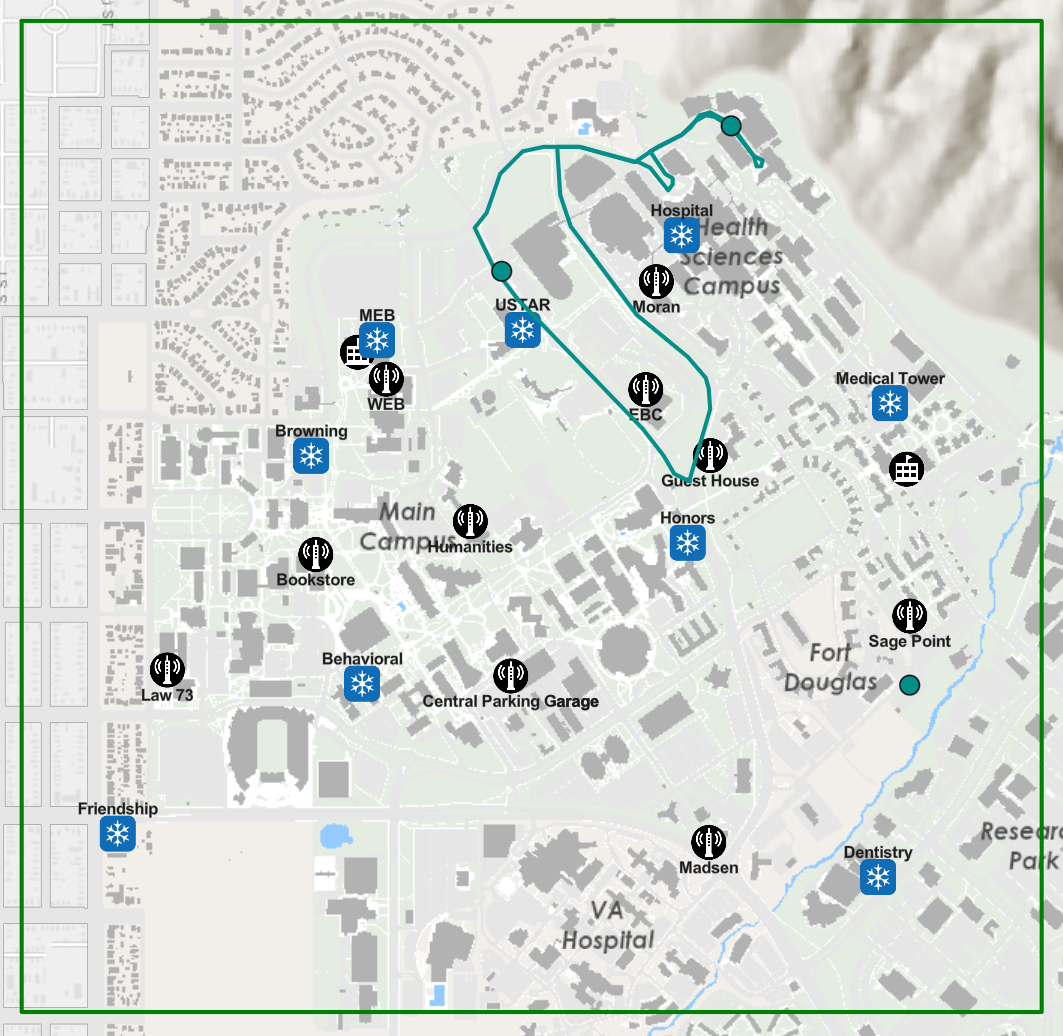
\includegraphics[width=\areaofinterestfigwidth]{figs/Wasatch_Express_Route_4.png}
                \caption{The ``Wasatch Express" route around the University of Utah campus -- to be traversed by the Rx}
                \label{fig:Rx_5}
            \end{figure}
            \begin{figure}
                \centering
                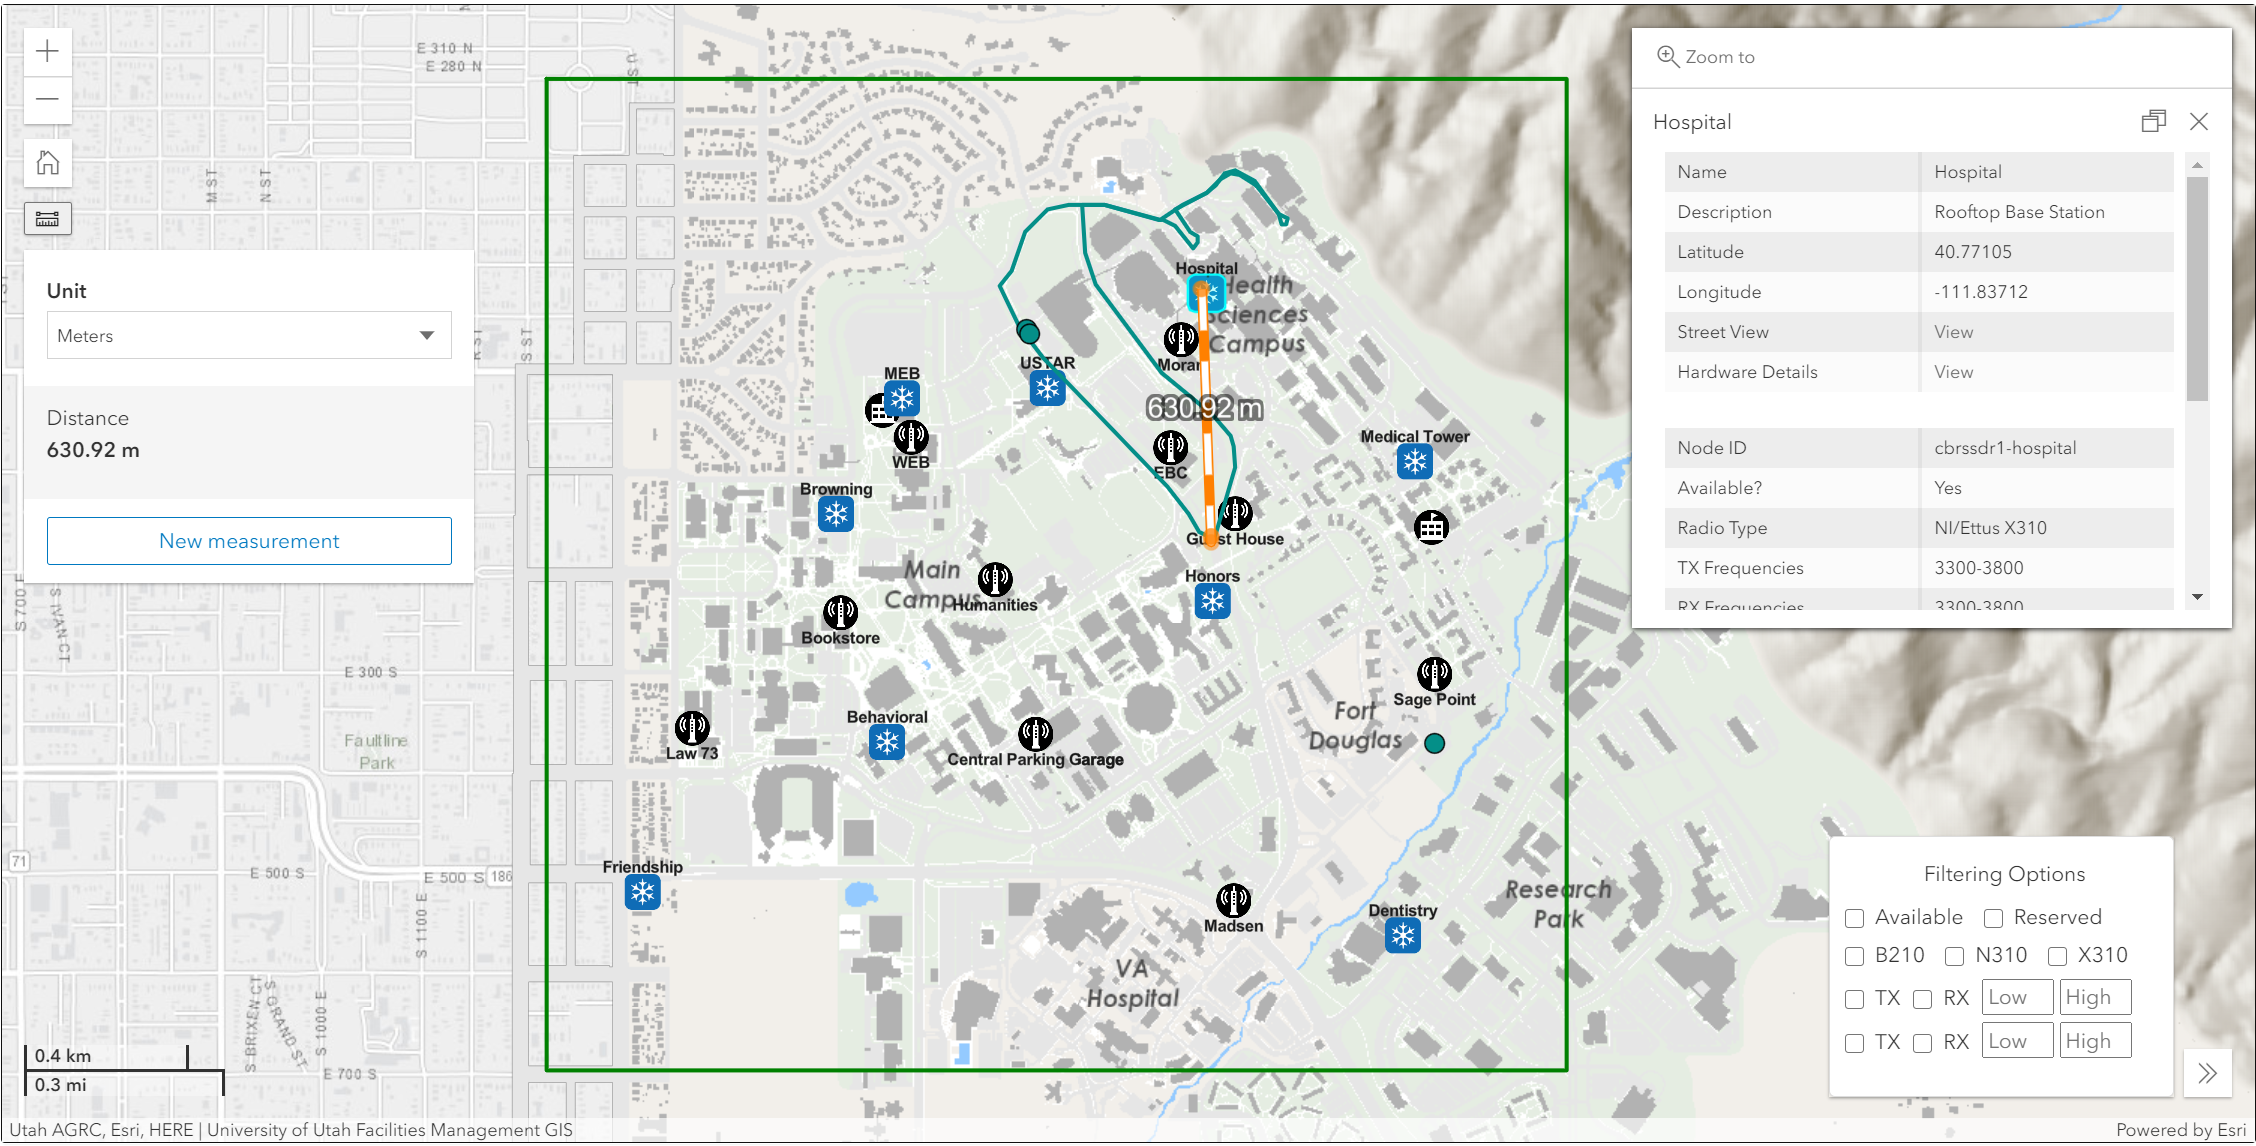
\includegraphics[width=\areaofinterestfigwidth]{figs/Wasatch_Express_Route_4_Hospital_Tx.png}
                \caption{The location of the Tx (fixed) while the Rx moves along the ``Wasatch Express" route}
                \label{fig:Tx_5}
            \end{figure}
            \begin{figure}
                \centering
                \includegraphics[width=\areaofinterestfigwidth]{figs/Hospital_Tx.png}
                \caption{A street view of the University of Utah Hospital Building Tx mount point for the ``Wasatch Express" Rx route}
                \label{fig:Tx_5_details}
            \end{figure}
            \item \underline{Wasatch Express}: Rx along the route depicted in \Cref{fig:Rx_5} -- with the Tx affixed at the mount-point depicted in \Cref{fig:Tx_5} and \Cref{fig:Tx_5_details} -- for site-specific mmWave propagation modeling in urban environments; and
            
            \begin{figure}
                \centering
                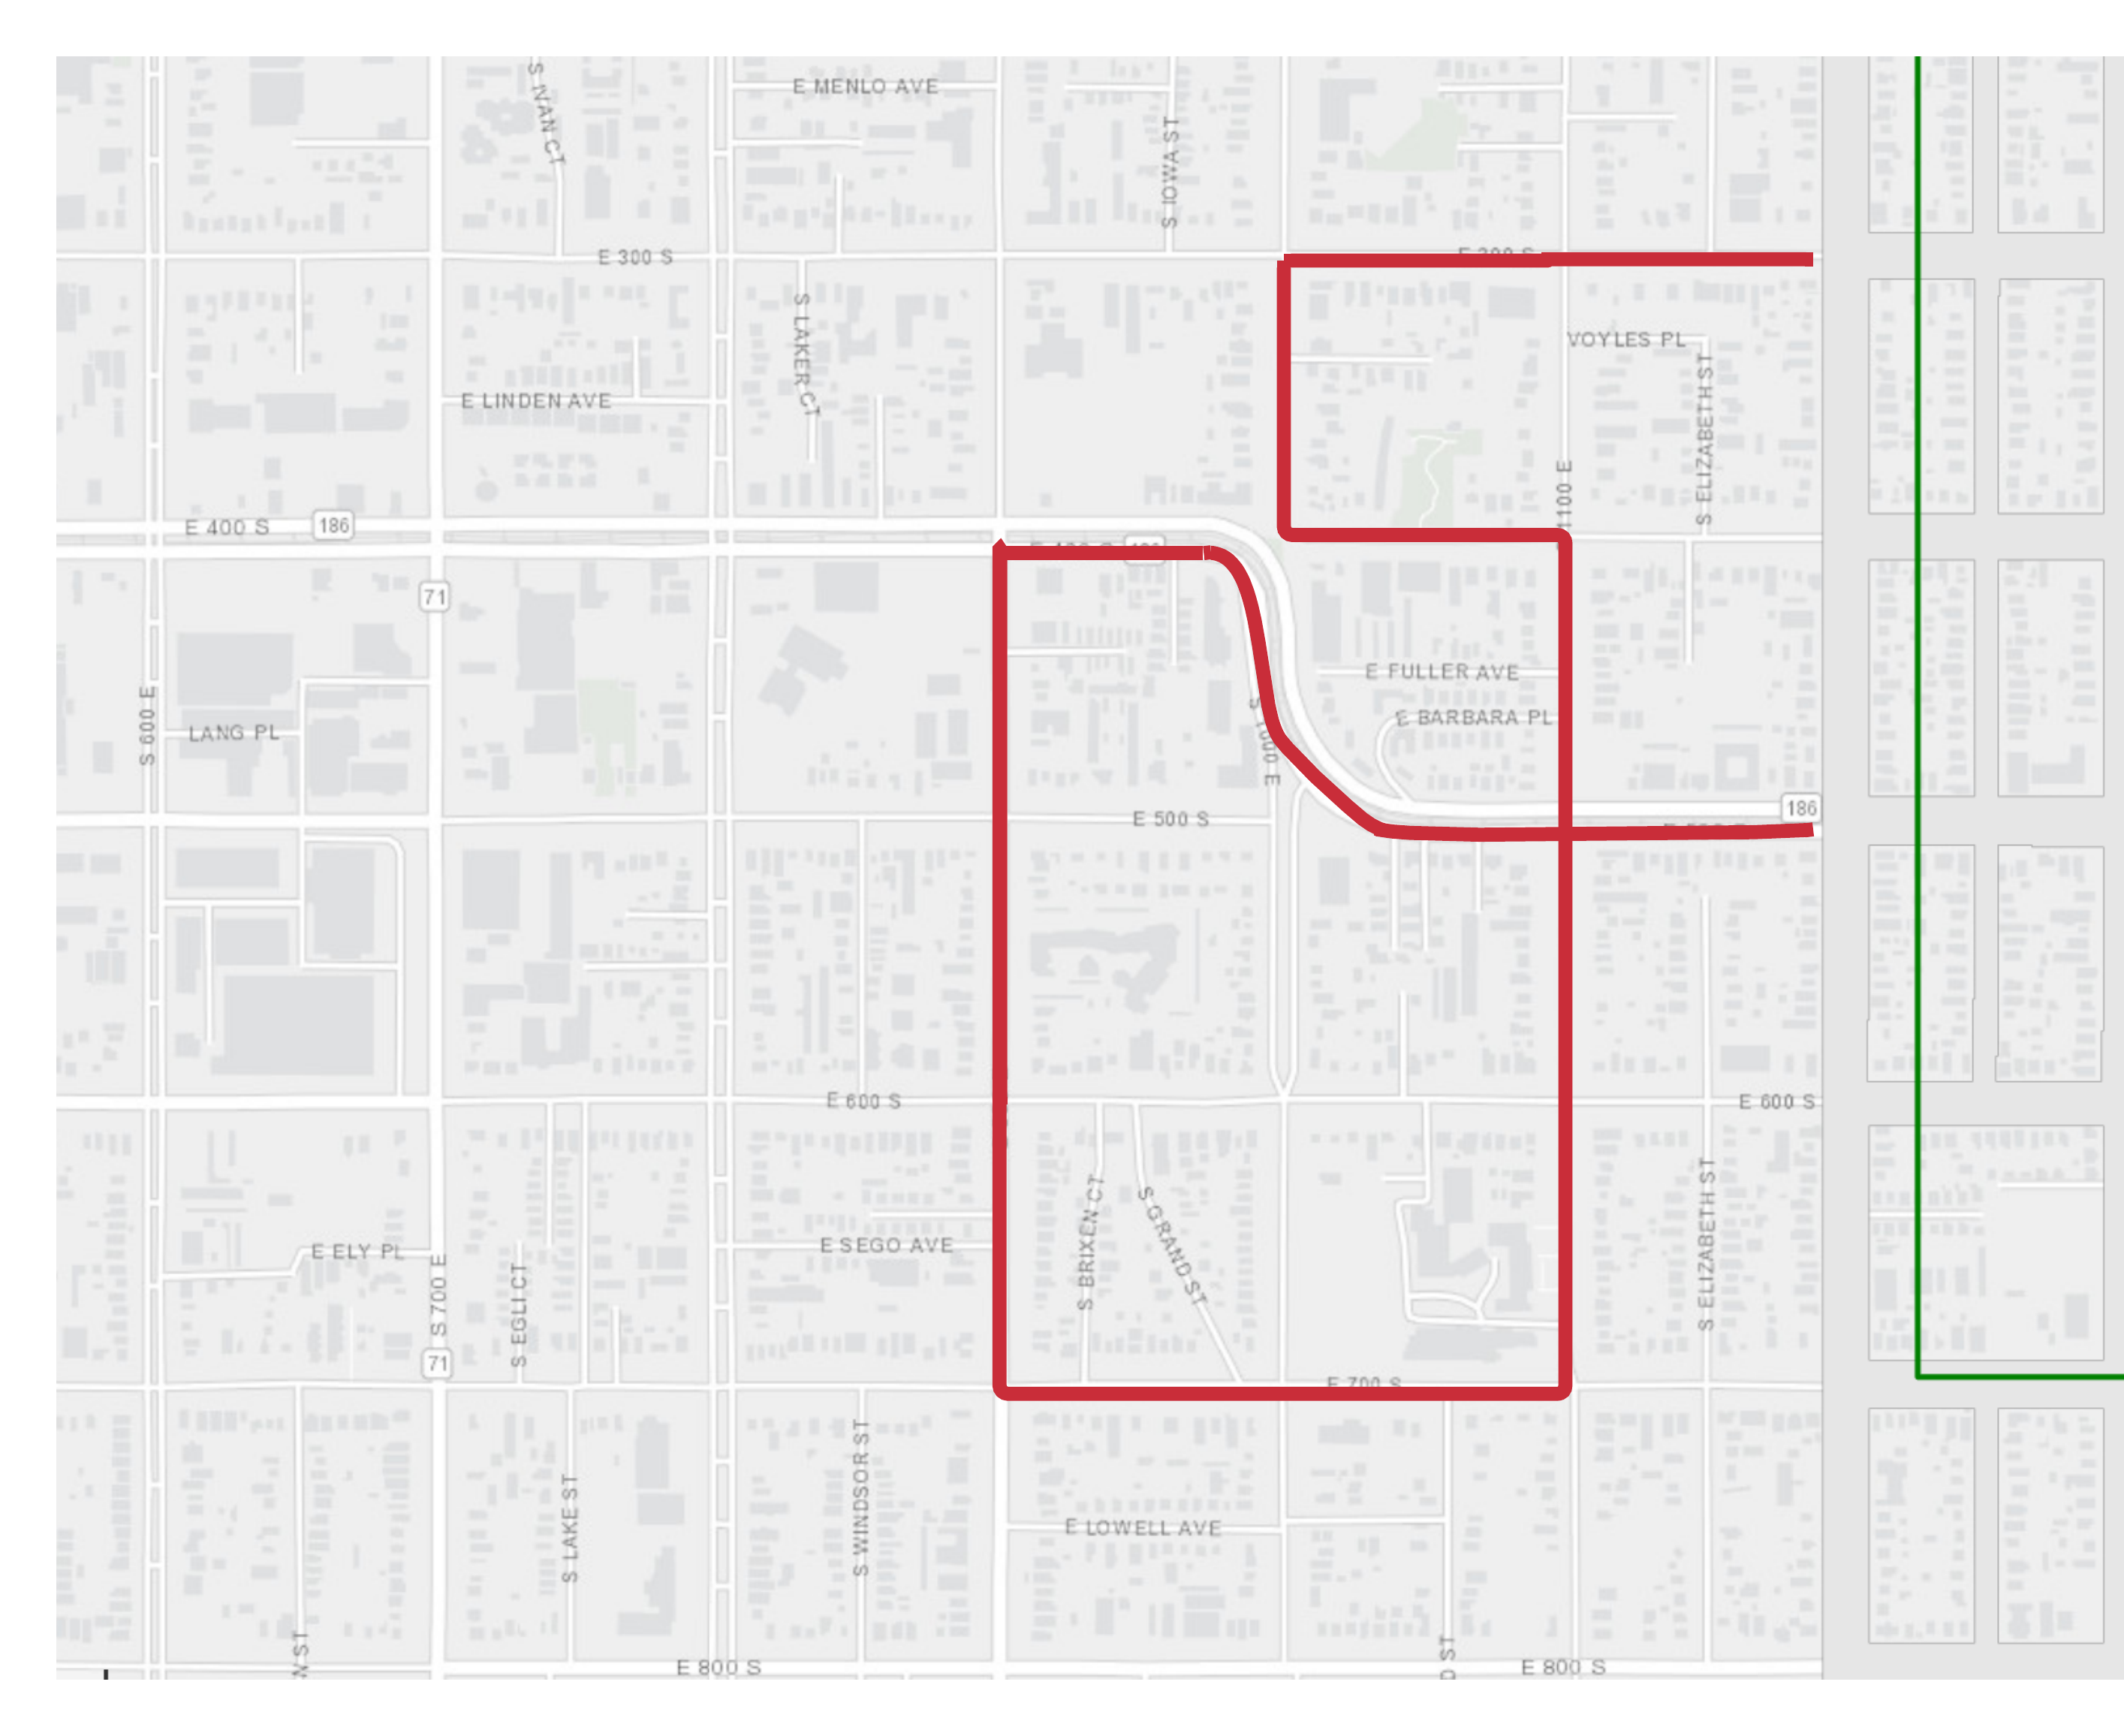
\includegraphics[width=\areaofinterestfigwidth]{figs/Suburban_Route_6_Zoomed.png}
                \caption{The ``Suburban" route around the University of Utah campus -- to be traversed by the Rx}
                \label{fig:Rx_6}
            \end{figure}
            \begin{figure}
                \centering
                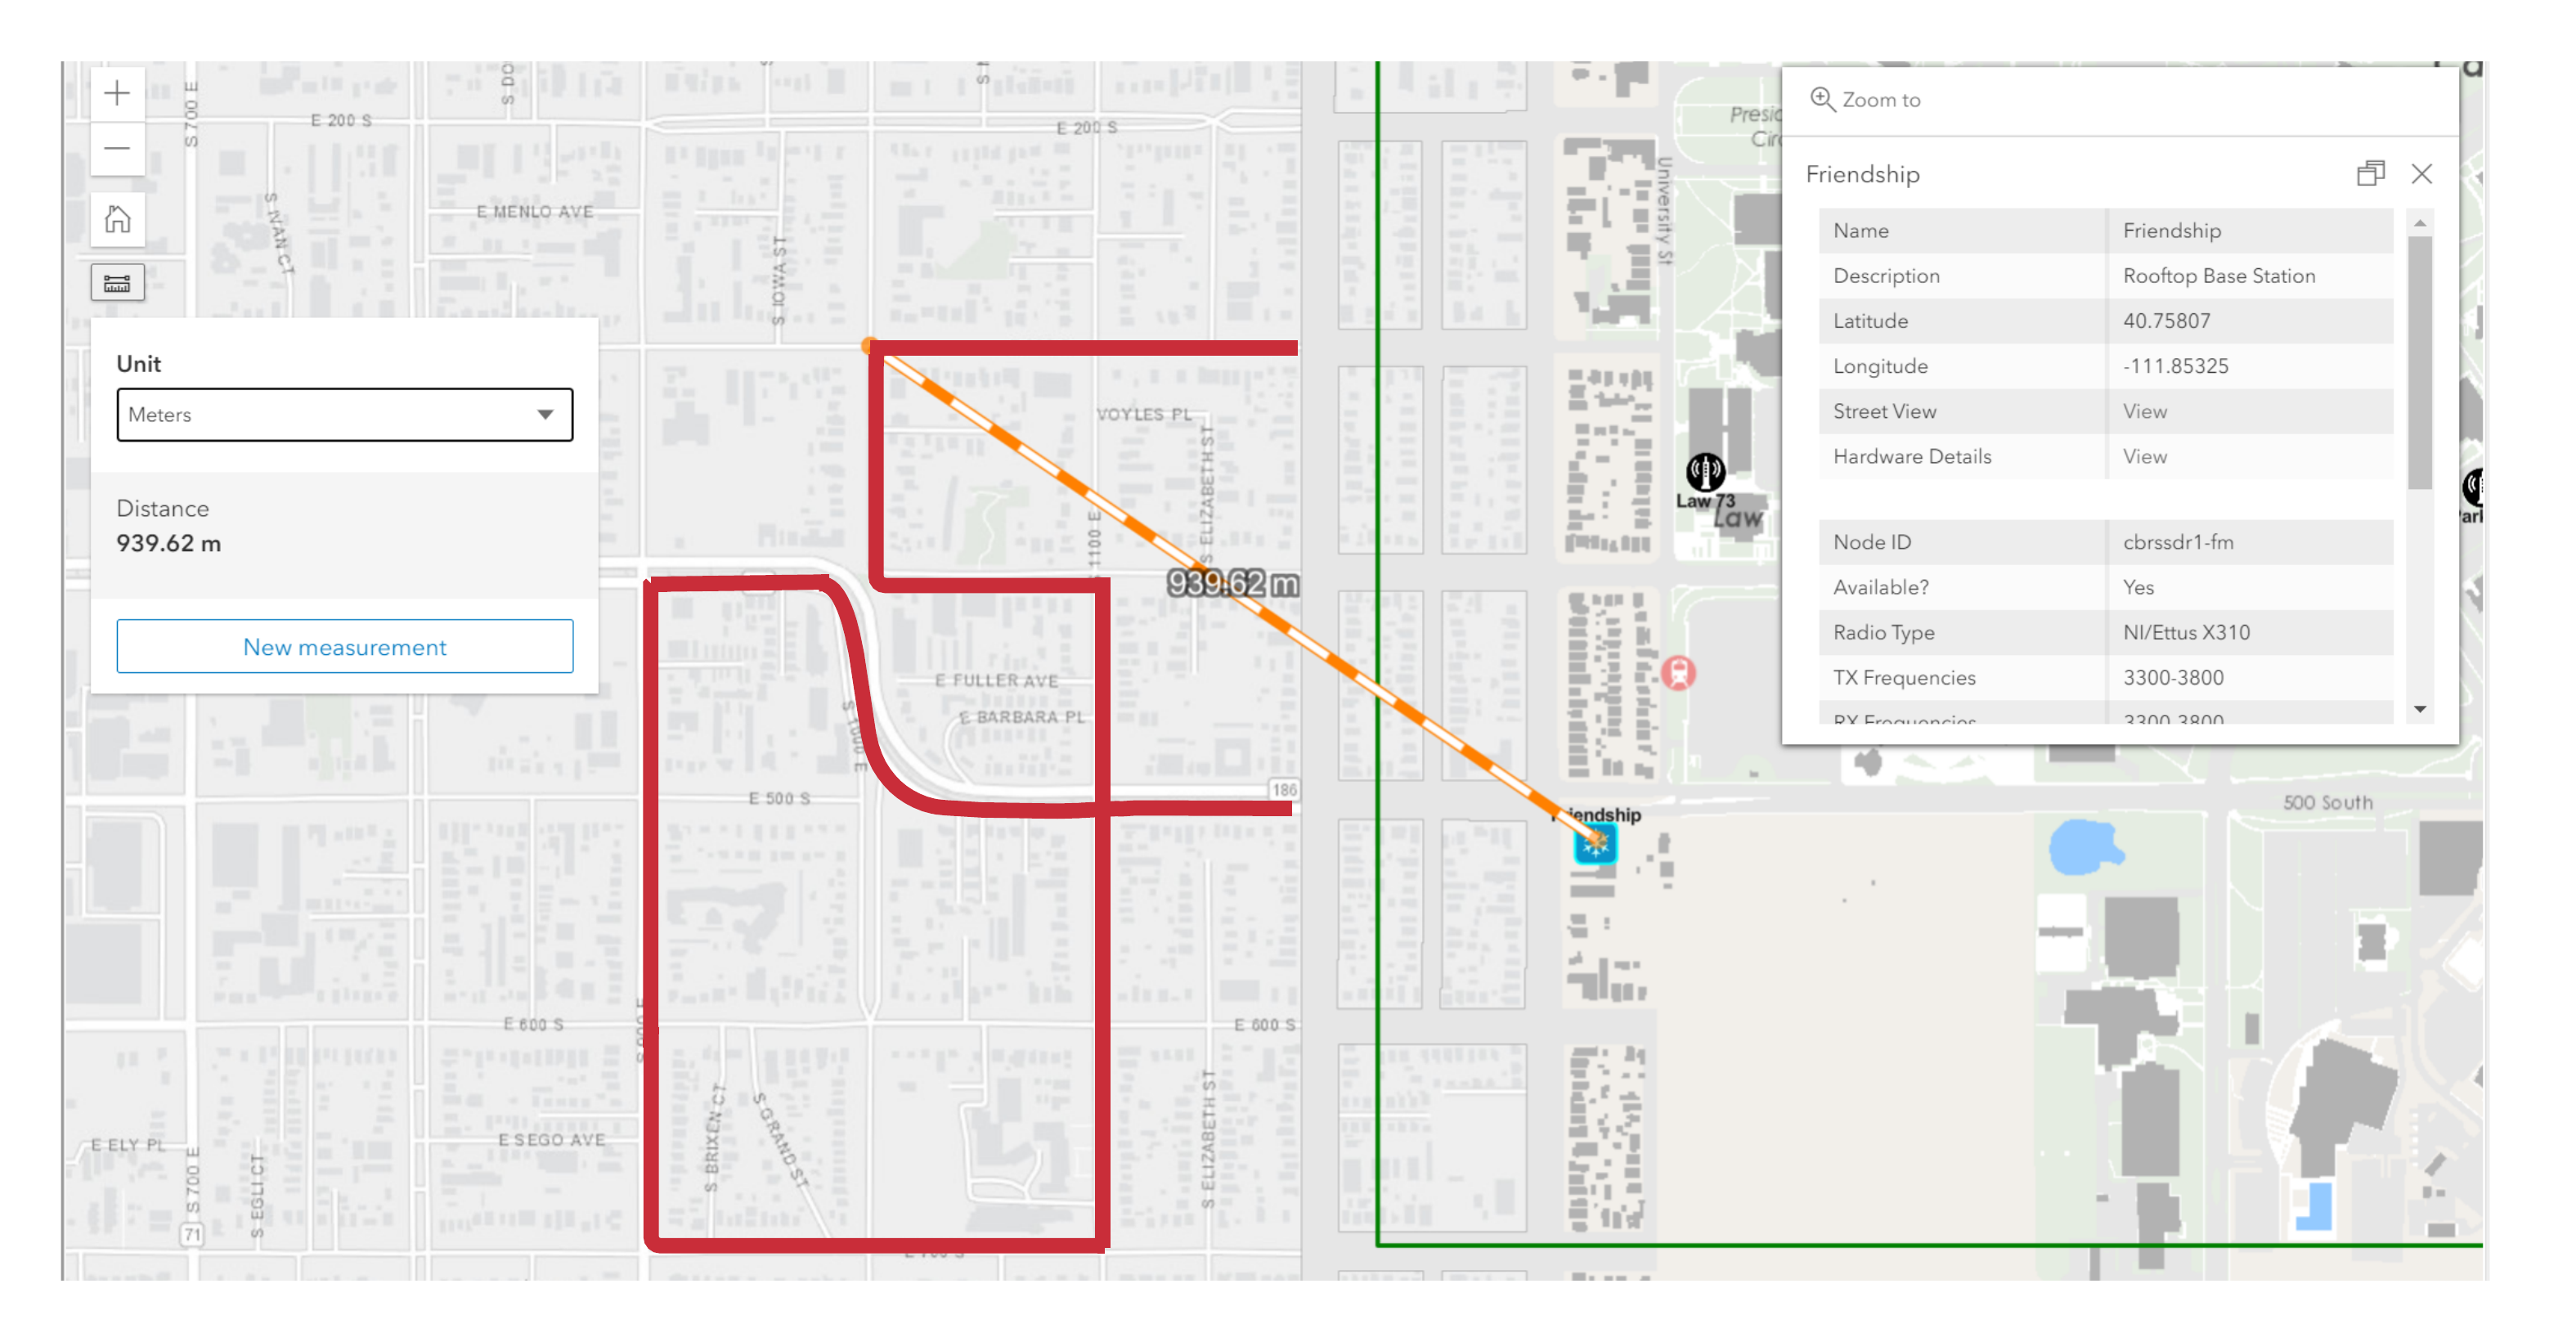
\includegraphics[width=\areaofinterestfigwidth]{figs/Suburban_Route_6_Friendship_Tx.png}
                \caption{The location of the Tx (fixed) while the Rx moves along the ``Suburban" route}
                \label{fig:Tx_6}
            \end{figure}
            \begin{figure}
                \centering
                \includegraphics[width=\areaofinterestfigwidth]{figs/Friendship_Tx.png}
                \caption{A street view of the Friendship Manor Tx mount point for the ``Suburban" Rx route}
                \label{fig:Tx_6_details}
            \end{figure}
            \begin{figure}
                \centering
                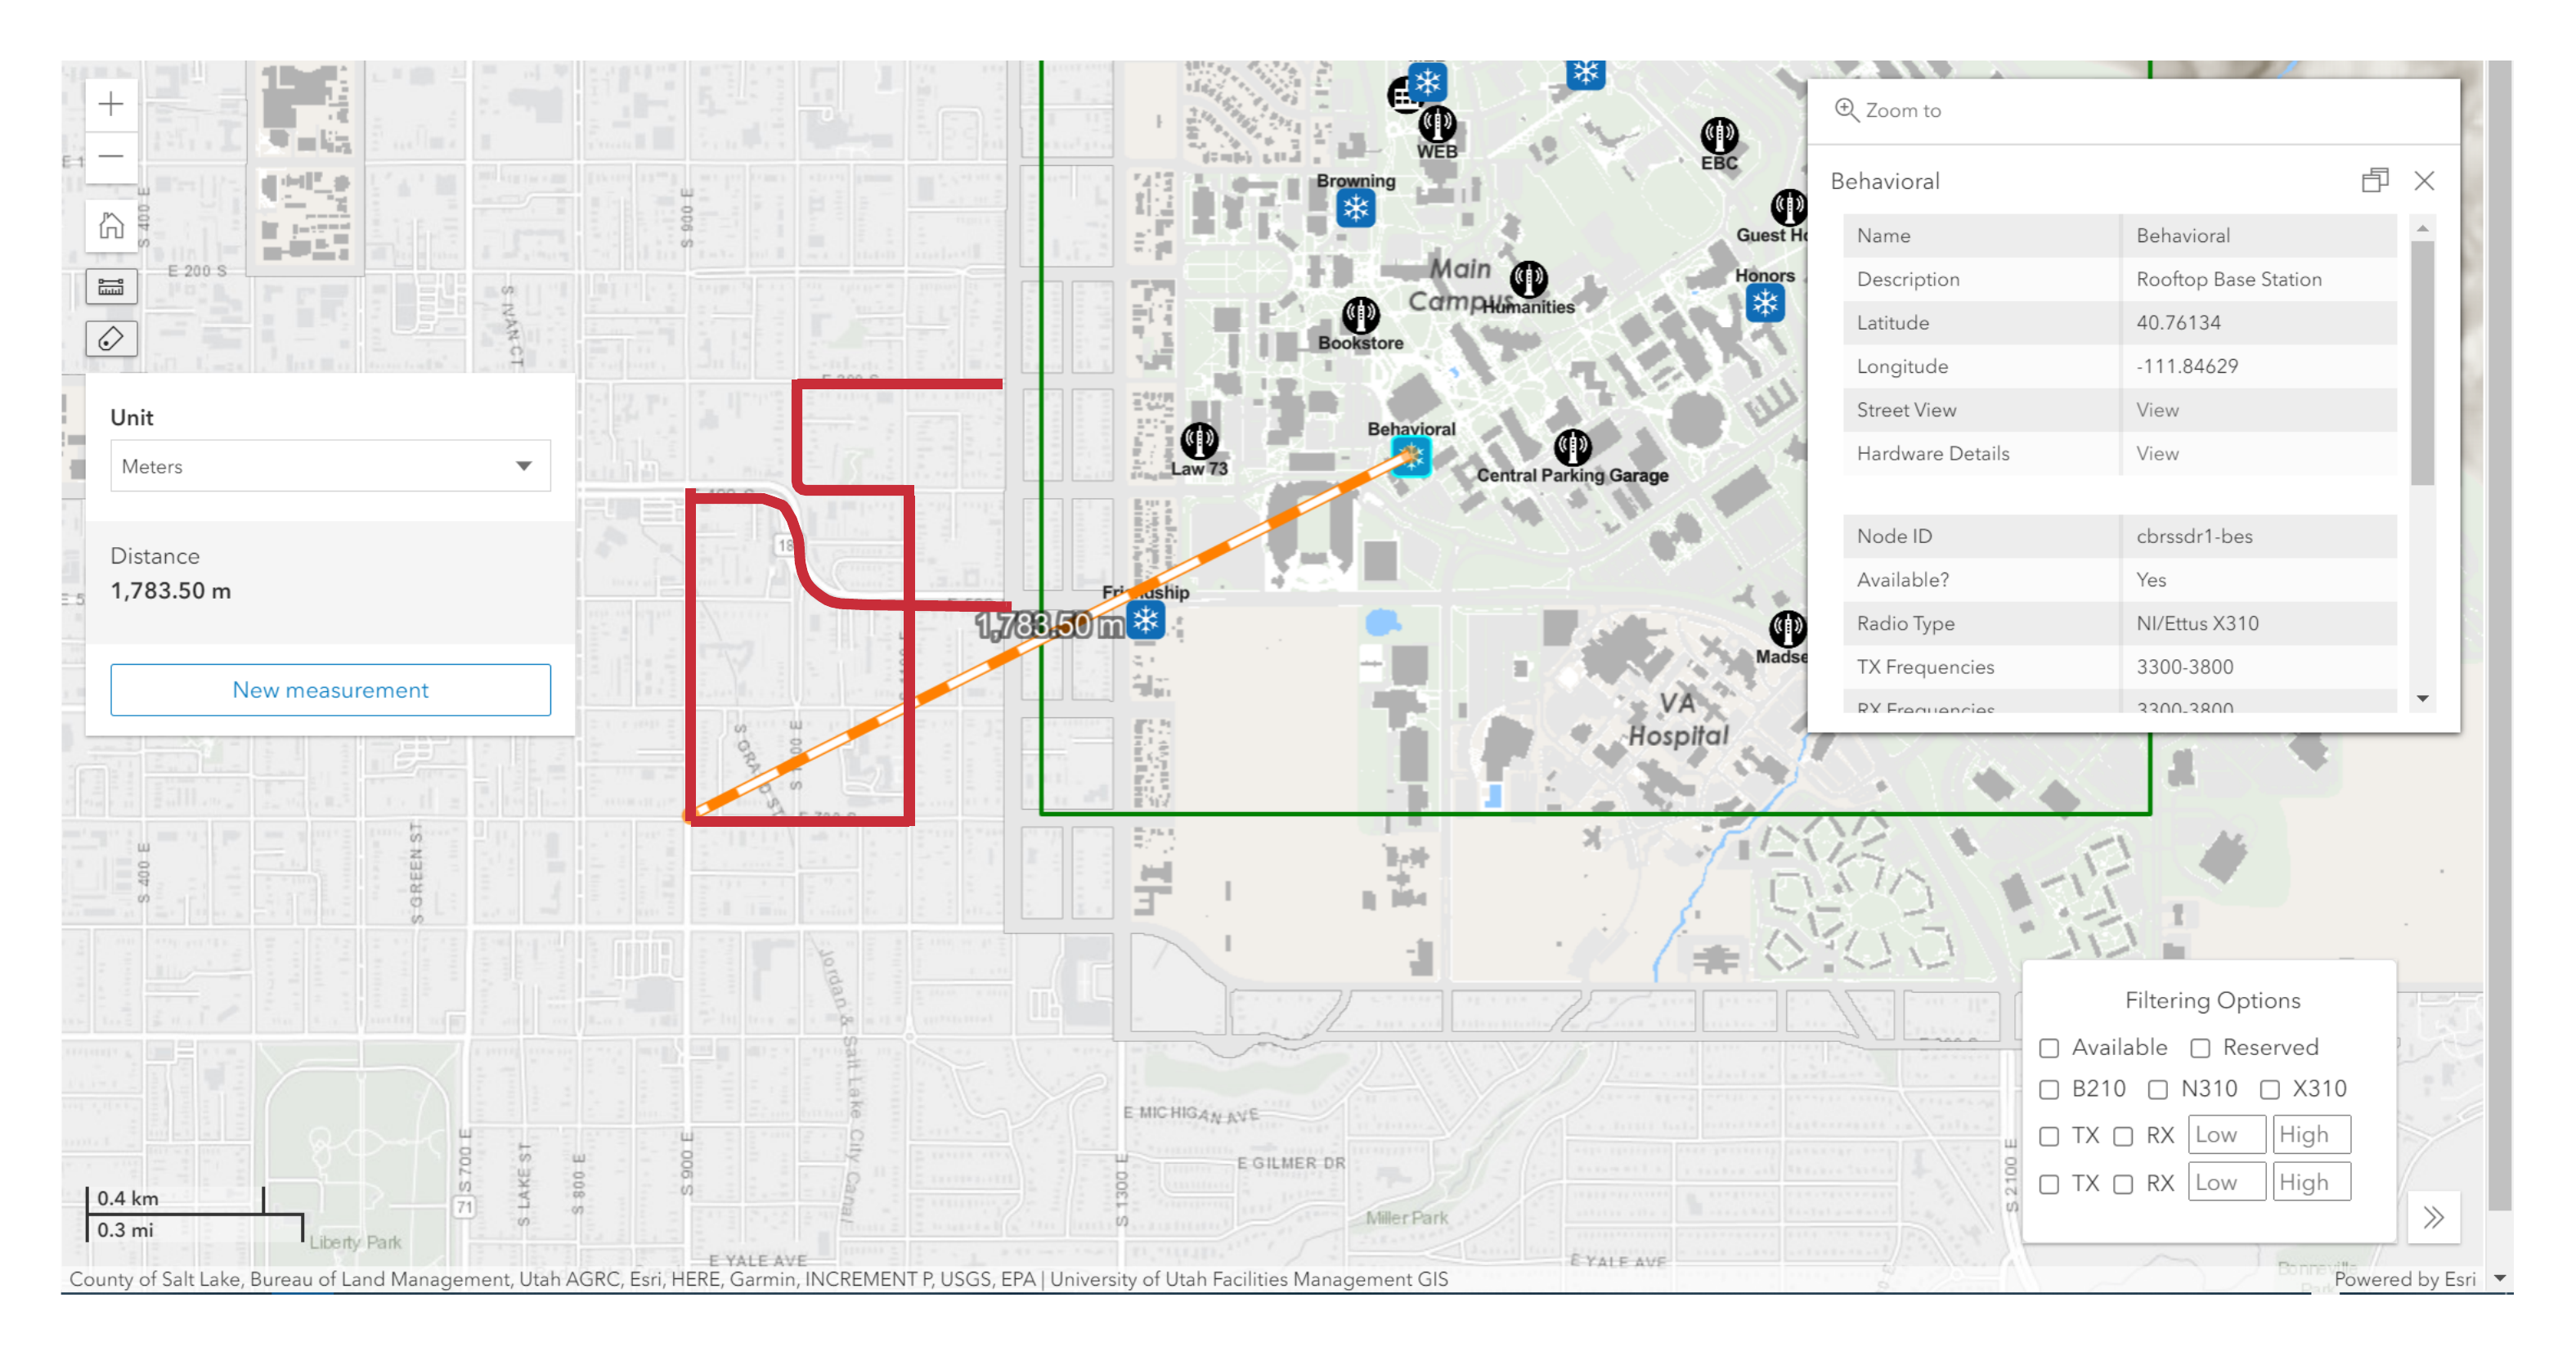
\includegraphics[width=\areaofinterestfigwidth]{figs/Suburban_Route_6_Behavioral_Tx.png}
                \caption{The location of the Tx (fixed) while the Rx moves along the ``Suburban" route}
                \label{fig:Tx_6a}
            \end{figure}
            \begin{figure}
                \centering
                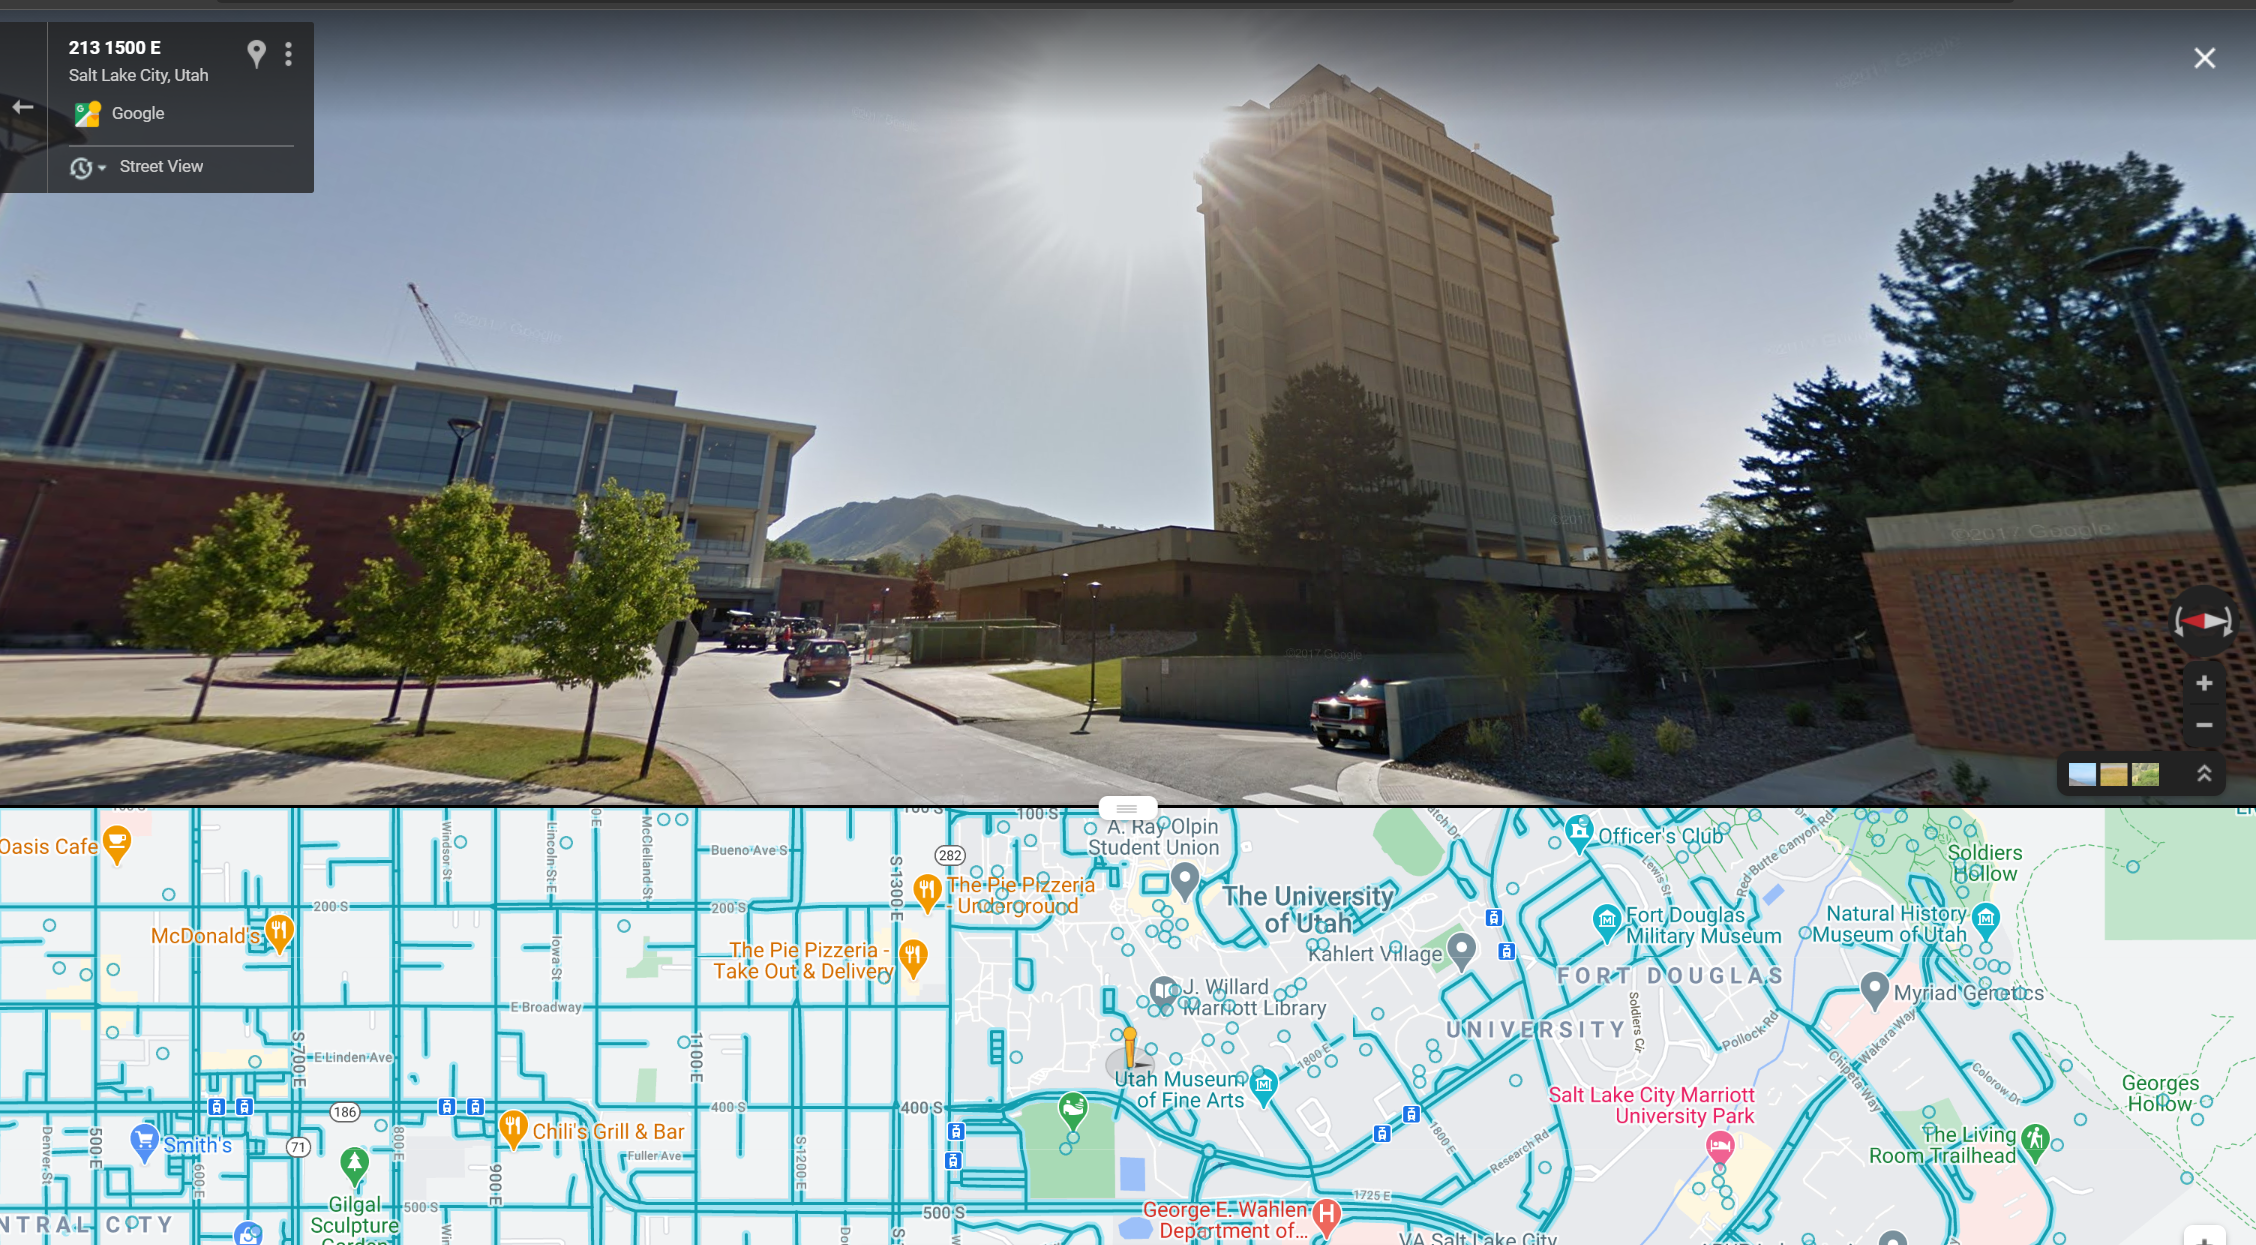
\includegraphics[width=\areaofinterestfigwidth]{figs/Behavioral_Tx.png}
                \caption{A street view of the Behavioral Sciences Building Tx mount point for the ``Suburban" Rx route}
                \label{fig:Tx_6a_details}
            \end{figure}
            \item \underline{Suburban}: Rx along the route depicted in \Cref{fig:Rx_6} -- with the Tx affixed at the mount-point depicted in \Cref{fig:Tx_6} and \Cref{fig:Tx_6_details} -- for site-specific mmWave propagation modeling in suburban environments.
        \end{itemize}
        
    \subsection{Rx Chosen Routes}\label{S3.4}
    Of the potential Rx route candidates listed in Sec. \ref{S3.3}, based on our internal discussions, we have decided to use the ``Blue Detour" route for urban measurements and the ``Suburban" route for suburban measurements. As a result, the corresponding Tx mount points are chosen to be the roof-top of the University of Utah Hospital building (for the ``Blue Detour" route) and the roof-top of the Behavioral Sciences building (for the ``Suburban" route).\newline
    
    \noindent The other routes listed in Sec. \ref{S3.3} will serve as backups in case we encounter unforeseen circumstances during our measurement runs along the chosen routes.
    
    \subsection{Resource Availability and Provisioning}
        A detailed list of roof-top base-stations, near-edge computing resources (at the Fort Douglas datacenter), and Emulab compute nodes -- along with their availabilities during our measurement campaign ($8$-June-$2021$ to $18$-June-$2021$) is provided in \Cref{fig:avail}.\newline
        
        \noindent As of writing this measurement plan, we do not intend to use the USRP radios available at the various Tx mount-point candidates (Sec. \ref{S3.2}), i.e., the fixed end-points and roof-top base-stations; instead, we would be leveraging the flexible BYOD capabilities of the POWDER testbed by integrating an internally developed $28$GHz communication system (detailed in Sec. \ref{S3.5}) with our autonomous antenna tracking system (Sec. \ref{S3.6}). However, we plan to provision compute nodes -- either near-edge computing resources or compute nodes from the Emulab/Cloudlab clusters -- for fault-tolerant data storage, global system installations, centralized coordination of our Tx and Rx autonomous antenna rotating platforms (via Docker, Apache Zookeeper, Apache Kafka, and RPyC distributed control), and to handle offloaded processing tasks from our Tx and Rx end-points. As a result, resource provisioning scripts have been written to orchestrate the following capabilities: node (and Linux image) provisioning, package installations, startup shell script executions, and SCM clones (main repository and sub-modules). A sample Python script involving a geni-lib resource request for a Dell PowerEdge R740 server (d740 near-edge compute resource) is shown in \Cref{fig:profile}.\newline
        
        \noindent As mentioned earlier, our Rx autonomous antenna tracking platform along with its $28$GHz communication setup, would be mounted on a van and driven around the University of Utah along pre-determined routes (Sec. \ref{S3.4}); while our Tx autonomous antenna tracking platform along with its $28$GHz communication setup, would be affixed atop suitable route-specific mount-points (Sec. \ref{S3.4}).\newline
        
        \noindent During a particular run of this measurement campaign, both the Tx and Rx antenna tracking platforms log their IMU (pan \& tilt) and GPS (NMEA-JSON) measurements locally -- along with distributed, redundant storage at the provisioned compute nodes, facilitated by Apache Kafka; additionally, time-stamped power delay profile samples (swept at $2.5$GHz at the Rx) would be logged onto the file-system of an Rx-mounted Raspberry Pi via a USRP B$200$mini GNURadio implementation -- which would be published to the aforementioned fault-tolerant Apache Kafka message-oriented middleware framework.
        \begin{figure}
            \centering
            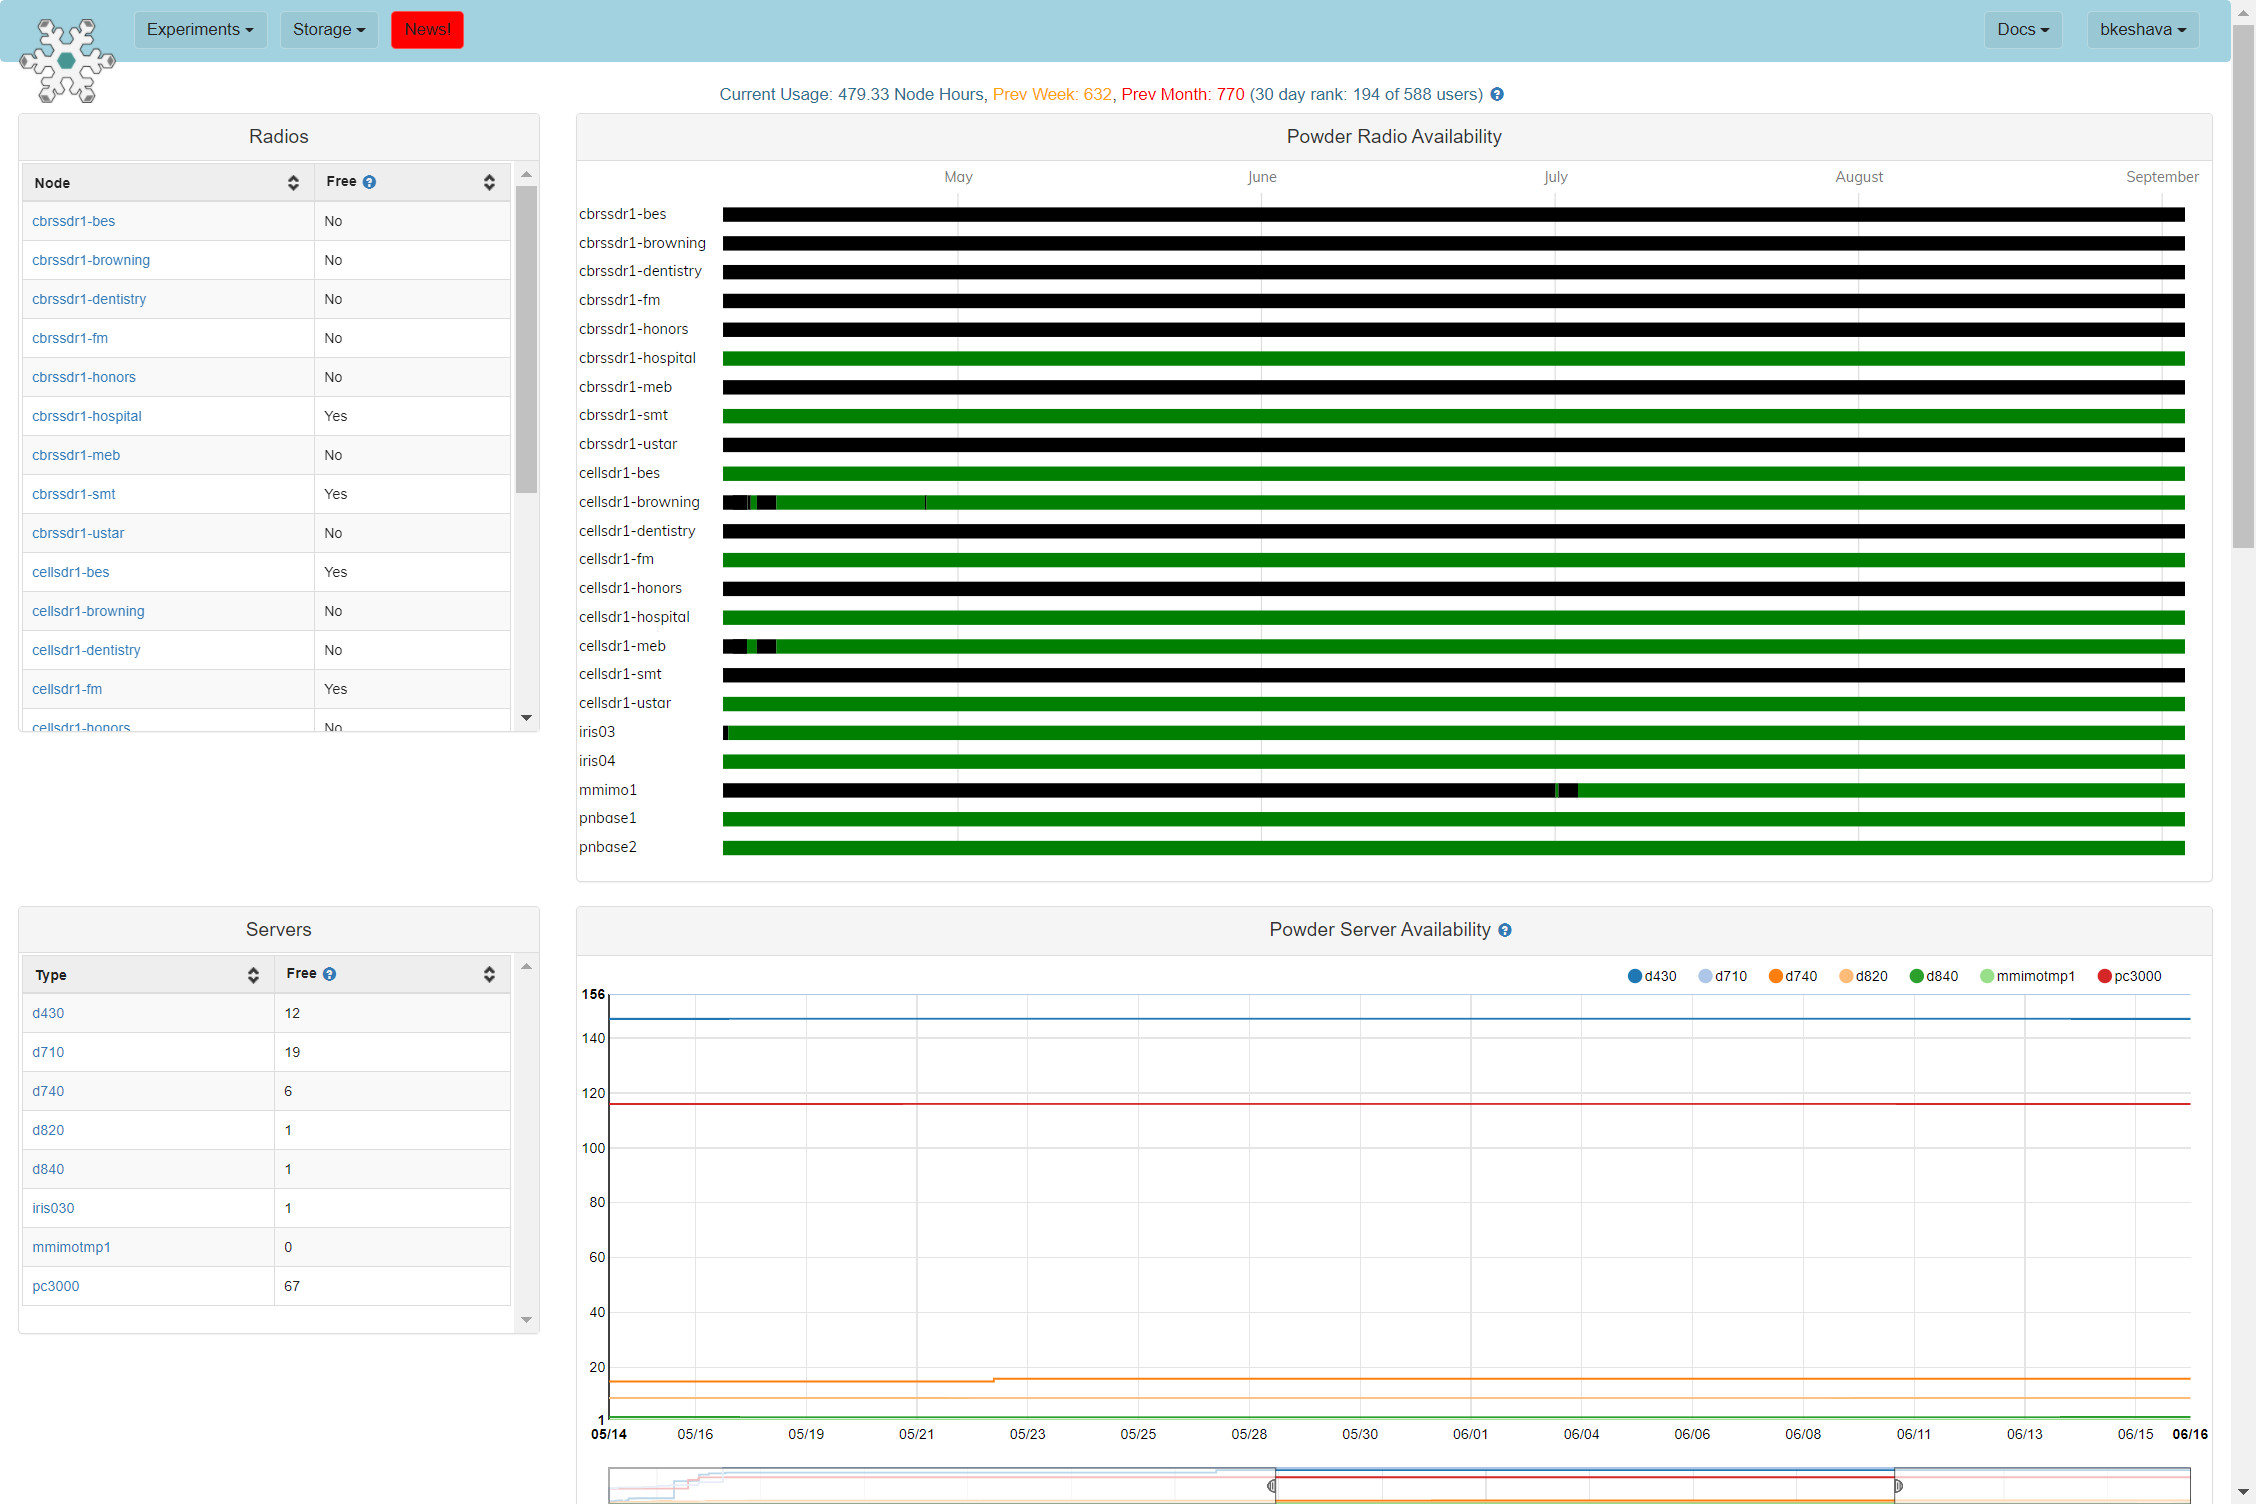
\includegraphics[width=\areaofinterestfigwidth]{figs/POWDER_Resource_Availability.png}
            \caption{A list of radio and compute resources available on the University of Utah's POWDER testbed}
            \label{fig:avail}
        \end{figure}
        \begin{figure}
            \centering
            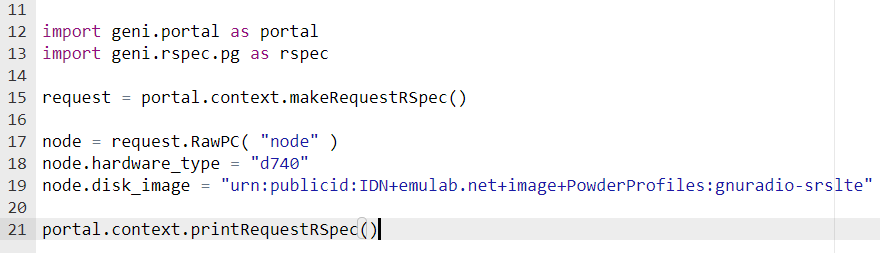
\includegraphics[width=\areaofinterestfigwidth]{figs/Resource_Provisioning.png}
            \caption{A resource-provisioning script (Python/geni-lib/RSpec) incorporated within a newly-instantiated POWDER profile}
            \label{fig:profile}
        \end{figure}
    
    \begin{figure}
        \centering
        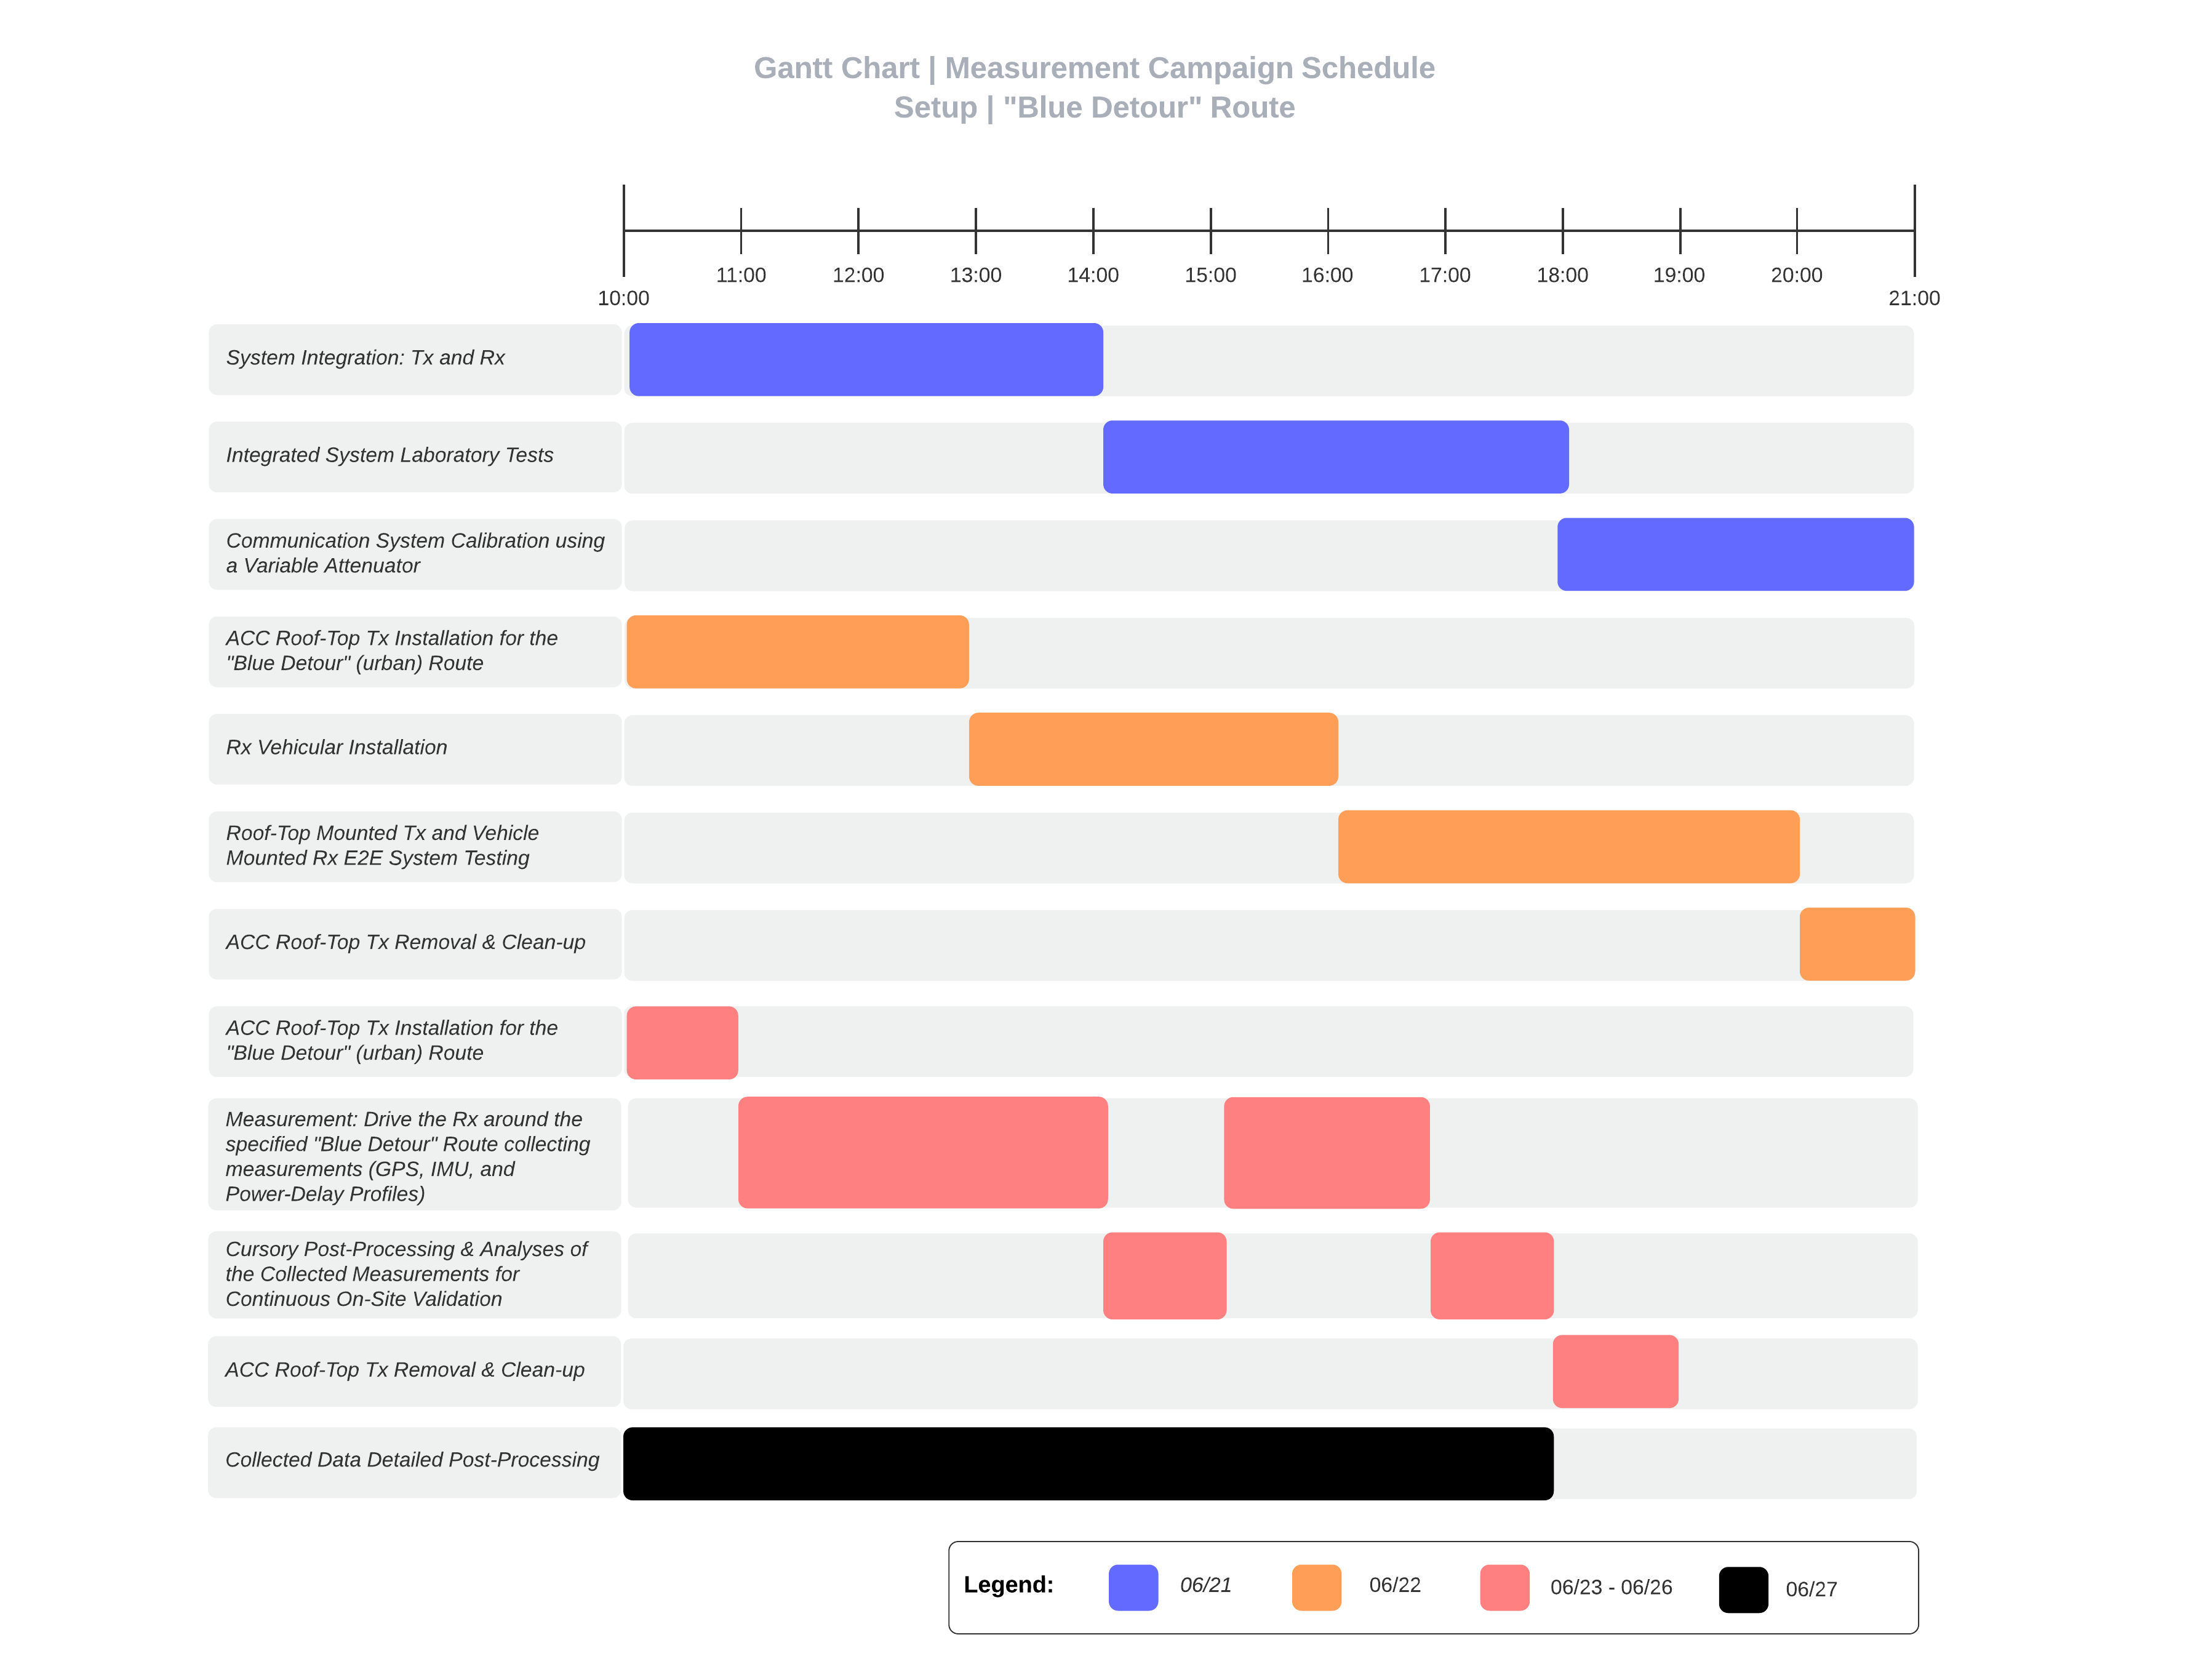
\includegraphics[width=\areaofinterestfigwidth]{figs/Odin_Measurement_Campaign_Schedule_Urban.png}
        \caption{A Gantt chart detailing our timelines for system setup -- in addition to our plans for data collection along the ``Blue Detour" route}
        \label{fig:gantt-urban}
    \end{figure}
    \begin{figure}
        \centering
        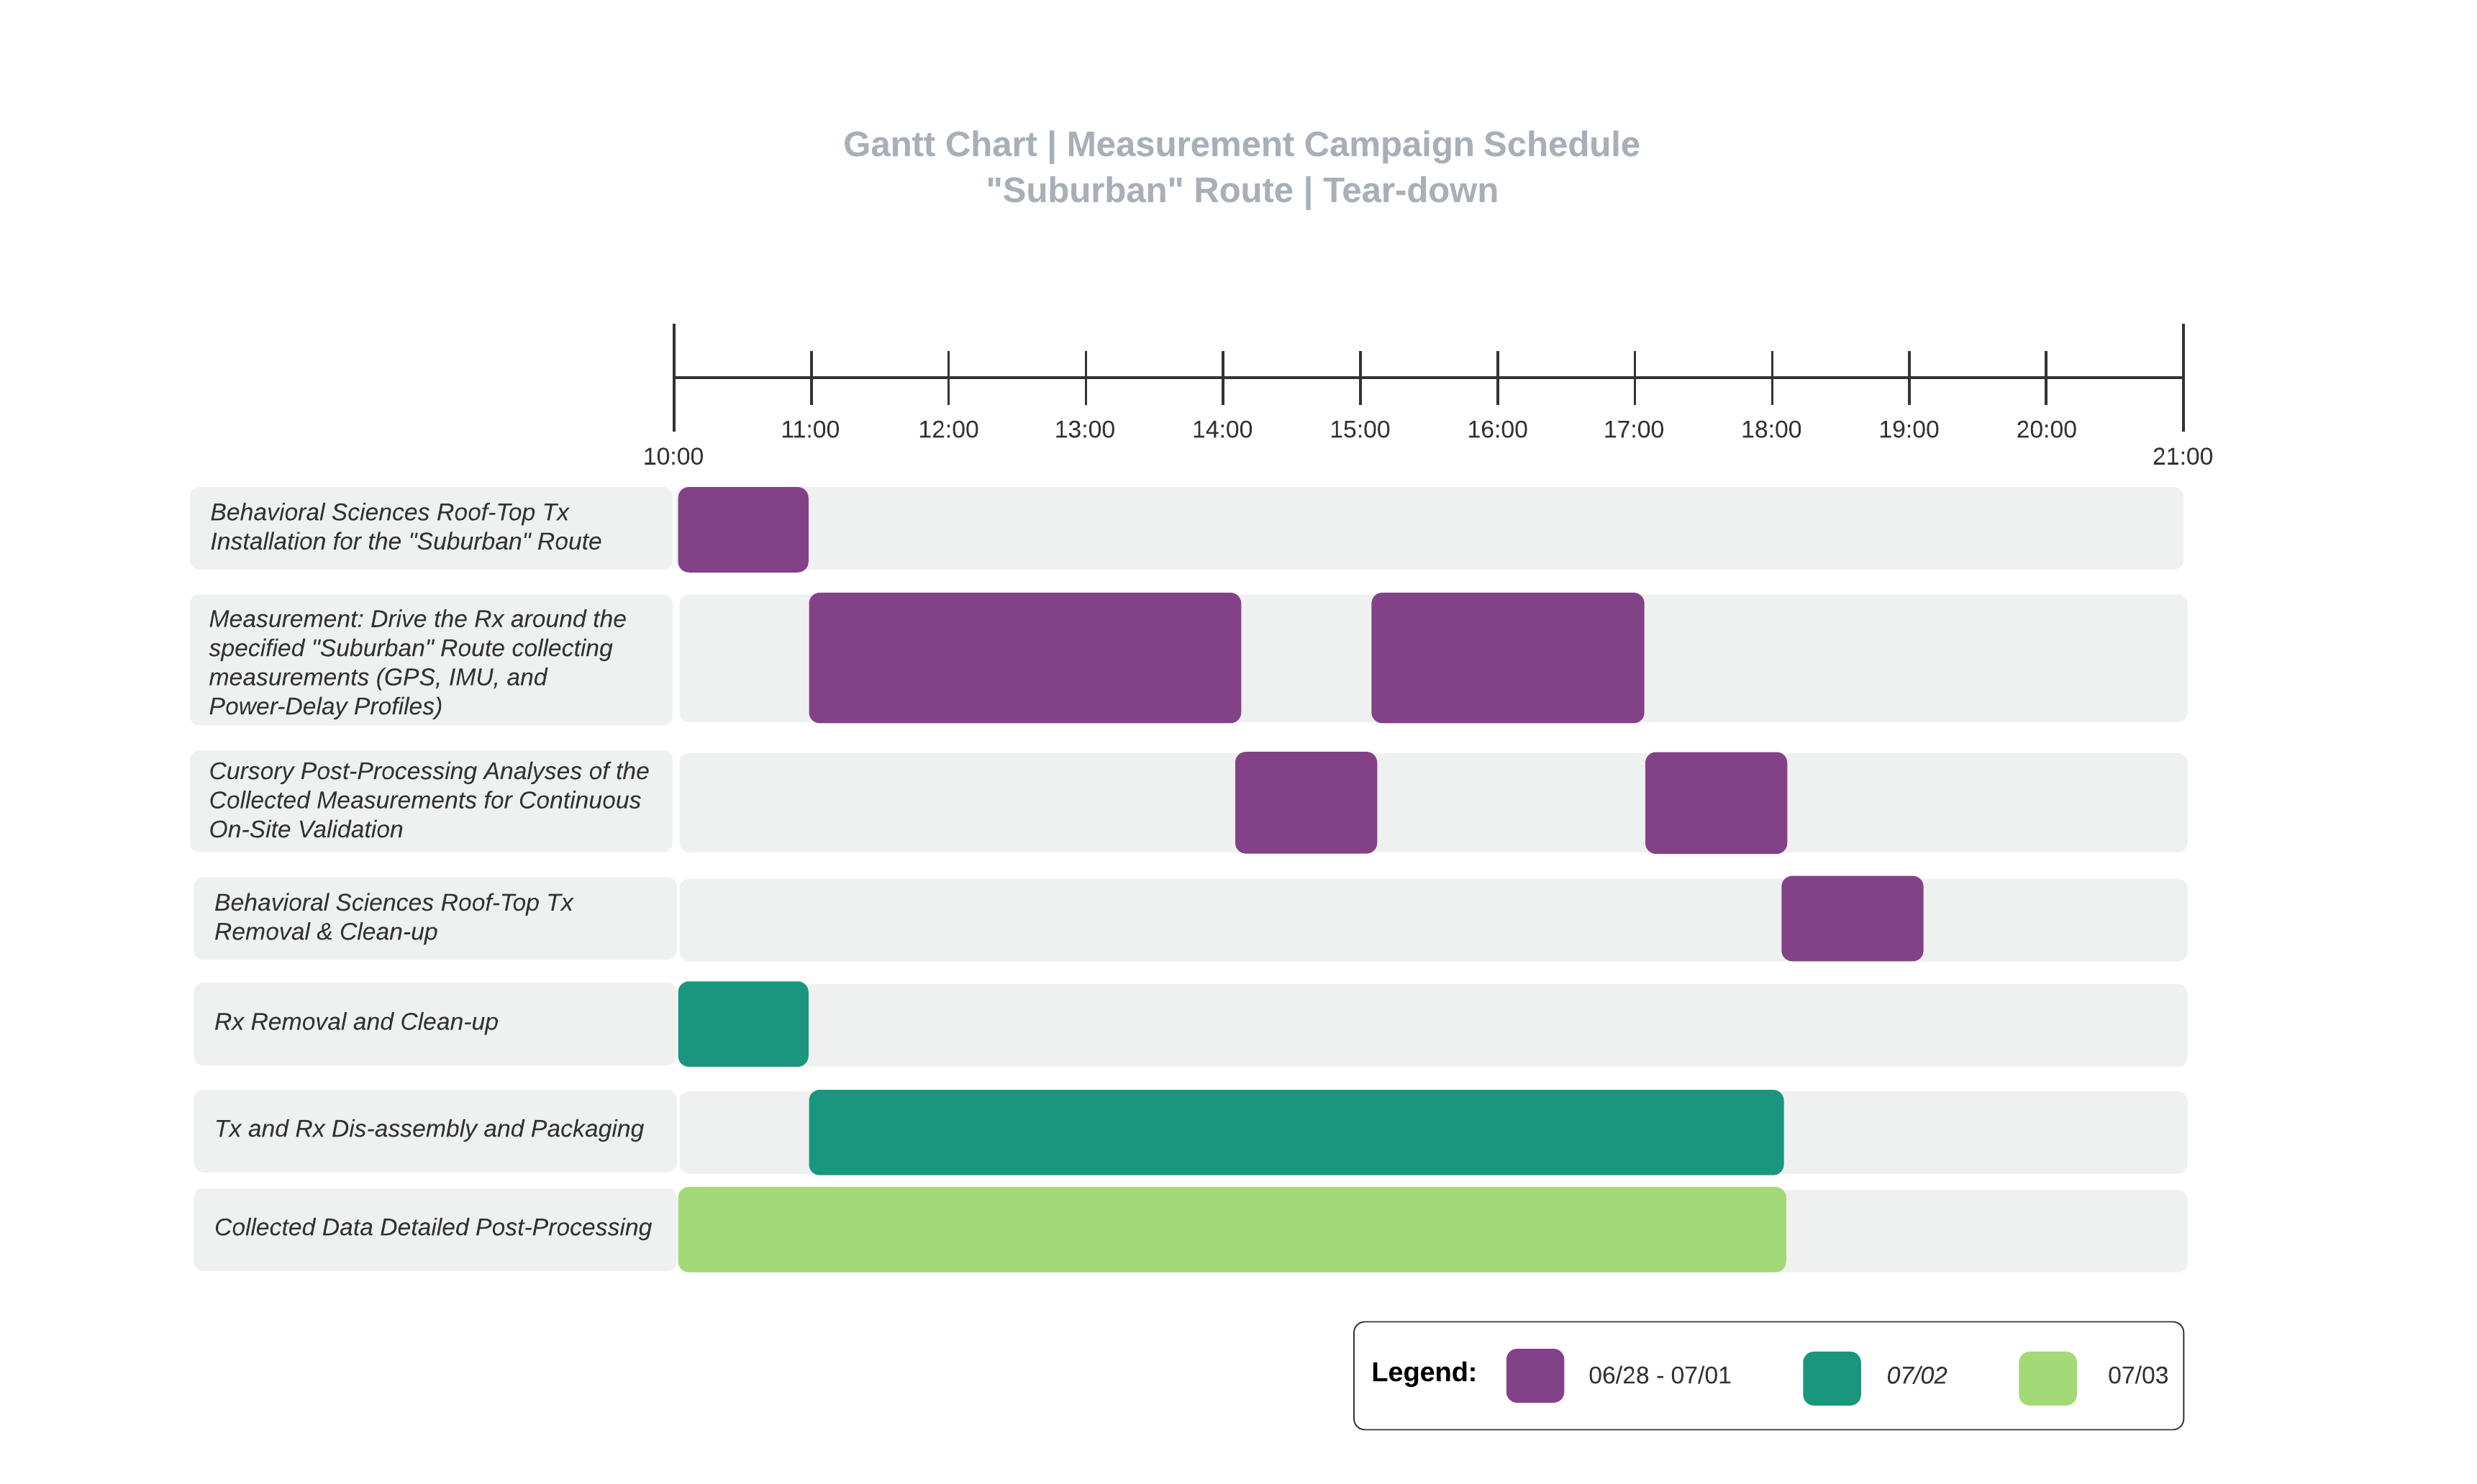
\includegraphics[width=\areaofinterestfigwidth]{figs/Odin_Measurement_Schedule_Suburban.png}
        \caption{A Gantt chart detailing our plans for data collection along the ``Suburban" route -- in addition to our timelines for system tear-down}
        \label{fig:gantt-suburban}
    \end{figure}
    \begin{figure}
        \centering
        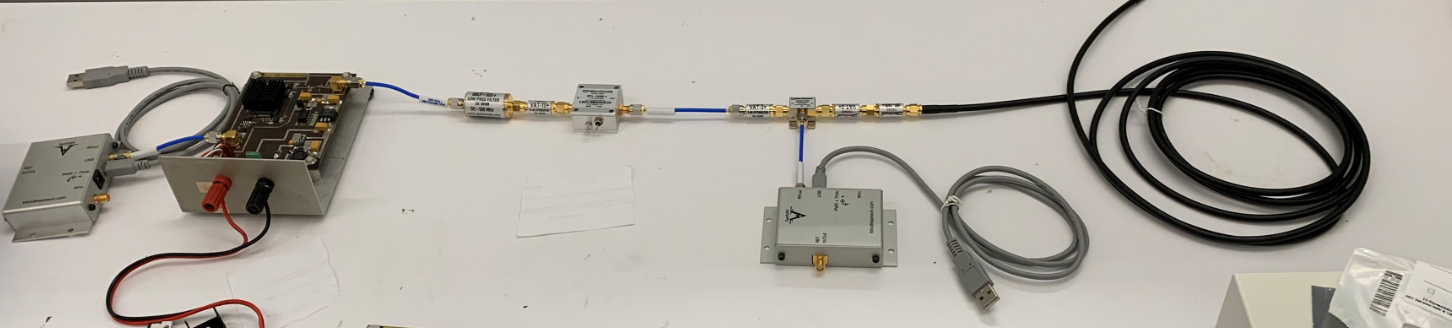
\includegraphics[width=\areaofinterestfigwidth]{figs/Tx_MiniCircuits.png}
        \caption{The Tx communication circuit components that would be encased in an ABS enclosure for weather-proofing}
        \label{fig:Tx-mini}
    \end{figure}
    \begin{figure}
        \centering
        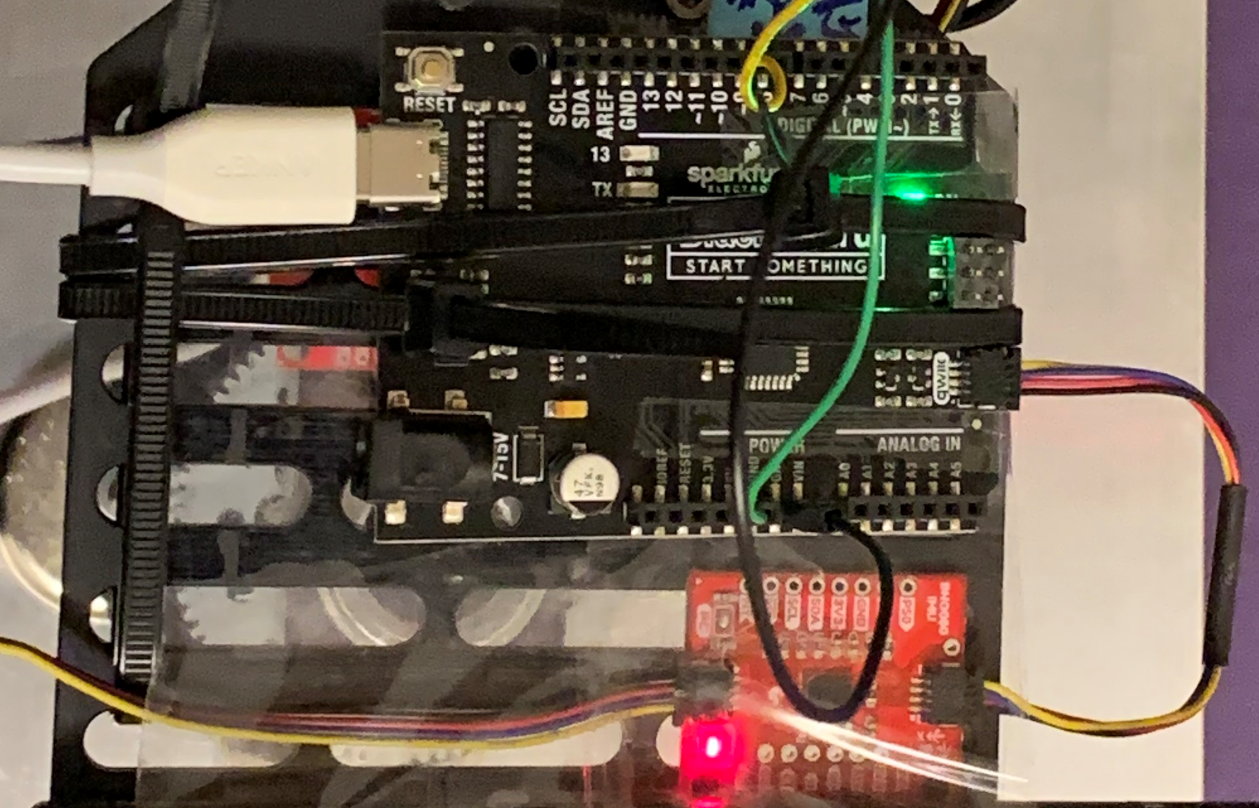
\includegraphics[width=\areaofinterestfigwidth]{figs/Prototype_Integrated_Design_3.jpg}
        \caption{The ICs (uC + IMU) corresponding to our Tx-side antenna rotating platform that would be encased in an ABS enclosure for weather-proofing}
        \label{fig:Tx-ICs}
    \end{figure}
    \begin{figure}
        \centering
        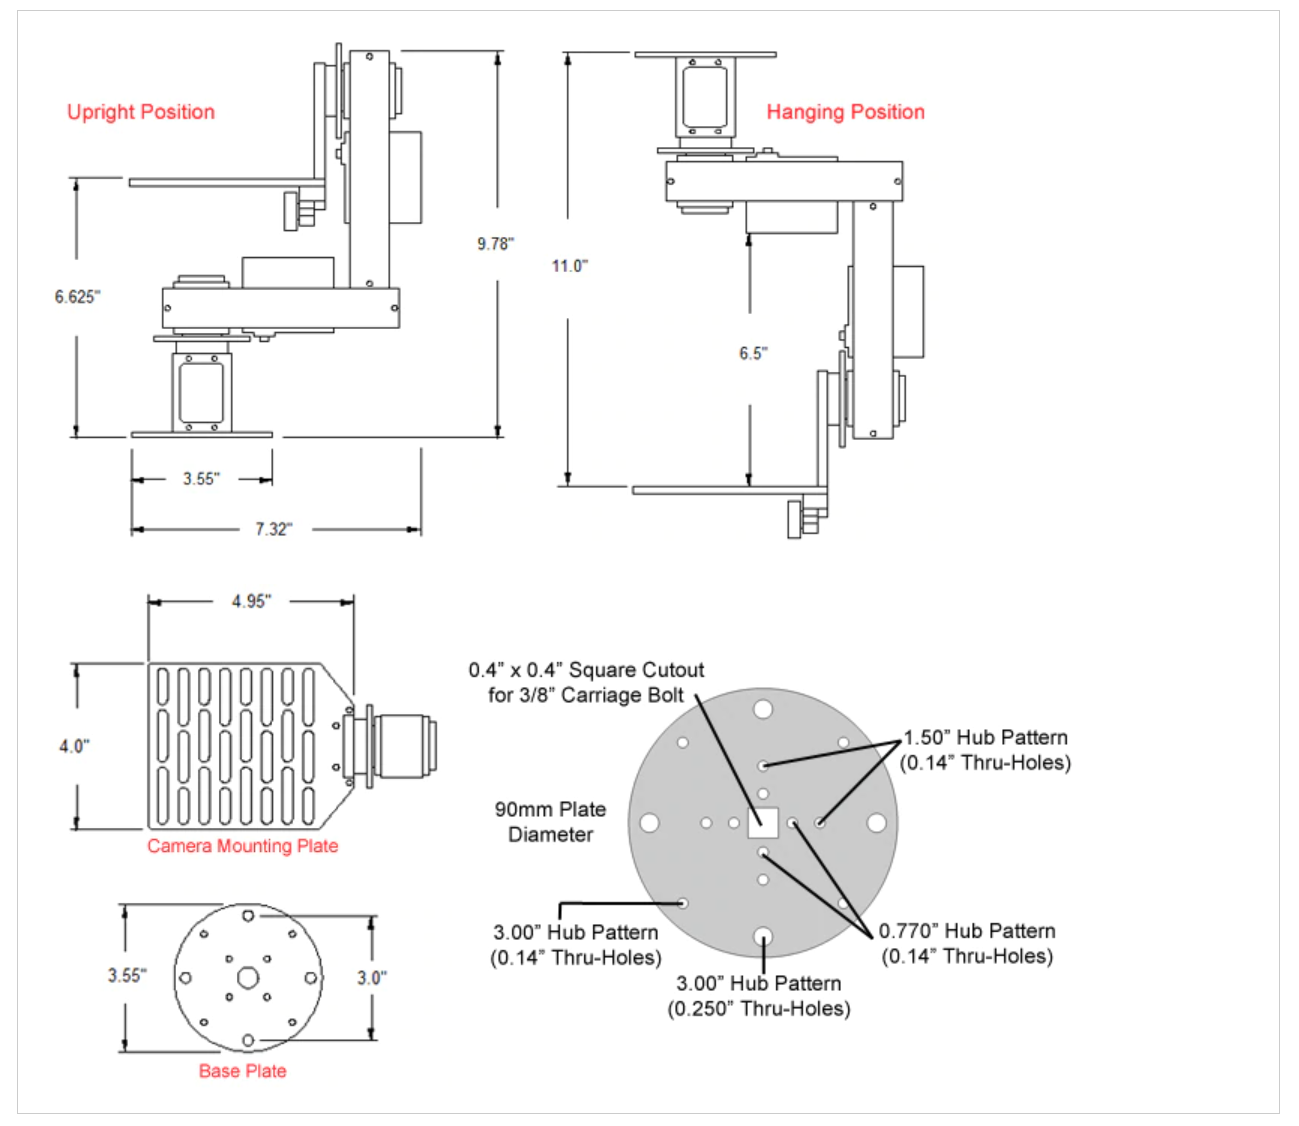
\includegraphics[width=\areaofinterestfigwidth]{figs/PT785-S_Schematics.png}
        \caption{The schematics of our Tx-side antenna rotating platform that would hold the $28$GHz WR-28 horn antenna and up-converter setup -- with servo control achieved via ICs encased in an off-platform weather-proof ABS enclosure; the Tx communication circuit components would also be housed in an off-platform weather-proof ABS enclosure}
        \label{fig:schematics}
    \end{figure}
    \subsection{Planned Measurement Campaign Schedule}
        Gantt charts detailing our measurement campaign's schedule are shown in Fig. \ref{fig:gantt-urban} and Fig. \ref{fig:gantt-suburban}: 
        \begin{itemize}
            \item Fig. \ref{fig:gantt-urban} illustrates our on-site timeline for system integration, installation, and calibration -- along with our plans for data collection while traversing the ``Blue Detour" route - with the Tx mounted on the roof-top of the University of Utah Hospital Building (ACC); and
            \item Fig. \ref{fig:gantt-suburban} illustrates our plans for data collection while traversing the ``Suburban" route - with the Tx mounted on the roof-top of the Behavioral Sciences Building -- along with our on-site timeline for system un-installation, dis-assembly, and packaging.
        \end{itemize}
    
    \subsection{Requirements to be fulfilled by POWDER Support}
        \begin{itemize}
            \item Near-edge computing resource(s) and/or Cloudlab/Emulab compute node(s) provisioning;
            \item Authorizations (FCC experimental license) to utilize the $27-29$GHz spectrum; and
            \item BYOD flexibility, i.e., authorizations and support to install the Tx at designated mount-points around the University of Utah campus:
            \begin{itemize}
                \item The base mount schematics for our Tx-side antenna rotating platform are shown in \Cref{fig:schematics}: the plan is to mount this platform via a $3/8$'' carriage bolt, and $1/4{-}20$ UNC \& $\#6{-}32$ UNC fasteners in $3$'' hub-patterns. If this hole-pattern is not available at an installation point, we plan to augment/modify the rotator's base mount to achieve compatibility (e.g., via \href{https://www.servocity.com/side-tapped-pattern-mount-f/}{\textcolor{blue}{side-tapped pattern mounts}}, \href{https://www.servocity.com/brackets/}{\textcolor{blue}{U-brackets}}, etc).
                \item No network back-haul links are needed at the Tx mount-points; instead, a laptop would be used to log the Tx-side IMU measurements. We would like to have these measurements periodically written-through to a fault-tolerant storage mechanism on a provisioned compute node: so, a good WiFi connection is preferred (not absolutely necessary).
                \item Since the Tx employs an antenna rotating platform, our system does not mandate directionality constraints during installation -- although, the Tx-side antenna rotating platform would need to be appropriately mounted to facilitate $360^\text{o}$ of rotation.
                \item Facilitate access to power for our \href{https://www.keysight.com/us/en/assets/7018-06785/data-sheets/5968-9726.pdf}{\textcolor{blue}{programmable DC power-supplies}} (x$2$): one of these is employed to output $12$V/$0.64$A for the $28$GHz antenna and up-converter system, while the other $12$V/$0.4$A for the PN-sequence generator and the ZFL-$1000$ amplifier.
                \item Facilitate weather protection at the chosen Tx sites (Sec. \ref{S3.4}):
                \begin{enumerate}
                    \item Our Tx communication circuit components (\Cref{fig:Tx-mini}) and the ICs corresponding to our Tx-side antenna rotating platform (\Cref{fig:Tx-ICs}) would be encased in separate weather-proof ABS enclosures -- along with the required weather-proof protections for any cables/wires coming-out/going-into these enclosures.\label{item1}
                    \item Our $28$GHz antenna and up-converter setup does not currently have a weather-proof dome encasing it. If this setup is to be mounted at a location where appropriate weather protections cannot be provided, we plan to design the required enclosure to weather-proof this setup.
                    \item The \href{https://www.servocity.com/pt2645-s-pan-tilt/}{\textcolor{blue}{PT2645-S Pan \& Tilt kit}}, i.e., the base antenna rotator platform, does not need weather-proofing -- however, the servo wires on this platform are weather-proofed as a part of \Cref{item1}.
                    \item The regulated power-supplies for our $28$GHz antenna and up-converter setup, ZFL-$1000$ amplifier, and PN-sequence generator would need to be placed in suitable locations at the installation point such that they are protected from adverse weather conditions.
                \end{enumerate}
            \end{itemize}
        \end{itemize}
    
\section{Sliding Correlator Channel Sounder Design}\label{S3.5}
    Our $28$GHz sliding correlator channel sounder is the same one used by us in the past for our USNA suburban measurement campaign \cite{8422820}, now integrated with our autonomous antenna tracking system (Sec. \ref{S3.6}). \Cref{fig:blocks} illustrates the overall system structure for the sounder at both the Tx and the Rx. The corresponding specifications are listed in \Cref{tab:specs}. \newline
    
    \noindent For all measurements, the pseudo-random noise (PN) rate will be set to ${\approx}400$MHz and the PN code will be an $11$-bit (length${=}2047$) sequence. The transmitter and receiver both utilize a vertically polarized horn antenna with $10^\text{o}$ half power beam-width.
    \newcommand{\tableArrayStretch}{1.41}
    \begin{table} [tb]
    	\renewcommand{\arraystretch}{\tableArrayStretch}
    	\centering
    	\begin{tabular}{| >{\bfseries}c || c |}
    		\hline
    		Carrier Frequency & $28$GHz\\
    		\hline
    		Chip Sequence Length & $2047$ \\
    		\hline
    		RF Bandwidth & $800$MHz\\
    		\hline
    		Tx Chip Rate & $400$Mcps \\
    		\hline
    		Temporal Resolution & $2.5$ns \\
    		\hline
    		Rx Chip Rate & $399.95$Mcps \\
    		\hline
    		Tx Power & $23$dBm \\
    		\hline
    		Tx/Rx Antenna Gain & $22$dBi \\
    		\hline
    		Measured Tx/Rx Azimuth HPBW & $10.1^\text{o}$ \\
    		\hline
    		Measured Tx/Rx Elevation HPBW & $11.5^\text{o}$ \\
    		\hline
    		Maximum Measurable Path Loss & $182$dB \\
    		\hline
    	\end{tabular}
    	\caption{Broadband Sliding Correlator Channel Sounder Specifications}
    	\label{tab:specs}
    \end{table}
    \clearpage
    
    \newcommand{\photosTxRxWidthRatio}{0.95}
    \begin{sidewaysfigure}[ht]
        	\centering
        	\subfloat[Transmitter]{
        		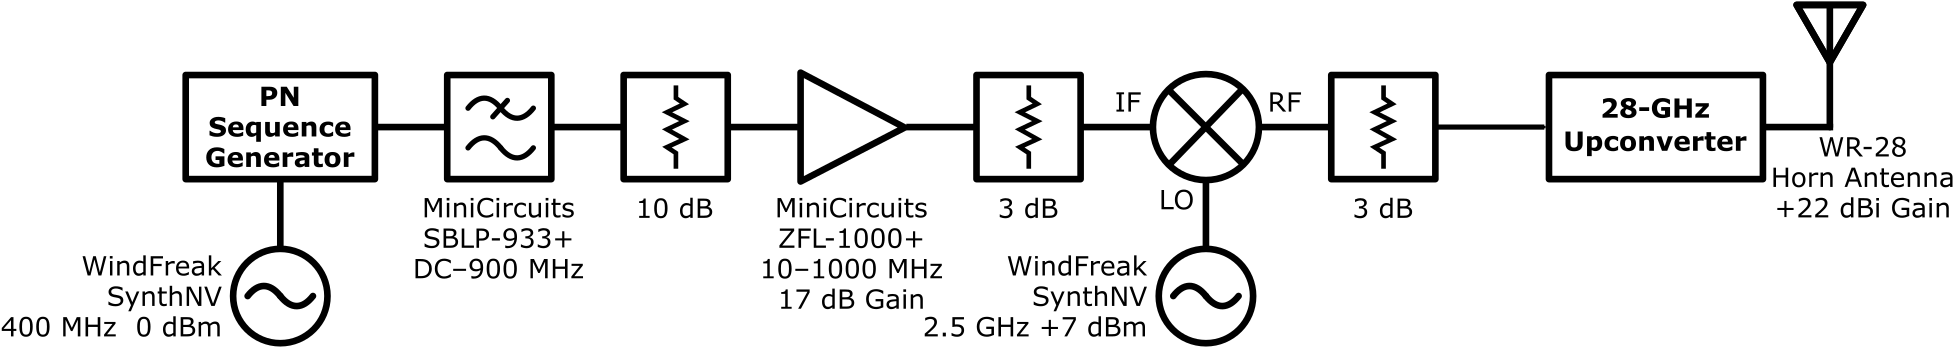
\includegraphics[width=\photosTxRxWidthRatio\textwidth]{figs/Tx.png}
        		\label{fig:block_tx}
        	}
        	\hfil
        	\subfloat[Receiver]{
        		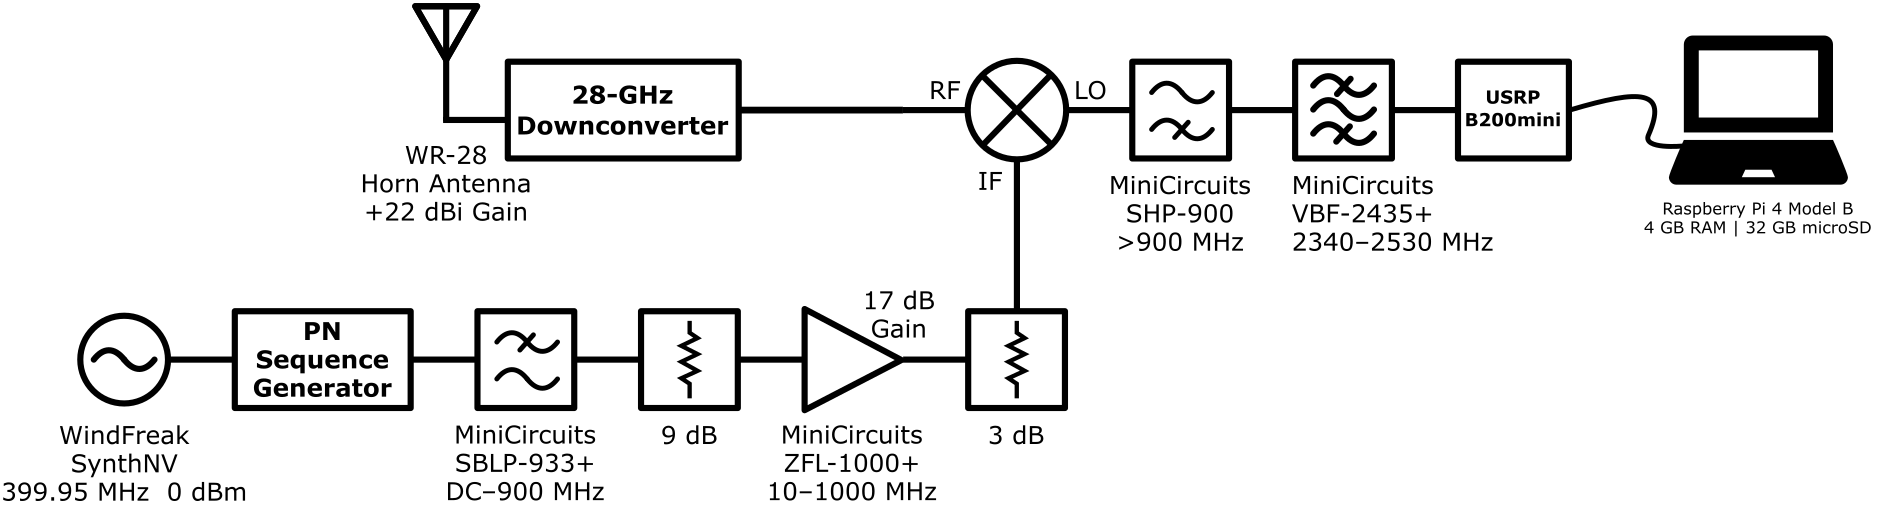
\includegraphics[width=\photosTxRxWidthRatio\textwidth]{figs/Rx_2.png}
        		\label{fig:block_rx}
        	}
        	\caption{Block diagrams for the $28$GHz broadband sliding correlator channel sounder (the model numbers are provided for some commercially available parts).}
        	\label{fig:blocks}
    \end{sidewaysfigure}
    \clearpage
    
\section{Autonomous Antenna Tracker Design}\label{S3.6}
    \begin{figure}
        \centering
        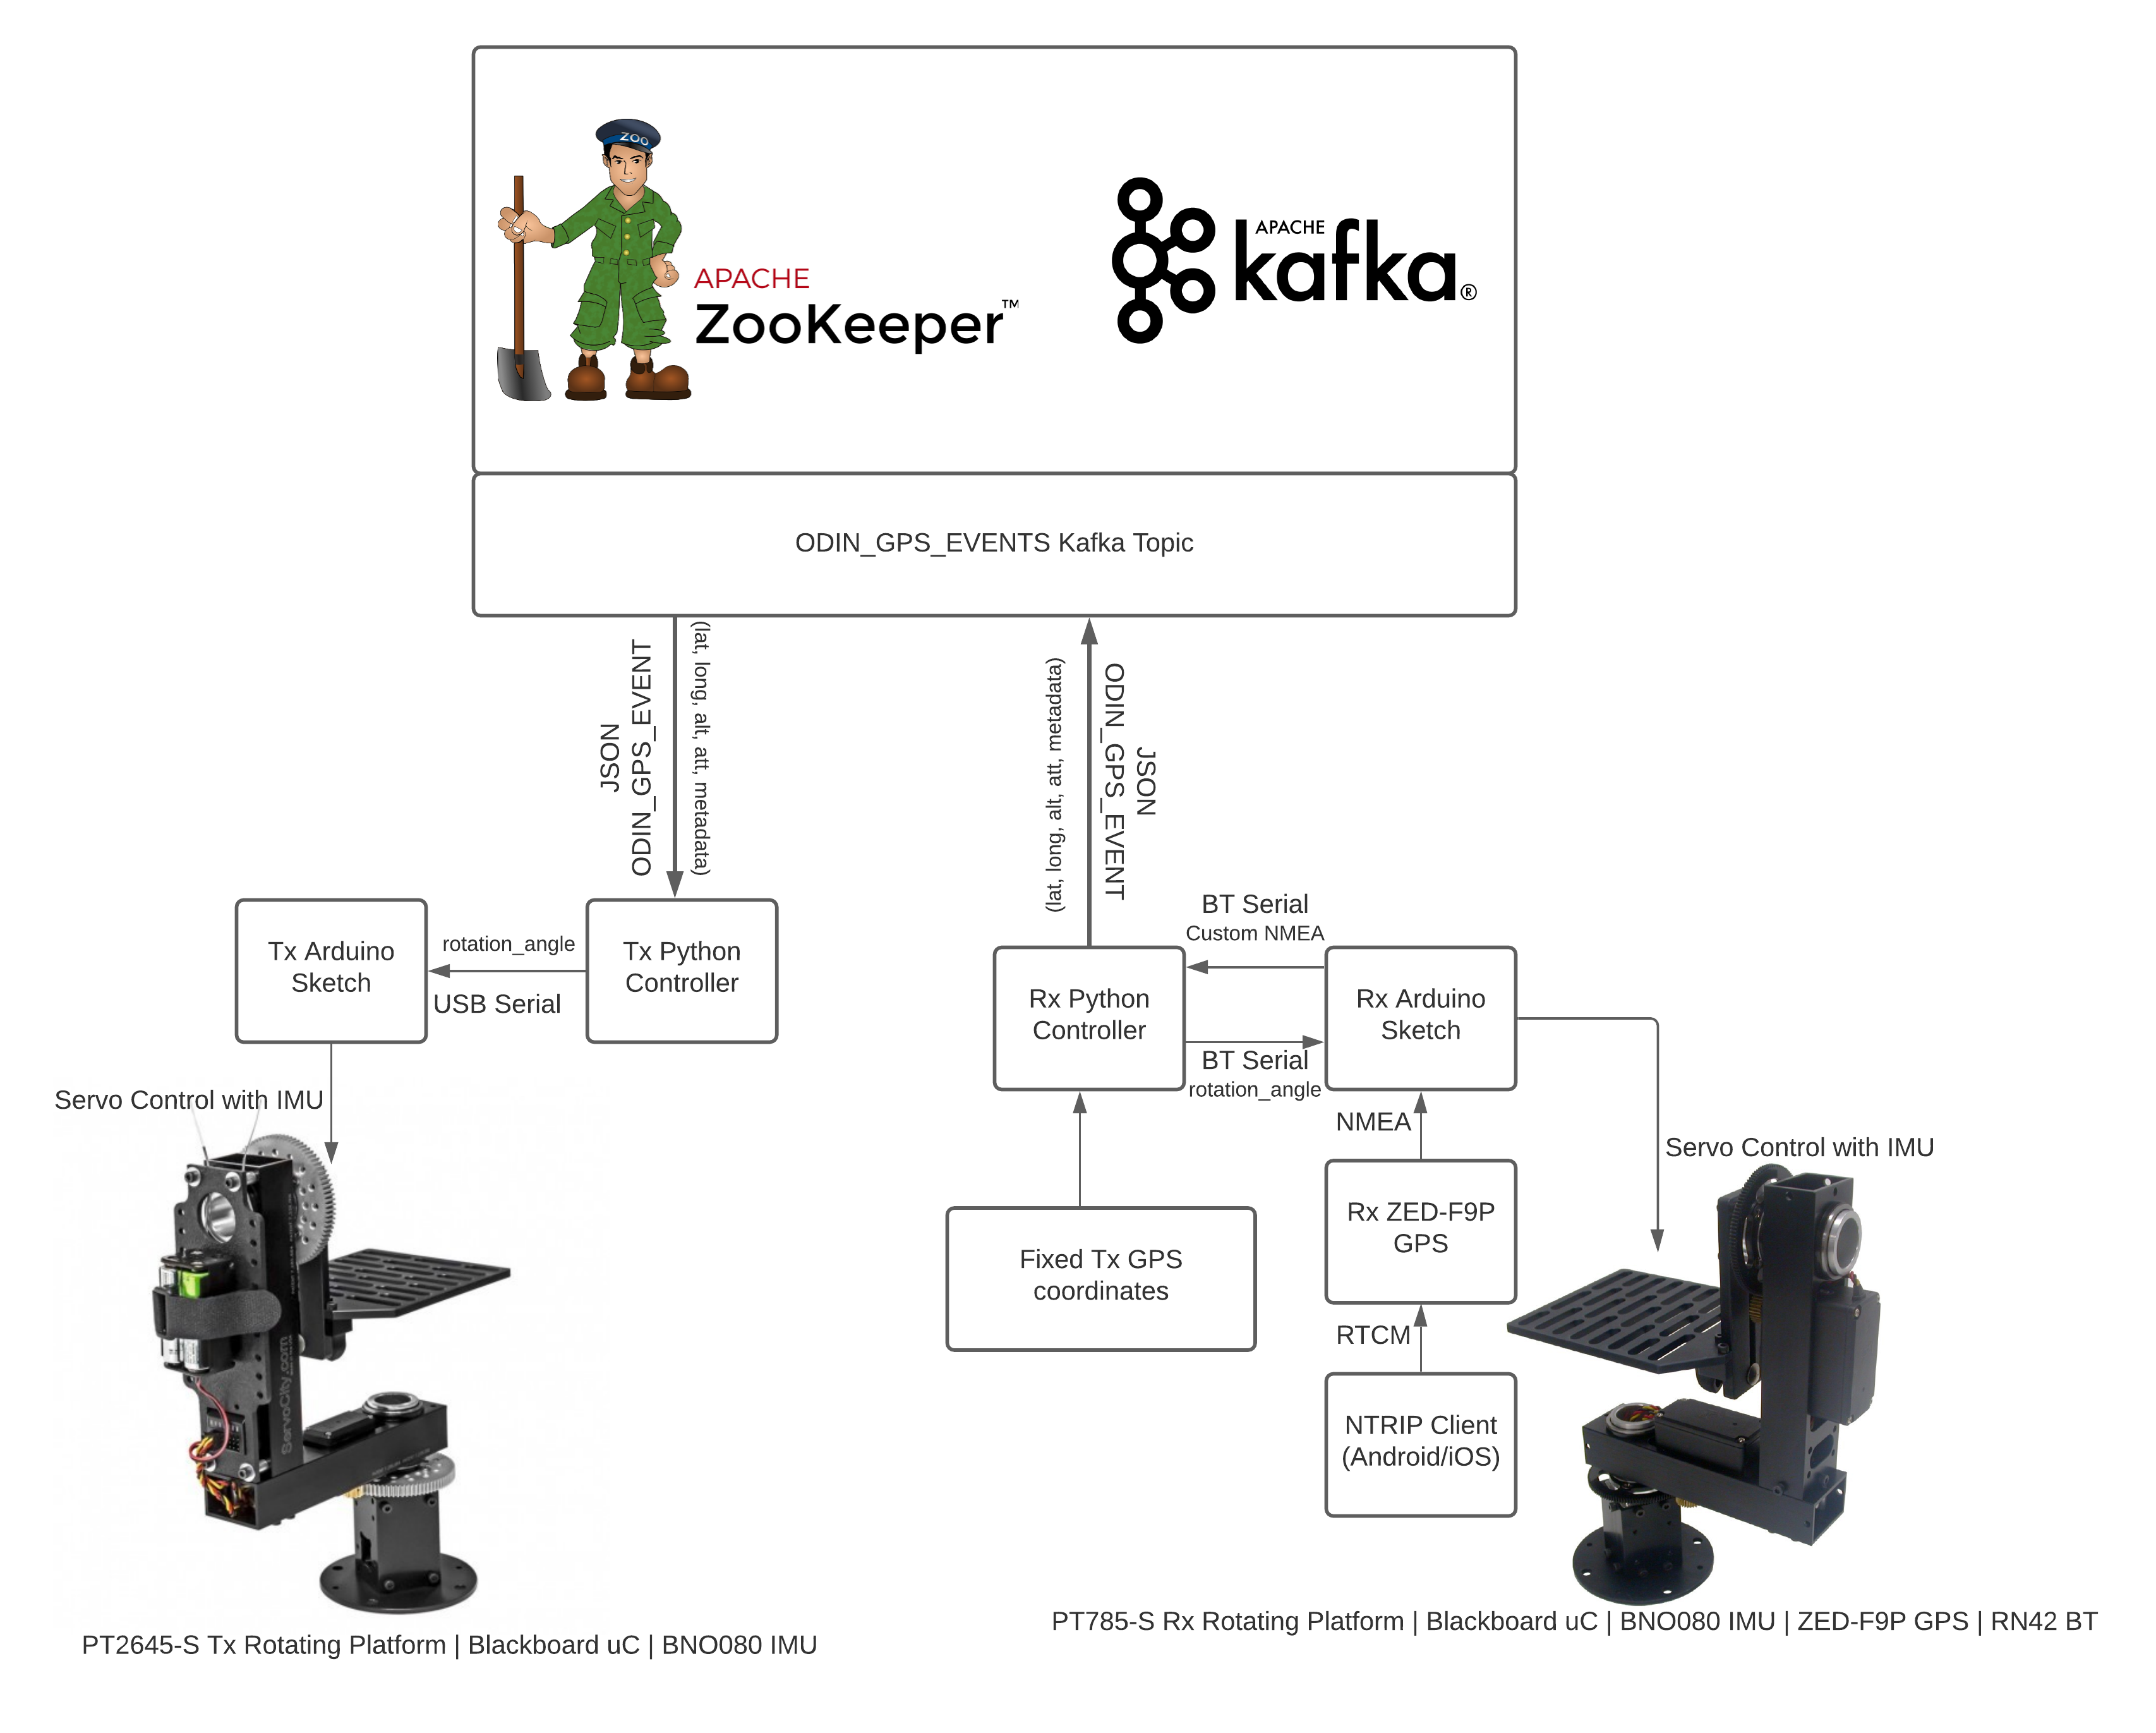
\includegraphics[width=\areaofinterestfigwidth]{figs/Odin_E2E_Design_Architecture.png}
        \caption{The E2E system architecture for the autonomous antenna rotating platforms for a mobile Rx and a fixed roof-top mounted Tx}
        \label{fig:arch}
    \end{figure}
    To ensure the antenna alignment between a fixed Tx and a mobile Rx (along both the ``pitch" and ``yaw" axes), we have implemented an autonomous antenna rotator system\footnote{Some demonstration screenshots and videos for the system can be found on \href{https://www.icloud.com/iclouddrive/0wfVsZTUo2RYsgWSQ9IMFRSYA\#Demo_Videos}{\textcolor{blue}{iCloud}}.} involving micro-controllers, IMUs, RTK-GPS modules, pan \& tilt kits, USRP B200mini SDRs, and Raspberry Pi micro-computers -- the system architecture for which is illustrated in \Cref{fig:arch}, and the associated software is encapsulated in a GitHub repository, Odin~\cite{odin}. More details about our autonomous antenna tracking system under Project Odin can be furnished upon request.

\section{Component Checklist}
\label{sec_checklist}
{
	\tabcolsep=0.083cm
	\renewcommand{\tableArrayStretch}{1.3}
	\begin{table} [h!]
	    \scriptsize
		\renewcommand{\arraystretch}{\tableArrayStretch}
		\centering
		\begin{tabu}{ | >{\bfseries}c || *{3} {c |} }
			\hline
			Component & \textbf{Reqd+Backup} & \textbf{Availability} & \textbf{Notes}\\
			\hhline{|====|}
			
			\multicolumn{4}{| c |}{\textbf{Channel Sounder - TX and RX. See \Cref{fig:blocks}.}}\\
			\hline
			WindFreak SynthNV & 3+1 & Purchased & Backups from Prof. Anderson\\
			\hline
			PN Sequence Generator & 2+1 & Custom-built & Backups from Prof. Anderson\\
			\hline
			MiniCircuits SBLP-933+ & 2+4 & Purchased & LPF | \textcolor{magenta}{4/6 Shipped}\\
			\hline
			MiniCircuits VAT-3+ & 3 & Purchased & 3dB attenuator | \textcolor{magenta}{2/3 Shipped}\\
		    \hline
			MiniCircuits K2-VAT+ & 2 & Purchased & \makecell{1dB to 10dB attenuators \\
			\textcolor{magenta}{2/2 Shipped}}\\
			\hline
			MiniCircuits ZFL-1000+ & 2+4 & Purchased & Amplifier | \textcolor{magenta}{4/6 Shipped}\\
			\hline
			MiniCircuits ZX05-43+ & 2+4 & Purchased & Mixer | \textcolor{magenta}{4/6 Shipped}\\
			\hline
			MiniCircuits SHP-900 & 1+2 & Purchased & HPF | \textcolor{magenta}{2/3 Shipped}\\
			\hline
			MiniCircuits VBF-2435+ & 1+5 & Purchased & BPF | \textcolor{magenta}{5/6 Shipped}\\
			\hline
			MiniCircuits KHFC-1+ & 1+1 & Purchased & Short coaxial cable kit\\
			\hline
			\makecell{WR-28 Horn Antenna \\with Up-converter} & 1+1 & Lent by USNA & Backup from Prof. Anderson\\
			\hline
			\makecell{WR-28 Horn Antenna \\with Down-converter} & 1+1 & Lent by USNA & Backup from Prof. Anderson\\
			\hline
			USRP B200mini & 1+1$^{*}$ & Lent by Andrew & Backup$^{*}$: USRP N310\\
			\hline
			Raspberry Pi 4 & 1+1 & Purchased & 4GB | \textcolor{magenta}{1/2 Shipped}\\
			\hline
			32GB Micro SD & 1+1 & Purchased & \makecell{For Raspberry Pi; Setup Needed; \\64GB \& 128GB cards available}\\
			\hline
			12V Power at Tx & N/A & \textcolor{blue}{Provided by POWDER} & 12V power rails at mount sites\\
			\hline
			\makecell{High-Capacity Rechargeable \\Battery at Rx} & 1+2 & Purchased & \makecell{Zeus 12V 1.3Ah | \textcolor{magenta}{2/3 Shipped}; \\Charger (x2)}\\
			\hline
			TI TPS55165Q1-EVM & 1+1 & Purchased & \makecell{Buck-Boost converter at the Rx \\\textcolor{magenta}{1/2 Shipped}}\\
			\hline
			Alligator Connectors & 13+7 & Purchased & System-wide connectivity\\
			\hline
			Intel NUC SFF & 1 & Purchased & Tx Python controller\\
            \hline
			\makecell{RG58C SMA Coaxial Cable \\10ft} & 1+3 & Purchased & \makecell{Male to 90 Degree Male \\\textcolor{magenta}{2/4 Shipped}}\\
			\hline
			\makecell{RG58C SMA Coaxial Cable \\5ft} & 1+1 & Purchased & Male to 90 Degree Male\\
			\hline
			\makecell{Low-Loss SMA Coaxial Cable \\5m-10m} & TBD & \textcolor{blue}{Provided by POWDER} & \makecell{Climate-controlled enclosure \\to pole-mounted Tx}\\
			\hline
			\makecell{SMA Female to \\N Male Adapter} & 1+1 & Purchased & \makecell{For spectrum analyzer connection; \\Tx installation \\
			\textcolor{magenta}{1/2 Shipped}}\\
			\hline
			Laptop & 1 & Personal (BK) & \makecell{Rx Python controller; \\Overall management}\\
			\hline
			External SSD & 2 & Personal (YZ) & \makecell{1TB; Secondary data storage}\\
			\hline
		\end{tabu}
	\end{table}
	
	\newpage
	\thispagestyle{empty}
    \tabcolsep=0.083cm
	\renewcommand{\tableArrayStretch}{1.3}
	\begin{table} [h!]
	    \scriptsize
		\renewcommand{\arraystretch}{\tableArrayStretch}
		\label{tab_key_para_for_chan_models}
		\centering
		\begin{tabu}{ | >{\bfseries}c || *{3} {c |} }
			\hline
			Component & \textbf{Reqd+Backup} & \textbf{Availability} & \textbf{Notes}\\
			\hhline{|====|}
			\multicolumn{4}{| c |}{\textbf{Antenna Rotating Platforms}}\\
			\hline
			ServoCity PT785-S & 0+1 & Purchased & \makecell{Closed-loop pan \& tilt kit; \\Backup for PT2645-S \\\textcolor{magenta}{1/1 Shipped}}\\
			\hline
			ServoCity PT2645-S & 2+0 & Purchased & \makecell{Open-loop pan \& tilt kit; \\
			Use PT785-S as backup}\\
			\hline
			SparkFun Blackboard C & 2+2 & Purchased & Micro-controller\\
			\hline
			\makecell{SparkFun GPS-RTK-SMA \\ZED-F9P} & 1+2 & Purchased & RTK-GPS breakout\\
			\hline
			\makecell{GPS/GNSS Magnetic-Mount \\Antenna - 3m (SMA)} & 1+2 & Purchased & \makecell{Antenna for ZED-F9P \\satellite view | \textcolor{magenta}{2/4 Shipped}}\\
			\hline
			SparkFun Bluetooth Mate Silver & 1+2 & Purchased & \makecell{Rx serial; \\RTK GPS correction data}\\
			\hline
			Portable Charger Power Bank & 4+1 & Purchased & \makecell{Component power supplies \\\textcolor{magenta}{1/5 Shipped}}\\
			\hline
			Lefebure Windows Client & 1+1 & Personal (BK+YZ) & For RTK GPS correction data\\
			\hline
			iPhone & 1 & Personal (BK) & \makecell{Wireless Hot-spot for \\Rx connectivity}\\
			\hline
			\makecell{SparkFun VR IMU\\Breakout - BNO080} & 2+2 & Purchased & Inertial Motion Unit\\
			\hline
		    SparkFun KIT-15081 & 1 & Purchased & \makecell{3 Qwiic cables; \\More needed}\\
			\hline
		    Digikey 377-2093-ND & 65+65 & Purchased & Jumpers (assorted)\\
			\hhline{|====|}
			\multicolumn{4}{| c |}{\textbf{Mounts}}\\
			\hline
			L-Bracket & 1 & Custom-built & From Prof. Anderson\\
			\hline
			\makecell{U-bolt clamp \\(3" inner diameter; \\\textgreater 4" length)} & 1+1 & Lent by USNA & From Prof. Anderson\\
			\hline
			\makecell{U-bolt clamp \\(3.5" inner diameter; \\\textgreater 4" length)} & 1+1 & Lent by USNA & From Prof. Anderson\\
			\hline
			\makecell{Metal Racks} & 1+1 & Lent by Prof. Anderson & \makecell{Tx communication circuit mount \\\textcolor{magenta}{1/2 Shipped}}\\
			\hhline{|====|}
			\multicolumn{4}{| c |}{\textbf{Tools}}\\
			\hline
			FieldFox Handheld Analyzer & 1 & Lent by Ryan & Portable Spectrum Analyzer\\
			\hline
			Magnetic Antenna Mount Set & 1+1 & Purchased & Rx installation\\
			\hline
			Tape & 1+2 & Purchased & Tx and Rx mount setup\\
			\hline
			Handheld Multi-meter & 1+1 & \textcolor{blue}{Provided by POWDER} & \makecell{Debugging the communication \\circuit components}\\
			\hline
			Keyboard + Mouse + Monitor & 1 & \textcolor{blue}{Provided by POWDER} & \makecell{USRP-GNURadio debugging}\\
			\hline
			Signal Generator & 2 & \textcolor{blue}{Provided by POWDER} & \makecell{Comm system debugging}\\
			\hline
			Spectrum Analyzer & 1 & \textcolor{blue}{Provided by POWDER} & \makecell{Comm system debugging}\\
			\hline
			Lab space & 1 & \textcolor{blue}{Provided by POWDER} & \makecell{Setup; Calibration; Debugging}\\
			\hline
			d740/d840 Compute Node & 1+2 & \textcolor{blue}{Provided by POWDER} & \makecell{Zookeeper; Kafka; \\Storage (1TB per node)}\\
			\hhline{|====|}
			\multicolumn{4}{| c |}{\textbf{Miscellaneous}}\\
			\hline
			Adjustable Attenuator & 1 & Lent by USNA & From Prof. Anderson\\
			\hline
			\makecell{ACC and Behavioral \\Rooftop Access} & N/A & \textcolor{blue}{Provided by POWDER} & \makecell{Rooftop access to \\install/uninstall Tx}\\
			\hline
			\makecell{Safety equipment} & 1+1 & \textcolor{blue}{Provided by POWDER} & Safety vests and harnesses\\
			\hline
			Go-Pros & 3 & Purchased & Vlogging\\
			\hline
		\end{tabu}
		\caption{Component checklist (Updated 6/11/2021)}
	\end{table}
	\clearpage
}

\nocite{}
\bibliographystyle{IEEEtran}
\bibliography{IEEEabrv,bibTex}

\end{document}